\documentclass{article}
%Usepackages
\usepackage{adjustbox, amsmath, amssymb, amsthm, blindtext, bm, bbm, dblfloatfix, esint, fancyhdr, float, graphicx, letltxmacro, marginnote, mathtools, subcaption, xcolor, titlesec, esint}
\usepackage{amssymb}
\usepackage[font={small, it}]{caption}
\usepackage{amsmath}
\usepackage{floatrow}
\usepackage{times}
\usepackage{ stmaryrd }
\usepackage{amsthm}
\usepackage{xcolor}
\usepackage{mathrsfs}
\usepackage[colorlinks = true,
            linkcolor = black,
            urlcolor  = blue,
            citecolor = black,
            anchorcolor = blue]{hyperref}
% \usepackage[mathscr]{euscript}
\usepackage{mathrsfs}
\usepackage{wasysym}
%\usepackage{pxfonts}
\usepackage[letterpaper, portrait, margin=1in]{geometry}
\usepackage{graphicx}
\usepackage{tikz}
\usepackage{tikz-3dplot}
\usepackage{pgfplots}
\usetikzlibrary{decorations.pathmorphing,patterns}
\usepackage{lipsum}
\usepackage{float}
\usepackage{subcaption}
\usepackage[object=vectorian]{pgfornament}
\usepackage{mwe}
\usepackage{bigints}
\usepackage{csquotes}
\usepackage{titlesec}
\usepackage{halloweenmath}
\setcounter{secnumdepth}{4}
\titleformat{\paragraph}
{\normalfont\normalsize\bfseries}{\theparagraph}{1em}{}
\titlespacing*{\paragraph}
{0pt}{3.25ex plus 1ex minus .2ex}{1.5ex plus .2ex}
\usepackage{mathtools}
\usepackage{pgfplots}
\pgfplotsset{compat=1.15}
\usepackage{lastpage}
\usepackage{enumitem}
\usepackage{tensor}
\usepackage{mathtools}

% This is for the header:
% https://tex.stackexchange.com/questions/75168/get-current-section-name-without-label
\usepackage{nameref}
\makeatletter
\newcommand*{\currentname}{\@currentlabelname}
\makeatother

\usepackage{fancyhdr} 
    \pagestyle{fancy}
    \fancyhf{}
    \fancyhead[R]{ Page \thepage \  of \pageref{LastPage}}
    \fancyhead[L]{\currentname}
\usepackage{setspace}
\usepackage{tikz}
\usetikzlibrary{hobby}

\usepackage{pst-node}
\usepackage{tikz-cd}
\usepackage[most]{tcolorbox}

% \makeatletter
% \renewcommand\@endtheorem{\vvv@endmarker\endtrivlist\@endpefalse}
% \newcommand\vvv@endmarker{%
%   {\unskip\nobreak\hfil\penalty50
%   \hskip2em\vadjust{}\nobreak\hfil\openbox
%   \parfillskip=0pt \finalhyphendemerits=0 \par
%   \penalty 10000 \parskip=0pt\noindent}\ignorespaces}
% \makeatother

\theoremstyle{definition}

% https://tex.stackexchange.com/questions/616586/how-to-make-a-tcolorbox-with-only-a-left-side-rule


\newtheorem{thm}{Theorem}[section]
\newtheorem{defn}[thm]{Definition}
\newtheorem{exmp}[thm]{Example}
\newtheorem{lem}[thm]{Lemma}
\newtheorem{conjecture}[thm]{Conjecture}
\newtheorem{exercise}[thm]{Exercise}
\newtheorem{fact}[thm]{Fact}
\newtheorem{claim}[thm]{Claim}
\newtheorem{cor}[thm]{Corollary}
\newtheorem{summary}[thm]{Summary}

\newtheorem{idea}[thm]{Idea}
\newtheorem{application}[thm]{Application}
\newtheorem{rmk}[thm]{Remark}

\newtheorem{prop}[thm]{Proposition}
\newtheorem{ques}[thm]{Question}

\newtcolorbox{cbox}[1][]{
            breakable,
            boxrule=0pt,
            frame hidden,
            sharp corners,
            enhanced,
            borderline west={2pt}{0pt}{#1},
            colback=#1!5!white}

% \newenvironment{cthm}[3]
%     {\begin{cbox}[#2]
%     \color{#2}
%     \begin{#3}[#1]
%     \color{black}
%     }
%     {
%     \end{#3} 
%     \end{cbox}
%     }

% \newenvironment{theorem}[1][]
% {\begin{cthm}{#1}{orange}{thm}}
% {\end{cthm}}

\newenvironment{theorem}[1][]
    {\begin{cbox}[blue]
    \color{blue}
    \begin{thm}[#1]
    \color{black}
    }
    {
    \end{thm} 
    \end{cbox}
    }

\newenvironment{corollary}[1][]
    {\begin{cbox}[orange]
    \color{orange}
    \begin{cor}[#1]
    \color{black}
    }
    {
    \end{cor} 
    \end{cbox}
    }

\newenvironment{lemma}[1][]
    {\begin{cbox}[orange]
    \color{orange}
    \begin{lem}[#1]
    \color{black}
    }
    {
    \end{lem} 
    \end{cbox}
    }

\newenvironment{proposition}[1][]
    {\begin{cbox}[orange]
    \color{orange}
    \begin{prop}[#1]
    \color{black}
    }
    {
    \end{prop} 
    \end{cbox}
    }

\newenvironment{definition}[1][]
    {\begin{cbox}[red]
    \color{red}
    \begin{defn}[#1]
    \color{black}
    }
    {
    \end{defn} 
    \end{cbox}
    }

\newenvironment{example}[1][]
    {\begin{cbox}[violet]
    \color{violet}
    \begin{exmp}[#1] \color{black}
    }
    {
    \end{exmp} 
    \end{cbox}
    }

\newenvironment{question}[1][]
    {\begin{cbox}[black]
    \begin{ques}[#1]
    }
    {
    \end{ques} 
    \end{cbox}
    }

\newenvironment{remark}[1][]
    {\begin{cbox}[black]
    \begin{rmk}[#1]
    }
    {
    \end{rmk} 
    \end{cbox}
    }



\newenvironment{solution}
  {\renewcommand\qedsymbol{$\blacksquare$}\begin{proof}[Solution]}
  {\end{proof}}
\newenvironment{answer}
  {\begin{proof}[Answer]}
  {\end{proof}}
  
% \newenvironment{example}
%   {\pushQED{\qed}\renewcommand{\qedsymbol}{$\triangle$}\examplex}
%   {\popQED\endexamplex}


%%%%%%%%%%%%%%%%%%%%%%%%%%%%%

%Custom Commands
    \renewcommand\qedsymbol{$\blacksquare$}
    \newcommand{\Pcal}{\mathcal{P}}
    \newcommand{\ve}{\varepsilon}
    \newcommand{\Ocal}{\mathcal{O}}
    \newcommand{\Asf}{\textsf{A}}
    \newcommand{\al}{\alpha}
    \newcommand{\be}{\beta}
    \newcommand{\Nbb}{\mathbb{N}}
    \newcommand{\Si}{\Sigma}
    \newcommand{\Hbb}{\mathbb{H}}
    \DeclareMathOperator{\diag}{diag}
    \newcommand{\De}{\Delta}
    \newcommand{\Xcal}{\mathcal{X}}
    \newcommand{\si}{\sigma}
    \newcommand{\Ga}{\Gamma}
    \newcommand{\Cscr}{\mathscr{C}}
    \newcommand{\1}{\mathbf{1}}
    \newcommand{\Dcal}{\mathcal{D}}
    \newcommand{\Iscr}{\mathscr{I}}
    \newcommand{\Pbb}{\mathbb{P}}
    \newcommand{\B}{\mathbb{B}}
    \newcommand{\Dscr}{\mathscr{D}}
    \newcommand{\Nfrak}{\mathfrak{N}}
    \newcommand{\Efrak}{\mathfrak{E}}
    \DeclareMathOperator{\charp}{charpoly}
    \newcommand{\Csf}{\mathsf{C}}
    \newcommand{\rfrak}{\mathfrak{r}}
    \newcommand{\Sbb}{\mathbb{S}}
    \newcommand{\La}{\Lambda}
    \newcommand{\de}{\delta}
    \DeclareMathOperator{\inte}{int}
    \DeclareMathOperator{\ord}{ord}
    \newcommand{\set}{\mathsf{set}}
    \newcommand{\Bscr}{\mathscr{B}}
    \newcommand{\Zscr}{\mathscr{Z}}
    \newcommand{\ab}{\mathrm{ab}}
    \newcommand{\Xscr}{\mathscr{X}}
    \newcommand{\Escr}{\mathscr{E}}
    \newcommand{\Gscr}{\mathscr{G}}
    \DeclareMathOperator{\Sym}{Sym}
    \newcommand{\om}{\omega}
    \newcommand{\gfrak}{\mathfrak{g}}
    \newcommand{\hfrak}{\mathfrak{h}}
    \newcommand{\kfrak}{\mathfrak{k}}
    \newcommand{\Grp}{\mathsf{Grp}}
    \newcommand{\Ab}{\mathsf{Ab}}
    \newcommand{\xbar}{\bar{x}}
    \newcommand{\abar}{\bar{a}}
    \newcommand{\ybar}{\bar{y}}
    \DeclareMathOperator{\coker}{coker}
    \newcommand{\Modsf}{\mathsf{Mod}}
    \newcommand{\op}{\mathrm{op}}
    \newcommand{\Ring}{\mathsf{Ring}}
    \newcommand{\modsf}{\mathsf{mod}}
    \DeclareMathOperator{\Alt}{Alt}
    \newcommand{\Om}{\Omega}
    \newcommand{\ze}{\zeta}
    \newcommand{\Fcal}{\mathcal{F}}
    \newcommand{\Oscr}{\mathscr{O}}
    \newcommand{\gl}{\mathfrak{gl}}
    \DeclareMathOperator{\Lie}{Lie}
    \DeclareMathOperator{\GL}{GL}
    \DeclareMathOperator{\SL}{SL}
    \DeclareMathOperator{\Vol}{Vol}
    \DeclareMathOperator{\Disc}{Disc}
    \DeclareMathOperator{\SO}{SO}
    \newcommand{\Xfrak}{\mathfrak{X}}
    \DeclareMathOperator{\id}{id}
    \DeclareMathOperator{\Int}{Int}
    \DeclareMathOperator{\End}{End}
    \DeclareMathOperator{\Aut}{Aut}
    \DeclareMathOperator{\stab}{stab}
    \DeclareMathOperator{\orb}{orb}
    \DeclareMathOperator{\grad}{grad}
    \DeclareMathOperator{\curl}{curl}
    \newcommand{\vp}{\varphi}
    \newcommand{\vt}{\vartheta}
    \DeclareMathOperator{\Gal}{Gal}
    \DeclareMathOperator{\rank}{rank}
    \DeclareMathOperator{\col}{col}
    \DeclareMathOperator{\Tame}{Tame}  
    \newcommand{\Yscr}{\mathscr{Y}}
    \newcommand{\Fbb}{\mathbb{F}}
    \newcommand{\Hcal}{\mathcal{H}}
    \newcommand{\arctanh}{\text{arctanh}}
    \newcommand{\pa}{\partial}
    \newcommand{\del}{\boldsymbol{\nabla}}
    \newcommand{\na}{\nabla}
    \newcommand{\Ycal}{\mathcal{Y}}
    \DeclareMathOperator{\spn}{span}
    \DeclareMathOperator{\Inn}{Inn}
    \DeclareMathOperator{\chara}{char}
    \newcommand{\lap}{\nabla^2}
    \newcommand{\Pfrak}{\mathfrak{P}}
    \newcommand{\mfrak}{\mathfrak{m}}
    \newcommand{\Fvec}{\mathbf{F}}
    \newcommand{\Mcal}{\mathcal{M}}
    \newcommand{\ellvec}{\boldsymbol{\ell}}
    \newcommand{\rvec}{\mathbf{r}}
    \DeclareMathOperator{\supp}{supp}
    \newcommand{\Abb}{\mathbb{A}}
    \newcommand{\svec}{\mathbf{s}}
    \newcommand{\VECT}{\mathsf{VECT}}
    \newcommand{\fs}{\vec{\sigma}}
    \newcommand{\bs}{\cev{\sigma}}
    \newcommand{\uvec}{\mathbf{u}}
    \newcommand{\iunit}{\boldsymbol{\hat{\i}}}
    \newcommand{\junit}{\boldsymbol{\hat{\j}}}
    \newcommand{\xunit}{\mathbf{\hat{x}}}
    \newcommand{\Char}{\text{char}}
    \newcommand{\kunit}{\mathbf{\hat{k}}}
    \newcommand{\theunit}{\boldsymbol{\hat{\theta}}}
    \newcommand{\pvec}{\mathbf{p}}
    \newcommand{\qvec}{\mathbf{q}}
    \newcommand{\Qcal}{\mathcal{Q}}
    \newcommand{\yvec}{\mathbf{y}}
    \newcommand{\xvec}{\mathbf{x}}
    \newcommand{\wvec}{\mathbf{w}}
    \newcommand{\bvec}{\mathbf{b}}
    \newcommand{\Ucal}{\mathcal{U}}
    \newcommand{\Ncal}{\mathcal{N}}
    \newcommand{\Scal}{\mathcal{S}}
    \newcommand{\Nscr}{\mathscr{N}}
    \newcommand{\da}{\dagger}
    \newcommand{\CT}{\mathrm{H}}
    \newcommand{\Sscr}{\mathscr{S}}
    \DeclareMathOperator{\lcm}{lcm}
    \newcommand{\evec}{\mathbf{e}}
    \newcommand{\Kscr}{\mathscr{K}}
    \newcommand{\ebold}{\boldsymbol{e}}
    \newcommand{\zvec}{\mathbf{z}}
    \newcommand{\vvec}{\mathbf{v}}
    \newcommand{\Tscr}{\mathscr{T}}
    \newcommand{\avec}{\mathbf{a}}
    \newcommand{\Avec}{\mathbf{A}}
    \newcommand{\Ivec}{\mathbf{I}}
    \newcommand{\ivec}{\mathbf{i}}
    \newcommand{\jvec}{\mathbf{j}}
    \newcommand{\kvec}{\mathbf{k}}
    \newcommand{\of}{\mathfrak{o}}
    \DeclareMathOperator{\Ot}{O}
    \DeclareMathOperator{\Sy}{S}
    \newcommand{\slf}{\mathfrak{sl}}
    \newcommand{\muvec}{\boldsymbol{\mu}}
    \newcommand{\Bvec}{\mathbf{B}}
    \newcommand{\Cvec}{\mathbf{C}}
    \newcommand{\eunit}{\mathbf{\hat{e}}}
    \newcommand{\vpunit}{\boldsymbol{\hat{\varphi}}}
    \newcommand{\zero}{\boldsymbol{0}}
    \newcommand{\tauvec}{\boldsymbol{\tau}}
    \newcommand{\runit}{\mathbf{\hat{r}}}
    \newcommand{\U}{\mathcal{U}}
    \newcommand{\Zbb}{\mathbb{Z}}
    \newcommand{\Bsf}{\mathsf{B}}
    \DeclareMathOperator{\G}{G}
    \newcommand{\gmat}{\textsf{g}}
    \newcommand{\Ccal}{\mathcal{C}}
    \newcommand{\SM}{\mathsf{SM}}
    \newcommand{\VB}{\mathsf{VB}}
    \newcommand{\Dsf}{\mathsf{D}}
    \newcommand{\Fscr}{\mathscr{F}}
    \DeclareMathOperator{\Map}{Map}
    \DeclareMathOperator{\Frob}{Frob}
    \newcommand{\Imat}{\textsf{I}}
    \newcommand{\Rmat}{\textsf{R}}
    \DeclareMathOperator{\Frac}{Frac}
    \DeclareMathOperator{\Spec}{Spec}
    \DeclareMathOperator{\Emb}{Emb}
    \newcommand{\Kcal}{\mathcal{K}}
    \newcommand{\Wcal}{\mathcal{W}}
    \newcommand{\Lcal}{\mathcal{L}}
    \newcommand{\Tcal}{\mathcal{T}}
    \newcommand{\Ecal}{\mathcal{E}}
    \DeclareMathOperator{\im}{im}
    \newcommand{\Qbb}{\mathbb{Q}}
    \newcommand{\ga}{\gamma}
    \newcommand{\la}{\lambda}
    \newcommand{\RomanNumeralCaps}[1]
        {\MakeUppercase{\romannumeral #1}} 
    \newcommand{\dif}{\text{d}}
    \newcommand{\Rbb}{\mathbb{R}}
    \newcommand{\Tbb}{\mathbb{T}}
    \DeclareMathOperator{\Hom}{Hom}
    \DeclareMathOperator{\conv}{conv}
    \newcommand{\Vcat}{\mathsf{V}}
    \newcommand{\Gr}{\text{Gr}}
    \newcommand{\Bcal}{\mathcal{B}}
    \newcommand{\Acal}{\mathcal{A}}
    \newcommand{\pfrak}{\mathfrak{p}}
    \newcommand{\qfrak}{\mathfrak{q}}
    \newcommand{\Evec}{\mathbf{E}}
    \newcommand{\omvec}{\boldsymbol{\omega}}
    \newcommand{\alvec}{\boldsymbol{\alpha}}
    \newcommand{\gvec}{\mathbf{g}}
    \newcommand{\afrak}{\mathfrak{a}}
    \newcommand{\bfrak}{\mathfrak{b}}
    \newcommand{\Cbb}{\mathbb{C}}
    \newcommand{\gavec}{\boldsymbol{\gamma}}
    \newcommand{\Tvec}{\mathbf{T}}
    \newcommand{\Vscr}{\mathscr{V}}
    \newcommand{\Ascr}{\mathscr{A}}
    \newcommand{\Uscr}{\mathscr{U}}
    \newcommand{\Sfrak}{\mathfrak{S}}
    \DeclareMathOperator{\sgn}{sgn}
    \DeclareMathOperator{\vol}{vol}
    \newcommand{\Pscr}{\mathscr{P}}
    \newcommand{\Wscr}{\mathscr{W}}
    \newcommand{\bcdot}{\boldsymbol{\cdot}}
    \DeclareMathOperator{\tr}{tr}
    
    \newcommand{\sectionline}{
        \noindent
        \begin{center}
        {
        {{
        {\begin{tikzpicture}
        \node  (C) at (0,0) {};
        \node (D) at (16,0) {};
        \path (C) to [ornament=89] (D);
        \end{tikzpicture}}}}}
        \end{center}
        }
    \newcommand{\sectionlineflip}{
        \noindent
        \begin{center}
        {
        {{
        {\begin{tikzpicture}
        \node  (C) at (0,0) {};
        \node (D) at (16,0) {};
        \path (D) to [ornament=89] (C);
        \end{tikzpicture}}}}} 
        \end{center}
        }
        

        
       
%%%%%%%%%%%%%%%%%%%%%%%%%%%%%%%
%Custom Symbols
\newcommand{\goodemptyset}[1]{%
\begin{tikzpicture}[#1]%
\draw (0,0) circle (0.1);%
\draw(-0.07,-0.14)--(0.07,0.14);
\end{tikzpicture}%
}

\newcommand{\es}{\raisebox{-1pt}{\goodemptyset{}}}


\makeatletter
\DeclareRobustCommand{\cev}[1]{%
  {\mathpalette\do@cev{#1}}%
}
\newcommand{\do@cev}[2]{%
  \vbox{\offinterlineskip
    \sbox\z@{$\m@th#1 x$}%
    \ialign{##\cr
      \hidewidth\reflectbox{$\m@th#1\vec{}\mkern4mu$}\hidewidth\cr
      \noalign{\kern-\ht\z@}
      $\m@th#1#2$\cr
    }%
  }%
}
\makeatother


\makeatletter
\DeclarePairedDelimiterX{\pmodx}[1]{(}{)}{{\operator@font mod}\mkern6mu#1}
\renewcommand{\pmod}{%
  \allowbreak
  \if@display\mkern18mu\else\mkern8mu\fi
  \pmodx
}
\makeatother
\DeclarePairedDelimiter\bra{\langle}{\rvert}
\DeclarePairedDelimiter\ket{\lvert}{\rangle}
\DeclarePairedDelimiterX\braket[2]{\langle}{\rangle}{#1 \delimsize\vert #2}

 
\makeatletter
\newcommand{\colim@}[2]{%
  \vtop{\m@th\ialign{##\cr
    \hfil$#1\operator@font colim$\hfil\cr
    \noalign{\nointerlineskip\kern1.5\ex@}#2\cr
    \noalign{\nointerlineskip\kern-\ex@}\cr}}%
}
\newcommand{\colim}{%
  \mathop{\mathpalette\colim@{\rightarrowfill@\scriptscriptstyle}}\nmlimits@
}
\renewcommand{\varinjlim}{%
  \mathop{\mathpalette\varlim@{\rightarrowfill@\scriptscriptstyle}}\nmlimits@
}
\renewcommand{\varprojlim}{%
  \mathop{\mathpalette\varlim@{\leftarrowfill@\scriptscriptstyle}}\nmlimits@
}

\newcommand{\mjedit}[1]{{\color{orange}  #1}}
\newcommand{\mattie}[1]{{\color{orange} \sf $\clubsuit\clubsuit\clubsuit$ Mattie: [#1]}}
\newcommand{\margMa}[1]{\normalsize{{\color{red}\footnote{{\color{orange}#1}}}{\marginpar[{\color{red}\hfill\tiny\thefootnote$\rightarrow$}]{{\color{red}$\leftarrow$\tiny\thefootnote}}}}}
\newcommand{\Mattie}[1]{\margMa{(Mattie) #1}}


% %%%%%%%%%%%%%%%%%%%%%%%%%%%%%
% %Just arrows (cause normy arrows suck)
% \newcommand{\goodarrow}[1]{
% \begin{tikzpicture}[#1]
% \draw[-stealth] (0,0)--(0.4,0);
% \end{tikzpicture}
% }

% \renewcommand{\to}{\raisebox{2.4pt}{\hspace{0.08cm}\goodarrow{}\hspace{0.06cm}}}

% %%%%

% \newcommand{\goodtwoheadrightarrow}[1]{
% \begin{tikzpicture}[#1]
% \draw[->>, >=stealth] (0,0)--(0.4,0);
% \end{tikzpicture}
% }

% \renewcommand{\twoheadrightarrow}{\raisebox{2.4pt}{\hspace{0.08cm}\goodtwoheadrightarrow{}\hspace{0.06cm}}}

% %%%

% \newcommand{\goodhookrightarrow}[1]{
% \begin{tikzpicture}[#1]
% \draw[right hook-stealth] (0,0)--(0.4,0);
% \end{tikzpicture}
% }

% \renewcommand{\hookrightarrow}{\raisebox{2.3pt}{\hspace{0.08cm}\goodhookrightarrow{}\hspace{0.06cm}}}

% %%%

% \newcommand{\goodmapsto}[1]{
% \begin{tikzpicture}[#1]
% \draw[-stealth] (0,0)--(0.4,0);
% \draw[] (0,0.06)--(0,-0.06);
% \end{tikzpicture}
% }

% \renewcommand{\mapsto}{\raisebox{0pt}{\hspace{0.02cm}\goodmapsto{}\hspace{0.03cm}}}


% %%%%%%%%%%%%%%%%%%%%%%%%%%%%%

% \tikzcdset{arrow style=tikz, diagrams={>={stealth[round,length=4pt,width=4.5pt,inset=2.75pt]}}}






\renewcommand*\contentsname{Table of Content}

\title{APMA 2550: Numerical Solutions (Approximation) of PDEs I}
\author{Notes taken by Mattie Ji}
\date{Updated \today}
\setlength\parindent{0pt}

\begin{document}

\maketitle
These are lecture notes from \textbf{APMA 2550: Numerical Solutions (Approximation) of PDEs I} with Professor Mark Ainsworth at Brown University for the Fall 2023 semester. The most up-to-date version of the notes are maintained under my GitHub \href{https://github.com/maroon-scorch}{repository}.\\

These notes are taken by Mattie Ji with gracious help and input from the instructor of this course. If you find any mistakes in these notes, please feel free to direct them via email to me or send a pull request on GitHub.\\

The notes are last updated \today.
\tableofcontents
\newpage

\section{Lecture 1}

\subsection{Logistics}

\begin{itemize}
    \item \textbf{When: } We meet at Barus and Holley $3:00 - 5:20$ pm every Wednesday. We will take a $10$ minute break in the middle of lecture.
    \item \textbf{Assessment: } The grade of the class is divided into 2 components: Coursework is $80\%$ and the Final Project is $20\%$.
    
    Courseworks are homeworks assigned each Wednesday and due the following Wednesday before class. They are not meant to be busy work but as complementary materials for the course that might be challenging. Professor Ainsworth strongly believes in learning by doing assignments.

    We have a final project in this course because this class is to train future researchers. The final project itself will be more of computational nature and may have some applications.
    
    \item \textbf{Syllabus and Books: }

    \begin{remark}
    This is Professor Ainsworth's first time teaching this course. He has taught Part II and III before, but this is his first time teaching Part I. This is because, apparently, this class gets a lot of feedback as being ``boring". Another source of frustation is whenever he has a time-dependnet PDE, he would like his students to know how to solve it, but apparently past iterations of Part I never taught this. 
    \end{remark}

    The focus of this course is on time-discretization methods, ie. we want to solve time dependent PDEs/ODEs. This is a very classical topic and is so successful that barely anyone does research in this field anymore, but there are some very nice methods for us to know in this class.

    There are no recommended textbooks for this course, but there are some books you may consider:
    \begin{enumerate}
        \item J. D. Lambert, \textit{Numerical Methods for Ordinary Differential Systems: The Initial Value Problem}
        \item Volumes I to III of $\{$Hairer, Noursett, Wanner, Lubich$\}$, all about 500 pages each.
        \item Lots of other books...
    \end{enumerate}

    \item \textbf{Programming Languages for this class: }
    \begin{enumerate}
        \item What the instructor personally prefers: \texttt{C++}
        \item What the students can use: \texttt{Julia}, \texttt{Python}, \texttt{Matlab} (it would be alright for the class but instructor does not recommend), \texttt{C++}, \texttt{Fortran}, \texttt{ADA}.
        \item \texttt{Maple} and \texttt{Mathematica} aren't really recommended since they are algebraic manipulation packages and is not good at memory handling.
    \end{enumerate}

    \item \textbf{Prerequisites: } 
    \begin{enumerate}
        \item Working knowledge of real analysis. We will have theoretical portions in this class.
     \begin{remark}
        The \textbf{Sleipner C Oil Platform} was an incident where an oil field blew up (it measured a $5$ on the earthquake Richter scale. What happened was the numerical analysts used a completely incorrect method to do the calculations. A lot of workers involved were sent to jail due to professional negligence. This is why we care about the ``analysis" part of numerical analysis.
    \end{remark}
        \item Some familiarity with programming.
        \item You have seen ODEs and PDEs before.
    \end{enumerate}
    But we will cover some relevant contents in these topics when needed.
\end{itemize}


\subsection{Ordinary Differential Equations}

ODEs arise naturally whenever we model any time dependent system.

\begin{example}[Cooling of a Body]
Suppose we have a cup of tea with temperature $u(t)$ at time $t$. The ambient temperature is $T$ that we assume is lower than $u(t)$. In this case, tea cools because the ambient temperature is lower than $u(t)$.
\[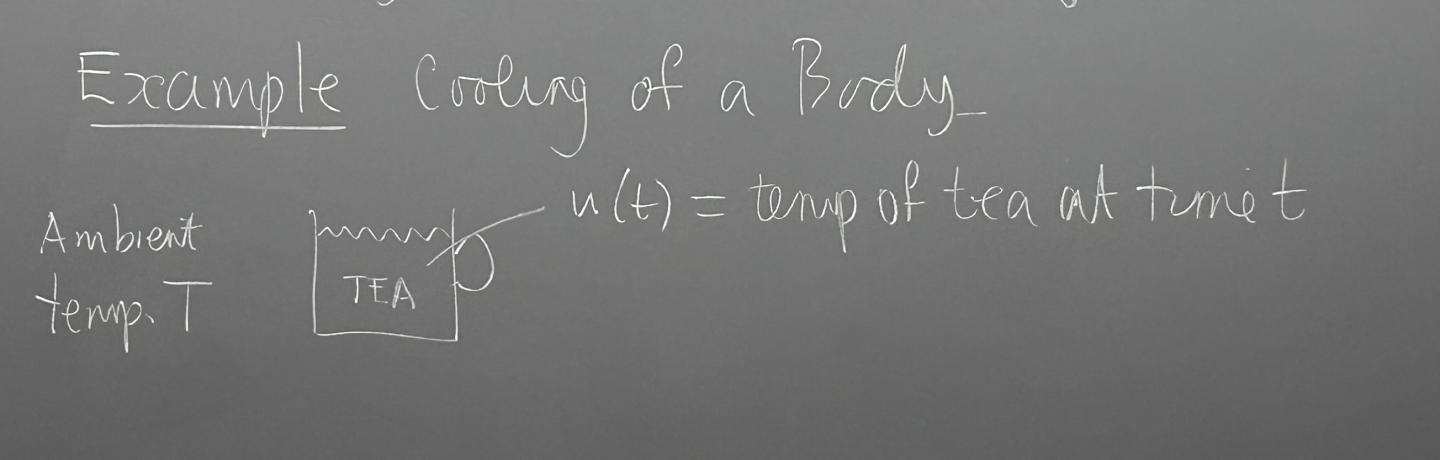
\includegraphics[width=0.6\textwidth]{Figures/lecture1/lec1-1.png}\]
Consider the system at time $t$ and time $t + \delta t$. Hear energy is conserved in this system. The heat energy in the cup at time $t$
 is
 \[m_T c_T u(t)\]
 where $m_T$ is the mass of the tea and $c_T$ is the specific heat capacity of the tea. The heat energy at time $t + \delta t$ is
 \[m_T c_T u(t + \delta t) = m_T c_T u(t) - \{\text{Heat lost to the surroundings}\}\]

\begin{question}
    How much heat is lost?
\end{question}

The amount of heat is lost should be dependent on the difference $u(t) - T$, the surface area of the cup, and should be proporitional to $\delta t$ (provided that it is really small so we can do a local linear approximation). There could also be vapor going out with some convection going out, but we will ignore it for now by Ainsworth's Principle of Maximum Laziness.\\

Hence the amount of heat lost could be modeled as
\[\alpha (u(t) - T) \delta t\]
where $\alpha > 0$ is some constant that measures the ``physical attributes" of the cup.\\

Hence, the heat energy at time $t + \delta t$ can be given as
\[m_T c_T u(t + \delta t) = m_T c_T u(t) - \alpha (u(t) - T) \delta t\]
This equation implies that
\[\frac{ u(t + \delta t) - u(t)}{\delta t} = - \beta (u(t) + T)\]
where $\beta = \frac{\alpha}{m_T c_T} > 0$. Taking the limit as $\delta t \to 0$, we have that
\[u'(t) = - \beta (u(t) - T)\]
Finally, we add an initial condition specifying that $u(t_0) = u_0$.\\

Solving the ODE using standard techniques of calculus, we obtained that
\[u(t) = T + (u_0 - T) e^{-\beta t}, t \geq 0\]

Observe that as $t \to \infty$, we have that
\[u(t) \to T\]

This question is an example of a linear, first order, initial value problem. This is called \textbf{Newton's Law of Cooling}.
 \end{example}

 \begin{example}
     What if we replace the cup of tea with the planetary phenonmenon ``black body"?
     \[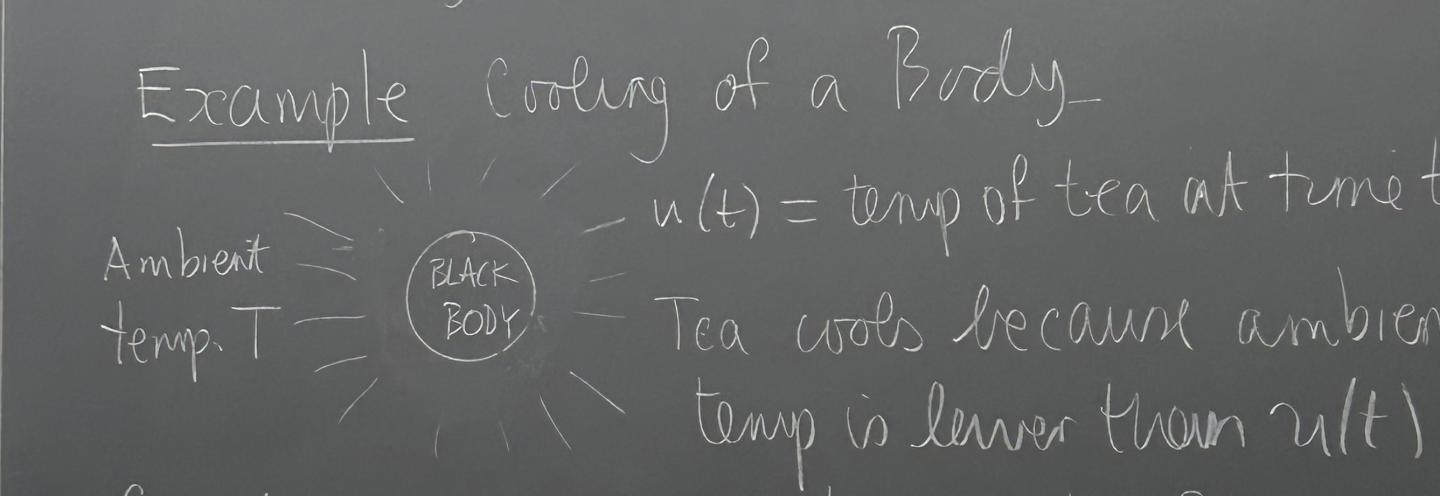
\includegraphics[width=0.6\textwidth]{Figures/lecture1/lec1-2.png}\]
     \textbf{Stefan's Law of Black Body Radiation} says that the heat energy lost should be proportional to $(u(t) - T)^4$ instead of $(u(t) - T)$ and we have
     \[\alpha_1 (u(t) - T) + \alpha_4 (u(t) - T)^4\]
     for $\alpha_1, \alpha_4 \geq 0$.\\

     This leads to an initial valued problem:
     \[u'(t) = - \beta_1 (u(t) - T) - \beta_4 (u(t) - T)^4, u(t_0) = u_0\]
     The solution of this can be done in analytic form, but it is not as easy as the previous example.
     \begin{question}
         How do we proceed from here? It depends on who you ask.
     \end{question}
     \begin{itemize}
         \item \textbf{Dynamical system approach: }In this case, we look for an equilibrium and cosnider the RHS
         \[f(u) = - \beta_1 (u - T) - \beta_4 (u - T)^4\]
         An equilibrium (critical point) is here if and only if $f(u) = 0$.
         
         For example $u = T$ is an example of a equilibrium. $\beta_1 + \beta_4 (u - T)^3 = 0$ is another solutions, which is true if and only if $u = T - (\frac{\beta_1}{\beta_4})^{1/3} < T$. These are the only two equilibriums of the system. The graph looks somewhat like:
       \[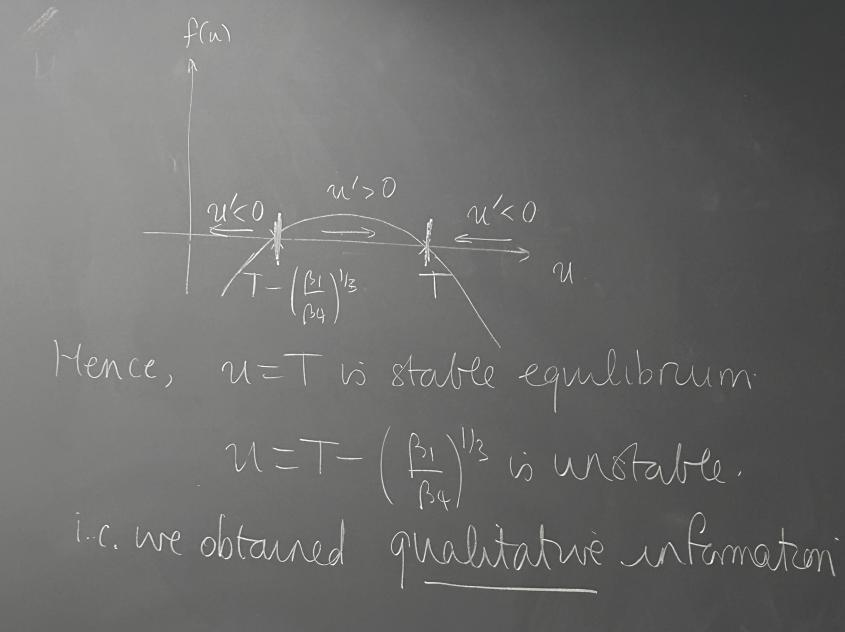
\includegraphics[width=0.6\textwidth]{Figures/lecture1/lec1-3.png}\]
        Hence, $u = T$ is a stable equilibrium and $u = T - (\frac{\beta_1}{\beta_4})^{1/3}$ is an unstable equilibrium. We have obtained \textbf{qualitative information} about the system. However, sometimes we need \textbf{quantitative information} about a system, ie. we want a sufficiently accurate approximatin of this solution.
        
        The physics is also a little dodgy for $t < T - (\frac{\beta_1}{\beta_4})^{1/3}$ since the model implies temperature would run off the negative infinity here.
        \item \textbf{Numerical PDE/ODE approach: } This is how we will get quantitative information. Even then, the type of numerics you want to do could depend on what you are trying to do. For example, if your numerical method does not perserve energy, then to physics this is unacceptable. So you might want to sacrifice accuracy to perserve energy. That's why there are a lot of studies around this topic.

        Numerical PDE/ODE isn't just asking a computer to output some answers. There's a methodology in selecting the right tools and tackling the right questions.
     \end{itemize}
 \end{example}

Let's do another example
\begin{example}[Population Growth]
    Let $N(t)$ be the population at time $t$ and we want to look at how $N(t)$ grows as $t$ changes. The simple method is to model
    \[N(t + \delta t) = N(t) + \delta t [\alpha_B N(t) -  \alpha_D N(t)]\]
    where $\alpha_B \geq 0$ indicates the birth rate and $\alpha_D \geq 0$ indicates the death rate. We have again that
    \[\frac{N(t + \delta t) - N(t)}{\delta t} = (\alpha_B - \alpha_D) N(t)\]
    When we take the limit, we have that
    \[N'(t) = (\alpha_B - \alpha_D) N(t), N(0) = N_0\]
    The behavior as $t \to \infty$ depends on the sign of $\alpha_B - \alpha_D$ as when when solve the equation, we get
    \[N(t) = N_0 e^{(\alpha_B - \alpha_D) t}\]
    Notice that
    \[\lim_{t \to \infty} N(t) = \begin{cases}
    \infty, \alpha_B > \alpha_D\\
    0, \alpha_B < \alpha_D\\
    N_0, \alpha_B = \alpha_D
    \end{cases}\]
This behavior does not make sense in real life, and our model does not account for (finite resources, diseases, etc.)\\

Let $\alpha = \alpha_B - \alpha_D$, let's instead model this as the \textbf{logistics equation}
\[N(t + \delta t) = N(t) + \delta t \alpha N(t) - \delta t \beta N(t)^2 \]
where $\beta$ accounts for resource management and we make the reasonable assumption that resource management squares as population grows. It also tries to take account of diseases, etc. Hence we have that
\[N'(t) = \alpha N(t) - \beta N(t)^2\]

This could be solved analytically, but it is somewhat complicated.

Let's pretend again that we are dynamical systems students, then let
\[f(N) = \alpha N - \beta N^2\]
Then we have that $f(N) = 0$ if and only if $N = 0$ or $N = \frac{\alpha}{\beta} > 0$, and the graph is
\[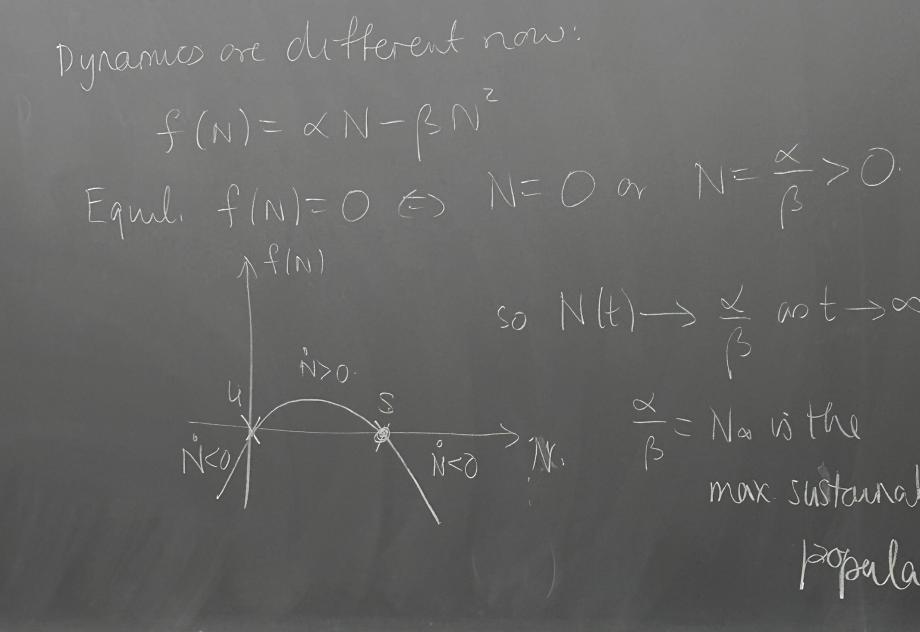
\includegraphics[width=0.6\textwidth]{Figures/lecture1/lec1-4.png}\]
Hence we expect $N(t)$ to tend towards the equilibrium at $\alpha/\beta$. We call $N_\infty = \frac{\alpha}{\beta}$ as the maximum sustainable population.\\

Let's also look at \textbf{spatial effects}, suppose we have an island $\Omega$ where the population is on the island:
\[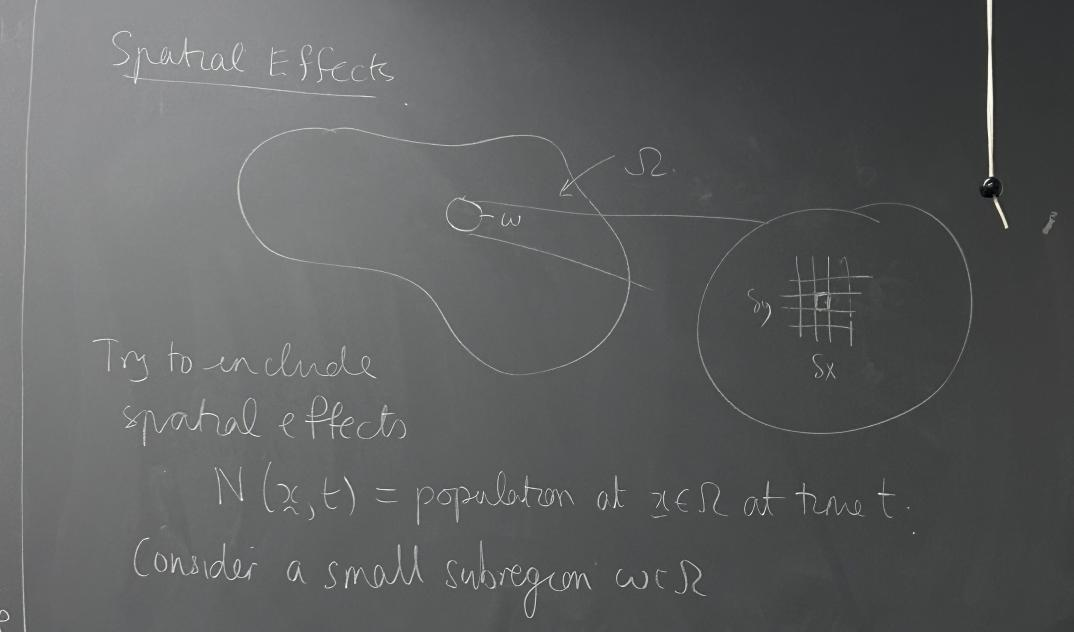
\includegraphics[width=0.6\textwidth]{Figures/lecture1/lec1-5.png}\]
We want $N(x, t)$ to be the population at $x \in \Omega$ and time $t$. Consider a small subregion $\omega \subset \Omega$, and let's let $N_w(t)$ be the population in $\omega$ at time $t$, note that
\[N_w(t) = \int_{w} N(x, t) dx\]
By the principle of conservation of people, we need to take account of the birth and death rate and the immigration rate on the boundary:
\[N_w(t + \delta t) = N_w(t) + \delta t \int_w dx \left(\alpha N(x, t) - \beta N(x, t)^2 \right) - \{\text{immigration at $\partial \omega$ during $(t, t + \delta t)$}\} \]
Let's call a small arc of the boundary as $\delta s$, we make the assumption that people go from more dense place to less dense places.\\

Let's define a flux $\sigma(x, t)$ which is proportional to the spatial gradient $-\nabla N(x, t)$ (the minus sign is here since we are going from more dense places to less dense places). So we write our \textbf{constructive equation}
\[\sigma(x, t) = - \gamma \nabla N, \gamma > 0\]

Hence, the outflow across $\delta s << 1$ should be $\delta s \sigma(x, t) \cdot n$, where $n$ is the unit outward normal vector.
\[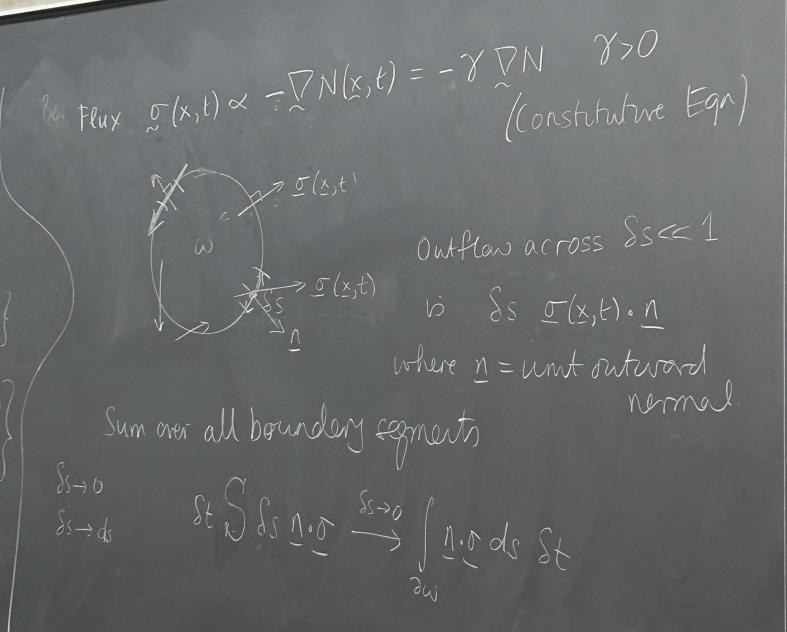
\includegraphics[width=0.6\textwidth]{Figures/lecture1/lec1-6.png}\]
When we sum over all the boundary segments, the immigration effect is 
\[\lim_{\delta s \to 0} \delta t \sum \delta s n \cdot \sigma = \delta t \int_{\partial w} n \cdot \sigma ds \]
Hence, we have that
\begin{align*}
    \int_\omega N(x, t + \delta t) dx &= \int_w N(x, t) dx + \delta t \int_w (\alpha N - \beta N^2) dx - \delta t \int_{\partial w} n \cdot \sigma ds\\
    \iff \int_w \frac{N(x, t + \delta t) - N(x, t)}{\delta t} dx &= \int_w (\alpha N - \beta N^2) dx - \int_w dw \sigma dx \tag*{Divergence Theorem}
\end{align*}
If we take the limit as $\delta t \to 0$ and substitute for $\sigma$, we have that
\[\int_w \frac{\partial N}{\partial t} dx = \int_w (\alpha N - \beta N^2 + \gamma \Delta N) dx\]
for all subregion $w \subset \Omega$. Let ``$w \to 0$" (let the region go smaller and smaller), that is we will divide both side by area of $w$ - $|w|$, and we take $|w| \to 0$:
\[\frac{1}{|w|} \int_w \frac{\partial N}{\partial t} dx = \frac{1}{|w|}  \int_w (\alpha N - \beta N^2 + \gamma \Delta N) dx\]
Assuming $N$ is smooth, taking the limit $|w| \to 0$, we will concentrate at a specific point $x \in w$, gives us
\[\frac{\partial N}{\partial t} = \alpha N - \beta N^2 + \delta \Delta N \text{ in $\Omega$ for $t > 0$}\]
This is called \textbf{Fisher's Equation}. Now we need to supplement this with an initial condition
\[IC: N(x, 0) = N_0(x), x \in \Omega\]
In other words, we should know how many people is at each stop at the beginning. We also need some boundary conditions. The flux at the boundary should be going inward since no one wants to leave the boundary. We want to specify the normal component of the flux should be equal to $0$ on the boundary, hence
\[BC: n \cdot \sigma(x, t) = 0, x \in \partial \Omega\]
Recall that $\frac{\partial N}{\partial n} = n \cdot \nabla N$, hence we have the equivalent condition that
\[\frac{\partial N}{\partial n}(x, t) = 0, x \in \partial \Omega\]
This is an example of a \textbf{reaction-diffusion equation}.
\end{example}

There are no lectures next Wednesday.

\newpage

\section{Lecture 2}

\subsection{More on Fisher's Equation}
Last time, we derived \textbf{Fisher's Equation}  - $N(x, t)$ is the density of a population at $x \in \Omega$ at time $t \geq 0$, and we derived the PDE
\[\frac{\partial N}{\partial t} = \epsilon \Delta N + \mu N (1 - \frac{\lambda}{\mu} N) \text{ in $\Omega$, $t > 0$}\]
subject to the constraint that $N(x, 0) = N_0(x)$ for all $x \in \Omega$, and that
\[\frac{\partial N}{\partial \eta} = 0 \text{ on $\partial \Omega$, $t > 0$}\]
where we derive against the normal component $\eta$ (this is to reflect that the population's normal component with respect to the boundary should be 0 - they shouldn't leave the boundary). This is an interesting \textbf{time dependent PDE}.\\

The term $\epsilon \Delta n$ is thought of as a ``mixing term" in space.

\begin{question}
    How would we solve \textbf{Fisher's equation}? There's no hope of finding an analytic solution to this, so we really want to approximate this using some numerical schemes.
\end{question}

Consider the special case where $\Omega \subset \Rbb$ (ie. we have a 1D domain), we might as well just assume that $\Omega$ is connected as a single interval which we will rescale to $\Omega = (-\pi, \pi)$. We might want to try attacking this using Fourier analysis. Hence, we seek a solution in the form 
\[N(x, t) = \sum_{k = 0}^\infty u_k(t) \cos(kx) \quad (\dagger)\]
We claim this automatically satisfies 
\[\frac{\partial N}{\partial \eta}|_{x = \pm \pi} = 0\]
(In this case we are just taking the derivative in the $+x$ or $-x$ direction), so
\[\frac{\partial}{\partial \eta}|_{x = +\pi} = +\frac{\partial}{\partial x}|_{x = +\pi}\]
\[\frac{\partial}{\partial \eta}|_{x = -\pi} = -\frac{\partial}{\partial x}|_{x = -\pi}\]

We observe that the Fourier coefficients $\{u_k\}_{k = 0}^\infty$ are time dependent (to be determined).
\begin{question}
    How are we gonna find the Fourier coefficients?
\end{question}

We can try to plug this back (substitute the ``Ansatz") into Fisher's equation and compare the Fourier coefficients on both sides. Let's consider the linear parts (in N):
\[\frac{\partial N}{\partial t} - \epsilon \Delta N - \mu N\]
The $m$-th Fourier coefficients of the equation above would be
\begin{align*}
    \frac{d u_m}{dt} + \epsilon m^2 u_m - \mu u_m  
\end{align*}
If we don't have the non-linear term, this is just an ODE in time we could solve readily, but we have a more complicated non-linear part $- \lambda N(x, t)^2$, with $m$-th Fourier coefficient as
\begin{align*}
    \frac{-\lambda}{2\pi} \int_{-\pi}^{\pi} N(x, t)^2 \cos(mx) dx
\end{align*}
Let's write this term as a function $F_m$ and is a function of $t, u_0, u_1, ...$. 

\begin{question}
Putting everything together, on the $m$-th Fourier coefficient, we have that
\[\frac{d u_m}{dt} = - \epsilon m^2 u_m + \mu u_m - F_m(t, u_0, u_1, u_2, ...)\]
where $u_m(0)$ is the $m$-th Fourier coefficient of $N_0(x)$. What's the problem?
\end{question}

Well, we ended up with
\begin{itemize}
    \item An infinite system of ODEs, but we could just try to truncate and approximate using a finite number ($p$) of terms, ie.
    \[N(x, t) \approx \sum_{k = 0}^p u_k(t) \cos(kx)\]
    In practice, we choose $p \sim 100, 1000, ...$
    \item We have a large system of ODEs that is 
    \begin{itemize}
        \item (a) coupled due to a non-linear term $N^2(x,t)$.
        \item (b) the system itself is non-linear.
    \end{itemize}
    \item Needs to be integrated / solved numerically.
    \item Is it even obvious that a solution exists for this equation? If it exists, is the solution unique? Numerical analysis algorithms get a lot harder when solutions don't exist or when solutions are not unique.
\end{itemize}

The last bullet point is what we will investigate first.

\subsection{Existence, Uniqueness, and Well-Posedness of IVP}
Consider a simple scalar initial valued problem
\[\frac{du}{dt} = f(t, u), t > t_0\]
subject to $u(t_0) = u_0$.

\begin{question}
    Does it always have a solution? Is it unique?
\end{question}

Without any assumptions on $f$, there's not much we can say.
\begin{example}[Exists but not unique]
    Let $f(t, u) = 3 u^{2/3}$ and $t_0 = u_0 = 0$ and let's try to solve
    \[u' = 3 u^{2/3}, u(0) = 0\]
    Let $c > 0$ be any constant and define
    \[u_c(t) = \begin{cases}
        (t - c)^3, t \geq 0\\
        0, c > t \geq 0
    \end{cases}\]
    It's easy to check that $u_c(t)$ satisfies the ODE. However, the solution here is clearly not unique.
\end{example}

\begin{example}
    Let $p = 0$ (number of ODEs) in Fisher's equation and write it as the equation $\frac{du}{dt} = \mu u - \lambda u^2$ is the logistic equation. This is because we can look at 
    \[\frac{du_0}{dt} = \mu u_0 - \lambda \frac{1}{2\pi} \int_{-\pi}^{\pi} N(x, t)^2 dx = \mu u_0 - \lambda u^2\]
    Let's might as well get rid of $\mu$ and take $\lambda = 1$, so we have that
    \[f(t, u) = - u^2, t_0 = u_0 = -1\]
    This is reminiscent of a simplified Fisher/Logistic Equations. Let's try to solve
    \[\frac{du}{dt} =  - u^2\]
    Here we have that
    \begin{align*}
        \frac{du}{dt} =  - u^2 &\iff \int -\frac{du}{u^2} = \int dt\\
        &\iff \frac{1}{u} = t + C
    \end{align*}
    So $C = 0$ satisfies, so we have solution $u(t) = \frac{1}{t} + C$. In this case a solution exists, but it is only defined up to $t = 0$, it could never get to positive time!
\end{example}

\begin{question}
    What kind of assumption should we place on $f$ to get existence and uniqueness?
\end{question}

\begin{definition}[Lipschitz Continuous]
    Let $S \subseteq \Rbb$ and $F: S \to \Rbb$, then $F$ is Lipschitz on $S$ if there exists some constant $L$ such that
    \[|F(u) - F(v)| \leq L |u - v|, \forall u, v \in S\]
\end{definition}

\begin{example}
    Here are some examples
    \begin{itemize}
        \item Let $F(x) = 3x^{2/3}$ is not Lipschitz continuous on any interval containing $0$. In this case
        \[\lim_{x \to 0} \frac{|x^{3/2} - 0|}{|x - 0|} = \infty\]
        \item Let $F(x) = -x^2$ is not Lipschitz on $\Rbb$ since
        \[\frac{|u^2 - v^2|}{|u - v|} = |u + v| \text{blows up on $u$ and/or $v \to \pm \infty$} \]
    \end{itemize}
\end{example}

\begin{remark}
   When the instructor was in his undergraduate days, he was in a math society. Once upon a time, they invited Robin Wilson (who is a mathematician and the son of a British politician) to come give a math talk. Robin Wilson really likes collecting mathematical stamps of some sorts. In the talk, Robin Wilson gave a talk about stamps.\\

    One of the professors in the audience asked:
    \begin{itemize}
        \item "You have shown us all sorts of mathematical stamps, but do you know any stamps that have nothing to do with mathematics?"
    \end{itemize}
   Robin Wilson, being a precise mathematician, thought about this question for a while and answered:
   \begin{itemize}
       \item ``No, there are no stamps that have nothing to do with mathematics".
   \end{itemize}
\end{remark}

\begin{proposition}
    Suppose $S$ is closed and bounded and $F: S \to \Rbb$ is continuously differentiable, then $F$ is Lipschitz on $S$.
\end{proposition}

\begin{proof}
    We have that
    \begin{align*}
        |F(u) - F(v)| &= |\int_{v}^u F'(s) ds|\\
        &\leq |u - v| \max_{x \in S} |F'(x)|\\
        &= |u - v| L \tag*{Since $S$ is compact}
    \end{align*}
\end{proof}

\begin{theorem}[Picard's Theorem]
    Let $R = [t_0 - h, t_0 + h] \times [u_0 - k, u_0 + k]$ and suppose $f: R \to \Rbb$ is continuous with 
    \begin{enumerate}
        \item $|f(t, u)| \leq M_0$ for $(t, u) \in \Rbb$.
        \item Lipschitz with respect to the second variable, ie. for a fixed $t$
        \[|f(t, u) - f(t, v)| \leq M_1 |u - v|\]
        for $(t, u), (t, v) \in R$.
    \end{enumerate}
    If $M_0 h \leq k$ and $M_1 h < 1$ (so $h$ has to be sufficiently small), then the problem 
    \[\frac{du}{dt} = f(t, u), u(t_0) = u_0\]
    has a unique solution that is continuously differentiable $\varphi$ defined on $I = (t_0 - h, t_0 + h)$ satisfying
    \begin{itemize}
        \item  $\varphi(t_0) = u_0$.
        \item $\varphi(t) \in [u_0 - k, u_0 + k]$ for all $t \in I$.
        \item $\frac{d\varphi}{dt} = f(t, \varphi(t))$ for all $t \in I$.
    \end{itemize}
\end{theorem}

\begin{remark}
    The larger the $k$ is, the less you can say about the certainity of $\varphi(t)$. The larger $h$ is, the better we could say about the domain $I$.
\[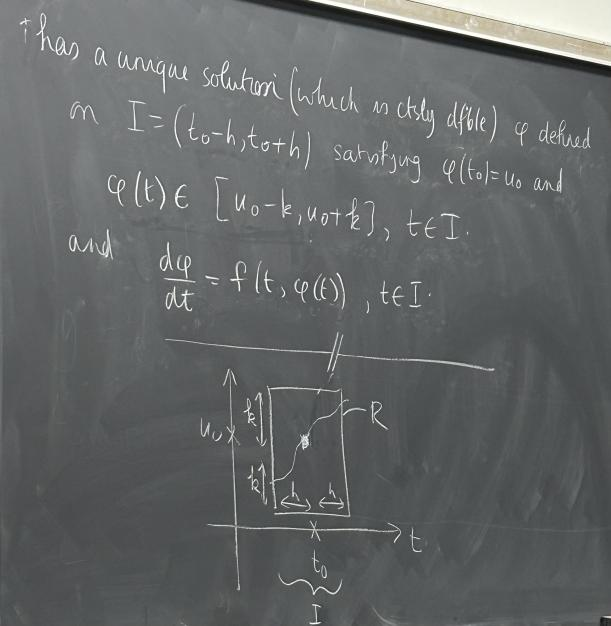
\includegraphics[width=0.6\textwidth]{Figures/lecture2/lec2-1.png}\]
    We would like to have $k$ small and $h$ large.
\end{remark}

\begin{remark}
    In this class, ``continuously differentiable" means the function is continuous, is differentiable, and the derivative is continuous.
\end{remark}

We need a couple of tools before proving Picard's Theorem:
\begin{enumerate}
    \item Let $C(I)$ be the space of bounded continuous functions on $I$ equipped with the $\ell^\infty$-norm
    \[||f|| = \sup_{t \in I} |f(t)|\]
    It has the following property:
    \begin{itemize}
        \item If there's a Cauchy sequenece $\{f_k\} \in C(I)$ such that $||f_k \to f_\ell|| \to 0$ as $k, \ell \to 0$, then there exists a limit $f \in C(I)$ such that
        \[\lim_{t \to \infty} ||f - f_t|| = 0\]
        (This is just saying that $\ell^\infty$ is complete). This is not too difficulty to prove, but we will omit it in class.
    \end{itemize}
    \item We need the following lemma
    \begin{lemma}
        Let $a < b$ and define the subset $E \subset C(I)$ by
        \[E = \{ f \in C(I) : a \leq f(t) \leq b, t \in I \}\]
        Suppose we have a sequence of functions $\{f_k\}$ in $E$ that converges to $f$, then $f \in E$.
    \end{lemma}

    \begin{remark}
        This just means that $E$ is a closed subspace of $C(I)$. Closed subspace of a complete metric space is a complete metric space.
    \end{remark}

    \begin{proof}
        Let $k \in \Nbb$, so $a \leq f_k(t) \leq b$ for all $t \in I$. For any $\epsilon > 0$, there exists $N$ such that
        \[|| f - f_n || < \epsilon \text{ for all $n > N$}\]
        \[\iff -\epsilon < f(t) - f_n(t) < \epsilon \text{ for all $n > N$}\]
        \[\iff a - \epsilon \leq f_n(t) - \epsilon < f(t) < f_n(t) + \epsilon \leq b + \epsilon\]
        This implies that $a + \epsilon < f(t) < b + \epsilon$ for all $t \in I$. Let $\epsilon \to 0$, we get that $f \in E$.
    \end{proof}
\end{enumerate}

\begin{proof}[Proof of Picard's Theorem]
    We seek a function $\varphi \in C(I)$, $\varphi(t) \in [u_0 - k, u_0 + k]$ for all $t \in I$, and
    \[\varphi(t) = u_0 + \int_{t_0}^t f(s, \varphi(s)) ds, \forall t \in I\]
    This is equivalent to saying $\frac{d\varphi}{dt} = f(t, \varphi(t))$ with initial conditions $\varphi(t_0) = u_0$ using the Fundamental Theorem of Calculus. In other words, we want to show $\varphi \in E$ with $a = u_0 - k$ and $b = u_0 + k$.\\

    Now, given an arbitrary function $\zeta \in E$, we define a new function
    \[\psi(t) = u_0 + \int_{t_0}^t f(s, \zeta(s)) ds, \forall t \in I\quad (\star)\]
    Observe that $\psi \in C(I)$. Clearly it is continuous, for boundedness, note that $(s, \zeta(s)) \in R$, we have that
    \[|\psi(t) - u_0| \leq |t - t_0| \sup_{s \in I} |f(s, \zeta(s))| \leq |t - t_0| M_0 \leq h M_0 \leq k\]
    where the last inequality comes from assumption of the theorem. Hence, $\psi(t) \in [u_0 - k, u_0 + k]$ for all $t \in I$. We conclude that $\psi \in E$.\\

    Consequently, $(\star)$ defines a mapping $T: E \to E$ by the rule $\psi = T(\zeta)$. Let $\zeta_1, \zeta_2 \in E$ and $\psi_1 = T(\zeta_1), \psi_2 = T(\zeta_2)$. Then
    \begin{align*}
        |\psi_1(t) - \psi_2(t)| &= |\int_{t_0}^t \{f(s, \zeta_1(s)) - f(s, \zeta_2(s))\} ds|\\
        &\leq |\int_{t_0}^t M_1 |\zeta_1(s) - \zeta_2(s)| | \tag*{Lipschitz in second variables}\\
        &\leq M_1 \sup_{s \in I} |\zeta_1(s) - \zeta_2(s)| |t - t_0|\\
        &= M_1 h ||\zeta_1 - \zeta_2||,\quad \forall t \in I
    \end{align*}
    Hence we have that
    \[||\psi_1 - \psi_2|| \leq M_1 h ||\zeta_1 - \zeta_2|| \quad (*)\]
    Now since $M_1 h < 1$ by assumption, the rest follows from \textbf{Banach's fixed point theorem}, but not everyone in the class knows this result! So we will proceed....\\

    Define a sequence $\{\varphi_n\}_{n=0}^\infty$ by the rule
    \[\varphi_0(t) = u_0, t \in I\]
    \[\varphi_{n+1} = T(\varphi_n), n = 0, 1, ....\]
    Hence, since $\varphi_0 \in E$ and since $T: E \to E$, we have a whole sequence in $E$. We will check this is a Cauchy sequence, let $m > n$, by Triangle's inequality and ``bootstrapping" this inequality, we have that
    \begin{align*}
        ||\varphi_m - \varphi_n|| &\leq ||\varphi_{m} - \varphi_{m-1}|| + ... + ||\varphi_{n+1} - \varphi_n||\\
        &\leq \sum_{\ell = 0}^\infty ||\varphi_{n + \ell + 1} - \varphi_{n + \ell}|| \\
        &\leq \sum_{\ell = 0}^\infty (M_1 h)^{n+\ell} ||\varphi_1 - \varphi_0||  \tag*{Using $(*)$}\\
        &= (M_1 h)^n  ||\varphi_1 - \varphi_0|| \sum_{\ell = 0}^\infty (M_1 h)^{\ell}\\
        &= (M_1 h)^n ||\varphi - \varphi_0|| \frac{1}{1 - M_1 h}
    \end{align*}
    Therefore, $||\varphi_m - \varphi_n|| \to 0$ as $n, m \to \infty$. This is a Cauchy seuqnece in $E$, so our lemma tells us that the limit $\varphi$ of this sequence is in $E$.\\

    Now, $||\varphi - T(\varphi)|| = ||\varphi - \varphi_{n+1} + \varphi_{n+1} - T(\varphi)|| \leq ||\varphi - \varphi_{n+1}|| + ||T(\varphi_n) - T(\varphi)|| \leq ||\varphi - \varphi_{n+1}|| + (M_1 h)||\varphi_n - \varphi||$ which tends to $0$ as $n \to \infty$, hence we verify that $\varphi$ is a fixed point of the integral equation earlier.\\

    For uniqueness, suppose there's another $\Tilde{\varphi} \in E$ such that $\Tilde{\varphi} = T(\Tilde{\varphi})$ but $\Tilde{\varphi} \neq \varphi$, then consider
    \begin{align*}
        ||\varphi - \Tilde{\varphi}|| &= ||T(\varphi) - T(\Tilde{\varphi})||\\
        &\leq M_1 h ||\varphi - \Tilde{\varphi}||\\
        &< ||\varphi - \Tilde{\varphi}|| \tag*{$M_1 h < 1$}
    \end{align*}
    which is a contradiction. Hence we conclude that $\varphi$ is unique.
\end{proof}

\begin{remark}
    This is a constructive argument to make $\varphi$. However, it is not so popular because the map $T$ tends to be difficult to compute.
\end{remark}

\newpage
\section{Lecture 3}

\subsection{More on Picard's Theorem}
Recall - last lecture, we proved Picard's Theorem:
\begin{theorem}[Picard's Theorem]
    Let $R = [t_0 - h, t_0 + h] \times [u_0 - k, u_0 + k]$ and suppose $f: R \to \Rbb$ is continuous with 
    \begin{enumerate}
        \item $|f(t, u)| \leq M_0$ for $(t, u) \in \Rbb$.
        \item Lipschitz with respect to the second variable, ie. for a fixed $t$
        \[|f(t, u) - f(t, v)| \leq M_1 |u - v|\]
        for $(t, u), (t, v) \in R$.
    \end{enumerate}
    If $M_0 h \leq k$ and $M_1 h < 1$ (so $h$ has to be sufficiently small), then the problem 
    \[\frac{du}{dt} = f(t, u), u(t_0) = u_0\]
    has a unique solution that is continuously differentiable $\varphi$ defined on $I = (t_0 - h, t_0 + h)$ (note that this is open) satisfying
    \begin{itemize}
        \item  $\varphi(t_0) = u_0$.
        \item $\varphi(t) \in [u_0 - k, u_0 + k]$ for all $t \in I$.
        \item $\frac{d\varphi}{dt} = f(t, \varphi(t))$ for all $t \in I$.
    \end{itemize}
\end{theorem}

What this theorem is really saying is that, given the initial condition $(t_0, u_0)$, there's some rectangle around the initial condition $(t_0, u_0)$: 
\[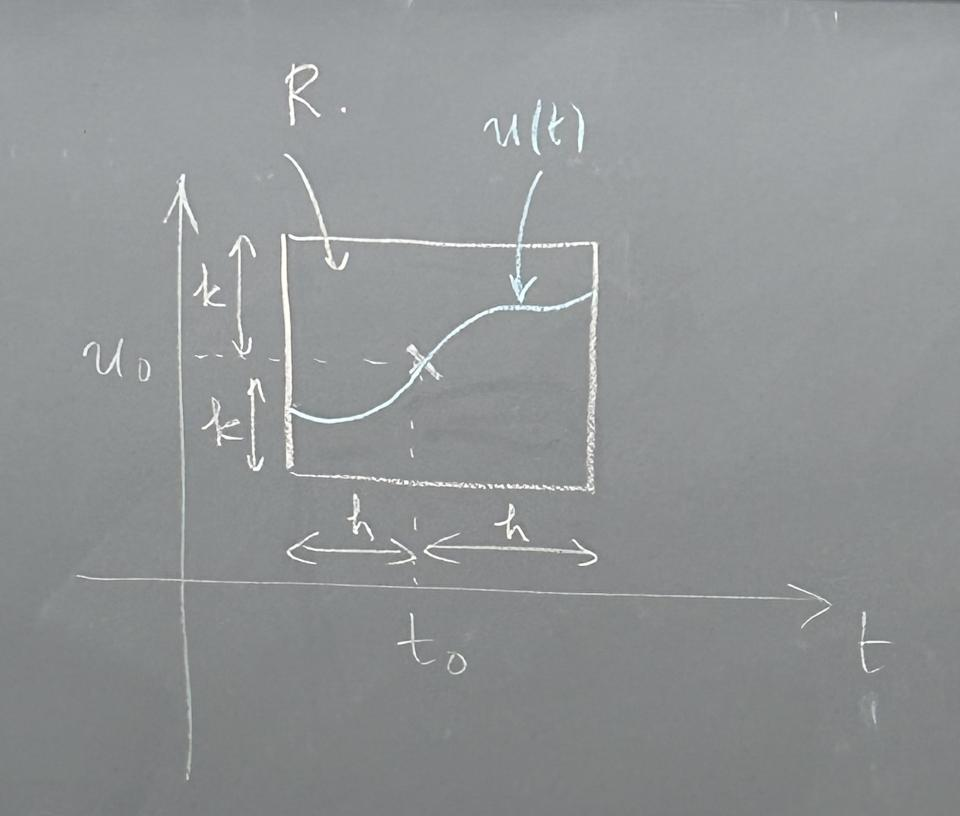
\includegraphics[width=0.6\textwidth]{Figures/lecture3/lec3-1}\]
such that $h$ has to be sufficiently small (recall $M_0 h \leq k$ and $M_1 h \leq k$), $t$ has to be sufficiently large, and thus $u(t)$ exists and is unique.

\begin{example}
    We will again consider a simple problem where $f(t, u) = -u^2$ and $u_0 = t_0 = 1$. We saw before that a solution exists only for $t > 0$. In other words, the global solution $u(t) = \frac{1}{t}$ is only defined to $t > 0$.\\

    Now, let's pretend the global solution is unknown and use Picard's theorem to give a local solution. Let's choose $r = [1 - h, 1 + h] \times [1 - k, 1 + k]$ where $h$ and $k$ are to be determined. Now, we check that
    \[|f(t, u)| = |-u^2| \leq (1 + k)^2 = M_0\]
    Also, we need to look at
    \[|f(t, u_1) - f(t, u_2)| = |u_1^2 - u_2^2| = |u_1 - u_2| |u_1 + u_2| \leq |u_1 - u_2| (|u_1| + |u_2|) \leq 2(1 + k) |u_1 - u_2|\]
    Hence we can take $M_1 = 2 (1 + k)$. We require $h$ and $k$ such that
    \[M_0 h \leq k \text{ and } M_1 h < 1\]
    This is equivalent to requiring that
    \[h \leq \frac{k}{(1 + k)^2} \text{ and } h < \frac{1}{2(1 + k)}\]
    We try to choose $h$ as large as possible to make the domain on which solutions exist as large as possible. This is comparing two curves:
\[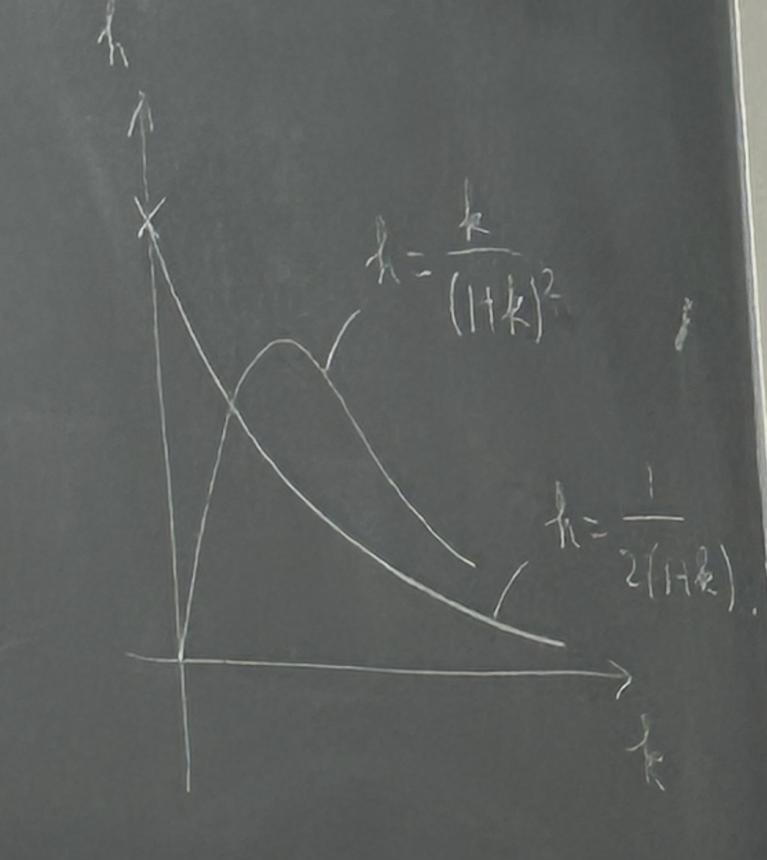
\includegraphics[width=0.4\textwidth]{Figures/lecture3/lec3-2}\]
    The largest value of $h$ is when the two curves intersect, which is at
    \[\frac{k}{(1 + k)^2} = \frac{1}{2(1 + k)} \iff k = 1\]
    Hence, the optimal choice is to take $k = 1$ and $h < 1/4$. Picard's Theorem then tells us that this initial valued problem has a unique solution on $R = [t_0 - h, t_0 + h] \times [u_0 - k, u_0 + k] = [\frac{3}{4}, \frac{5}{4}] \times [0, 2]$. The picture we should keep in mind is
\[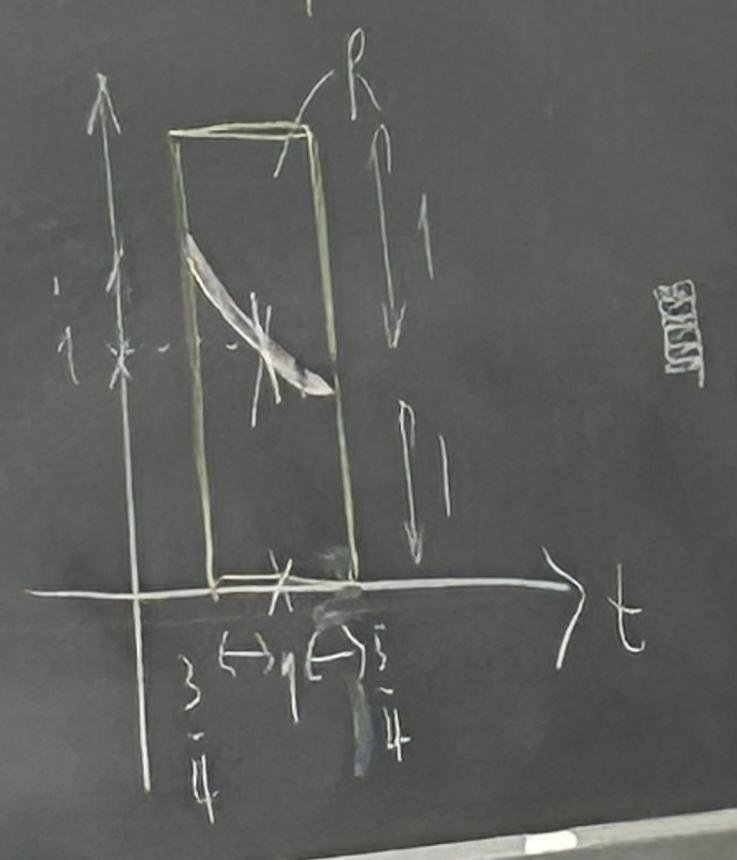
\includegraphics[width=0.4\textwidth]{Figures/lecture3/lec3-3}\]
\end{example}

\begin{question}
    Picard's Theorem told us about existence on $(3/4, 5/4)$, but we know that the solution exists on $(0, \infty)$. This result is not optimal. Can we try to extract some more information out of this? How to ``continue" (note that this is a pun)? 
\end{question}

Why don't we try to look at a point $(t_1, u_1)$ with $t_1 > t_0$, and make a new rectangle. Then we glue the rectangles together if the solutions agree. Then we try to do it for $t_2 > t_1$, etc.
\[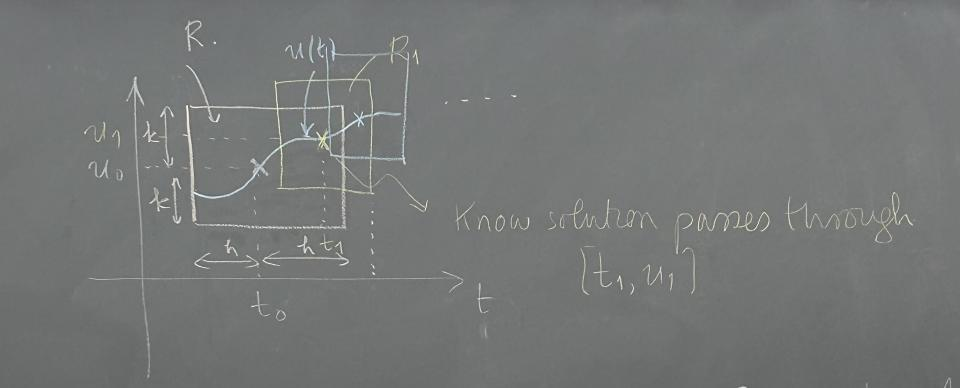
\includegraphics[width=0.8\textwidth]{Figures/lecture3/lec3-4}\]
Observe that the size of $I$ depends on $h$, which in turn only depends on $M_0$, $M_1$, and $k$, but not on the solution $\phi$ we constructed. This means that we can restart / continue the process of a new point $t_1$ such that $u(t_1) = u)1$, and extend to a new rectangle $R_1$.\\

We also notice that the new function $\varphi_1$ agrees with $\varphi$ on the common domain of definition by uniqueness of the solution. There is however one issue with this ``gluing method":
\begin{enumerate}
    \item What if the rectangle keeps shrinking until we eventually can't generate solutions to the entire interval?
\end{enumerate}

\begin{remark}
    If there's no limit on how large $h$ can be (ie. in the set up of the homework last week) in the case where we have a globally Lipschitz condition, we could always find the solution for the entire interval of definition.
\end{remark}

\begin{example}[Example Continued]
    Let's suppose that we start at a new point $t_0$ and $u_0 = \frac{1}{t_0}$, where $t_0$ could be $3/4$ or $5/4$ (from where we left off). Let $R = [t_0 - h, t_0 + h] \times [u_0 - k, u_0 + k]$ where $h$ and $k$ are to be determined again. Then, we have that
    \[|f(t, u)| = |u^2| \leq (u_0 + k)^2 = M_0\]
    \[|f(t, u_1) - f(t, u_2)| \leq |u_1 - u_2| 2(u_0 + k),\quad \text{ hence } M_1 = 2(u_0 + k)\]
    Now we require that $M_0 h \leq k$ and $M_1 h < 1$, which is equivalent to requiring
    \[h \leq \frac{k}{(u_0 + k)^2} \text{ and } h < \frac{1}{2(u_0 + k)}\]
    The optimal choice is when the two curves equal and is when $k = u_0$. Hence $h < \frac{1}{2(u_0 + k)} = \frac{1}{4(u_0)} = \frac{t_0}{4}$. Hence, by Picard's Theorem, the new (extended) interval is 
    \[(t_0 - h, t_0 + h) = (\frac{3 t_0}{4}, \frac{5 t_0}{4})\]
    which agrees with what we had when $t_0 = 1$. If we keep repeating this, we will get the interval after $n$ steps as
    \[(t_0 (\frac{3}{4})^n, t_0 (\frac{5}{4})^n)\]
    Hence, we get the interval $(0, \infty)$ as we take $n \to \infty$.
\end{example}

\begin{remark}
    Picard's theorem extends to systems of first order ODEs for, (ex. in the case of approximating Fisher's equation):
    \[\frac{d\Vec{u}}{dt} = \Vec{f}(t, \Vec{u}), \Vec{u} = (u_0, u_1, ..., u_{N-1}) \]
    where $\Vec{f}: \Rbb \times \Rbb^N \to \Rbb^N$ is bounded and continuous on some hyper-rectangle $R \subseteq \Rbb \times \Rbb^N$ and Lipschitz in all $\Vec{u}$-variables. The proof is almost exactly the same.\\

    Picard's theorem also extends to higher order ODEs:
    \[\frac{d^n u}{dt^n}(t) = f(t, u, \frac{du}{dt}, ..., \frac{d^{N-1} u}{dt^{N-1}}), N > 1\]
    We can change this into a system of first order ODEs as follows - we introduce new variables:
    \[u_0 = u, u_1 \coloneqq \frac{du}{dt}, ..., u_{N-1} \coloneqq \frac{d^{N-1}u}{dt^{N-1}} \]
    Let's set $\Vec{u} = [u_0, u_1, ..., u_{N-1}]$. This then gives us that
    \[\frac{d\Vec{u}}{dt} = [u_0', u_1', ..., u_{N-1}'] = [u_1, u_2, ..., u_{N-1}, \frac{d^N}{dt^N} u] = [u_1, u_2, ..., u_{N-1}, f]\]
    which we just talked about before.
\end{remark}

\subsection{Numerical Quadrature}
We are interested in IVPs of the form
\[\frac{du}{dt} = f(t, u)\]
using an numerical approach. However, even if $f(t, u)$ is independent of $u$, we still have an issue:\\

\begin{question}
Consider the set up
\[\frac{du}{dt}(t) = g(t), t > t_0 \text{ subject to } u(t_0) = u_0\]

We know the exact solution should be
\[u(t) = u_0 + \int_{t_0}^t g(s) ds,\quad t > t_0\]
However, in general this integral might be very difficult to compute analytically! We need to somehow approximate the integral.
\end{question}

Consider a new set up as follows - Suppose we solve a function $u(t)$ from $t = t_0$ to $t = T$,
\[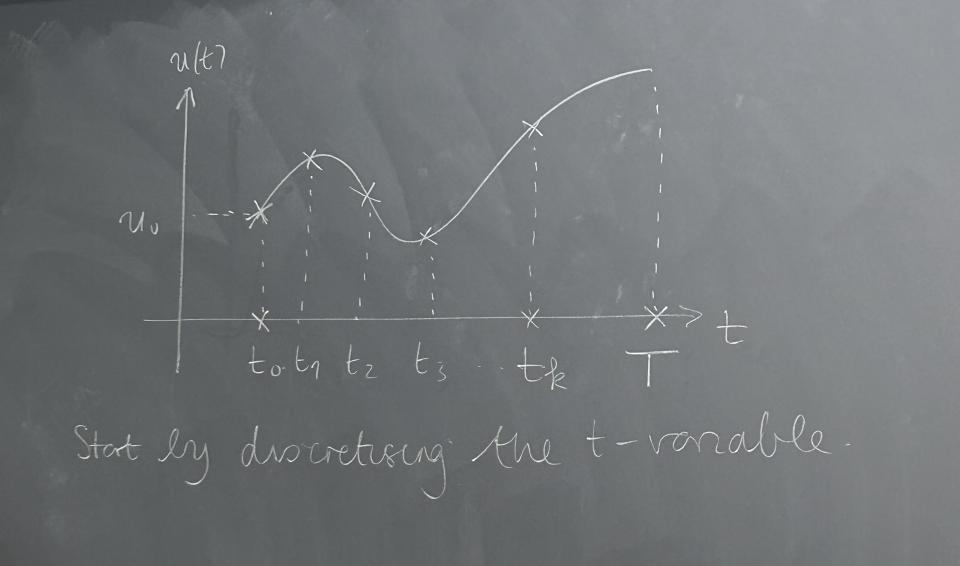
\includegraphics[width=0.5\linewidth]{Figures//lecture3/lec3-5.png}\]
We start by a uniform discretization of the $t$-variables. We define $t_k = t_0 + k h$ where $h = \frac{T - t_0}{n}$ and $n \in \Nbb$. We then try to compute the coordinates $(t_k, u(t_k))_{k = 0}^n$. We know that
\[u(t_1) = u_0 + \int_{t_0}^{t_1} g(s) ds\]
If $h = t_1 - t_0$ is small, then we should be able to approximate the integral ``well". For example, we could use the Trapezoidal rule,
\[\int_0^{h} g(s) ds \approx \frac{h}{2} \{g(0) + g(h)\}\]
This leads to a numerical algorithm:

\begin{tcolorbox}[standard jigsaw,opacityback=0]
\begin{algorithm}[H]
\caption{Trapezoidal Approximations}
\KwData{$u_0$ and $g$}
\KwResult{The tuples approximating $(t_k; u(t_k))_{k = 0}^n$}
1. Choose $n$ and set $h = \frac{T - t_0}{n}$\;
2. For $k = 1, 2, ...$, set $u_k = u_{k-1} + \frac{1}{2} h [g(t_{k-1}) + g(t_k)]$
\end{algorithm}
\end{tcolorbox}

There are however some issues
\begin{enumerate}
    \item How good are the results? We want to estimate $|u(t_k) - u_k|$.
    \item Does the method converge as $h \to 0$. In other words,
    \[\max_{0 \leq k \leq n} |u(t_k) - u_k| \to 0 \text{ as } h \to 0\]
    \item If it does converge, what conditions are on $g$? How fast does this converge? The speed should depend on $g$ and the choice of the quadrature rule.
\end{enumerate}

\begin{question}
    What other kinds of quadrature rule are possible?
\end{question}
\begin{itemize}
    \item Trapezoidal rule: $\int_0^h g(s) ds \approx \frac{h}{2} [g(0) + g(h)]$.
    \item Simpson's rule: $\int_0^h g(s) ds \approx \frac{h}{6} [g(0) + 4 g(\frac{h}{2}) + g(h)]$.
    \item Gauss-Legendre 2-point rule: $\int_0^h g(s) ds \approx \frac{h}{2}\{g(\xi_+) + g(\xi_-)\}$ where $\xi_\pm = \frac{h}{2}(1 \pm \frac{1}{\sqrt{3}})$.
    \item The Midpoint Rule (or Gauss-Legendre 1-point rule): $\int_0^h g(s) ds \approx h g(\frac{h}{2})$.
    \item Left-Hand Endpoint Rule: $\int_0^h g(s) ds \approx h g(0)$.
    \item ... and may others.
\end{itemize}
Any one of these could be used in our algorithm, so how do we know which to choose? There's no clear cut answer because it depends on what we are trying to do. We are interested in the following quantities:
\begin{itemize}
    \item Cost (Number of evaluations of $g$)
    \item Rate of convergence
    \item Accuracy
\end{itemize}

In order to answer these questions, we need rigorous error estimates on the quadrature rules. 
\begin{definition}
Assuming the function $g \in C[0, h]$ (it is continuous on $[0, h]$), let $I(g)$ be any of the quadrature rules, then the error function is defined as
\[g(s) \mapsto E(g) \coloneqq \int_0^h g(s) ds - I(g) \]
This is a linear functional $E$ in $\Hom(C[0, h], \Rbb)$. The point is that $E$ (and also $I$) acts on functions, so to be precise, we can write
\[E[t \mapsto g(t)] = \int_0^h g(s) ds - I[t \mapsto g(t)]\]
This will become important later.
\end{definition}

\begin{remark}
One time in the coffee room, the instructor was talking about Gaussian quadratures with his advisor. Roy Roberts heard and conversation and asked "What is the Gaussian quadrature"? Then the instructor's advisor explained. Roy Robert then asks - what happens when we have a function that is continuous nowhere? The instructor's advisor thought about it and then said "They don't usually come up in practice".
\end{remark}

\begin{example}
    Here are some examples of the error functional.
    \begin{enumerate}
        \item If the rule is the Trapezoidal rule, then
        \[E[t \mapsto g(t)] = \int_0^h g(s) ds - \frac{h}{2} [g(0) + g(h)]\]
        If $g(t) = 1$ is the constant function, then
        \[E[t \mapsto 1] = \int_0^h ds - \frac{h}{2}[1 + 1] = 0\]
        If $g(t) = t$, then
        \[E[t \mapsto t] = \int_0^h s ds - \frac{h}{2}[0 + h] = 0\]
        If $g(t) = t^2$, then
        \[E[t \mapsto t^2] = \int_0^h s^2 ds - \frac{h}{2}[0 + h^2] = -\frac{1}{6} h^3\]
    Since $E$ is a linear functional, we conclude that
    \[E[t \to p(t)] = 0 \quad \forall \text{p that is a polynomial of degree at most $1$.}\]

        \item If the rule is the midpoint rule, then
        \[E[t \mapsto g(t)] = \int_0^h g(s) ds - \frac{h}{2} [g(h/2)]\]
        We will again have that $E[t \mapsto 1] = 0$ and $E[t \mapsto t] = 0$. Now,
        \[E[t \mapsto t^2] = \frac{1}{12} h^{3}\]
        So $E[p] = 0$ for all linear polynomials $p$.

        \item If the rule is the two point Gauss-Legendre rule, then
        \[E[t \mapsto g(t)] = \int_0^h g(s) ds - \frac{h}{2} \{g(\xi_+) - g(\xi_-)\}\]
        where $\xi_{\pm} = \frac{h}{2} (1 \pm \frac{1}{\sqrt{3}})$. In this case we still have $E[t \mapsto 1] = 0$ and $E[t \mapsto t] = 0$. Furthermore, $E[t \mapsto t^2] = 0$ and in fact even $E[t \mapsto t^3] = 0$. However, $E[t \mapsto t^4] \neq 0$. In fact, we have that $E[p] \equiv 0$ for all polynomials $p$ with degree less than or equal to $3$. In fact, this the maximal precision, no 2-point rule can eliminate more polynomials than the two point Gauss-Legendre rule.\\

        In general, given $E[t \mapsto g(t)]$, we note that
        \[E[t \mapsto g(t)] = E[t \mapsto g(t) - p_3(t)], \forall p_3 \in \Pbb_3\]
        (here $\Pbb_n$ means all polynomials with degree less than or equal to $n$). Hence, if we could find a good approximation of $g(t)$ using cubics, we could get a good error!
    \end{enumerate}
\end{example}

\begin{conjecture}
    If $E[p] \equiv 0$ for all $p \in \Pbb_n$, then for ``reasonable $g$", $E[g]$ should be small and should ``be better" as $n$ increases. 
\end{conjecture}

This will be formalized and will be known as the \textbf{Peano Kernel Theorem}.

\newpage
\section{Lecture 4}

\subsection{Peano Kernel Theorem}

We are developing and analyzing rates for
\[\int_0^h g(t) dt \simeq \text{ Linear combination of values of $f$.}\]
e.g. we have the Trapezoidal Rule, 
\[\int_0^h g(t) dt \simeq \frac{h}{2} [g(0) + g(h)]\]

\begin{question}
    How accurate is this rule? How to compute the rules?
\end{question}

This led us to define the error functional $E: C[0, h] \to \Rbb$ that takes a continuous function on $[0, h]$ by the rule
\[E(g) = \int_0^h g(t) dt - \frac{h}{2} [g(0) + g(h)]\]
Strictly speaking, this is being applied to the function $t \mapsto g(t)$, so we should really think of $E(g)$ as $E[t \mapsto g(t)]$.\\

What we found was that for this (and other) rules, we have the property that
\[E[t \mapsto p(t)] = 0 \quad \forall p \in \Pbb_n\]
for some $n$. This led us with an idea:

\begin{idea}
Try to estimate $E(g)$, where $g$ is a smooth function, by writing
\[E(g) = E(g - p) \quad \forall p \in \Pbb_n\]
We suspect that this should be ``small", the precise definition of smallness is yet to be defined. If we trake $p(t)$ to be a good approximation of $g(t)$, then $g - p$ should be ``small". Can we make this rigorous?
\end{idea}

\begin{remark}
    Being a good researcher at maths isn't being a good person at taking exams. The hardest part of mathematics is what to prove, rather than how to prove it. Sometimes we make the initial thing to prove easier by adding more and more constraints, we want to refine the statement we want to prove from the initial idea. Therefore, the initial intuition is very important, and the rest is trying to make this intuition rigorous.
\end{remark}

Let's start with Taylor's Theorem. The Maclaurin series tells us that for large $n$
\[g(t) \approx \sum_{k = 0}^n \frac{t^k}{k!} g^{(k)}(0)\]

We want to bound the error by looking at the reimander term:
\begin{theorem}[Taylor's Theorem] The remainder term may be expressed as, after successive integration by parts,
    \[g(t) = \sum_{k = 0}^n \frac{t^k}{k!} g^{(k)}(0) + \frac{1}{n!} \int_0^t (t - s)^m g^{(n+1)}(s) ds, \quad t \in [0, h] \]
    Let's call $p_n(t) = \sum_{k = 0}^n \frac{t^k}{k!} g^{(k)}(0)$.
\end{theorem}

Let define the \textbf{truncated power function}) as
\[(t - s)^n_+ = \begin{cases}
    (t - s)^n, \text{ if $t \geq s$}\\
    0, \text{ if $t < s$}
\end{cases}\]

Then we can write
\[g(t) = p_n(t) + \frac{1}{n!} \int_0^h (t - s)^m_+ g^{(n+1)}(s) ds\]
The beauty is now the integral's range is independent of $t$. Let's try to apply the error functional to both side, then
\begin{align*}
    E[t \mapsto g(t)] &= E[t \to p_n(t)] + \frac{1}{n!} \int_0^h E[t \mapsto (t - s)^m_+] g^{(n+1)}(s) ds \tag*{Fubini's Theorem}\\
    &= \frac{1}{n!} \int_0^h E[t \mapsto (t - s)^m_+] g^{(n+1)}(s) ds \tag*{By Hypothesis, $E[t to p_n(t)] = 0$}
\end{align*}

Let's define $s \mapsto K(s) = E[t \mapsto (t - s)^m_+] \in \Rbb$, which is a real number that has no $t$-variables anymore. We call $K(s)$ the \textbf{kernel function}. This leads to a theorem:

\begin{theorem}[Peano Kernel Theorem]
    Let $E: C[0, h] \to \Rbb$ be a linear functional which commutes with integrals such that $E(p) \equiv 0$ for all $p \in \Pbb_n$ for some $n \in \Zbb_{\geq 0}$. If $g \in C^{n+1}([0, h])$, then 
    \[E[t \mapsto g(t)] = \frac{1}{n!} \int_0^h K(s) g^{(n+1)}(s) ds\]
    where the construction of $K(s) = E[t \mapsto (t - s)^m_+]$ is the kernel. Here, $C^{n+1}$ means $(n+1)$-th times continuously differentiable.
\end{theorem}

Consequenetly, we get the following error bounds:
\begin{corollary}
Let $E: C[0, h] \to \Rbb$ be a linear functional as before and $g \in C^{n+1}([0, h])$, then
\begin{itemize}
    \item $|E(g)| \leq \frac{1}{n!} \int_0^h |K(s)| ds \cdot \max_{0 \leq t \leq h} |g^{n+1}(t)|$.
    \item $|E(g)| \leq \frac{1}{n!} \max_{0 \leq s \leq h} |K(s) \cdot \int_0^h |g^{n+1}(s)| ds$.
    \item $|E(g)| \leq \frac{1}{n!} \sqrt{\int_0^h K(s)^2 ds} \cdot \sqrt{\int_0^h g^{(n+1)}(s)^2 ds}$.
    \item Pick any of your favorite Holder's Inequality.
\end{itemize}
\end{corollary}

\begin{remark}
Peano's Kernel Theorem is not usually covered in many numerical analysis, but it is covered in \textit{Interpolations and Approximation} by P. J. Davis, who used to be a Brown professor here. The instructor actually has his office now. The instructor owns the book ever since $1988$ with the author's signature. The instructor lent the book to someone, and now it is lost forever now...
\end{remark}

\begin{example}
    Here are some applications of the theorem: For the Trapezoidal rule, we know that $E(p) \equiv 0$ for all $p \in \Pbb_1$, and we show that $E[t \mapsto t^3] = -\frac{1}{6}h^3 \neq 0$, so applying the Peano kernel theorem with $n = 1$, we have that for $s \in [0, h]$,
       \begin{align*}
           K(s) &= \frac{1}{1!} E[t \mapsto (t-s)^1_+]\\
           &= \int_0^h (t - s)_+ dt - \frac{h}{2}[(h - s)_+ - (0 - s)_+]\\
           &= \int_s^h (t - s) dt - \frac{h}{2}\{(h - s) + 0\} \tag*{$(t - s)_+$ is non-zero only when $t > s$}\\
           &= \frac{1}{2} (h - s)^2 - \frac{1}{2} h(h-s)\\
           &= -\frac{1}{2} (h-s)s
       \end{align*}
       Observe that $K(s)$ is just a function of $s$, nothing special. We can draw a picture of it:
       \[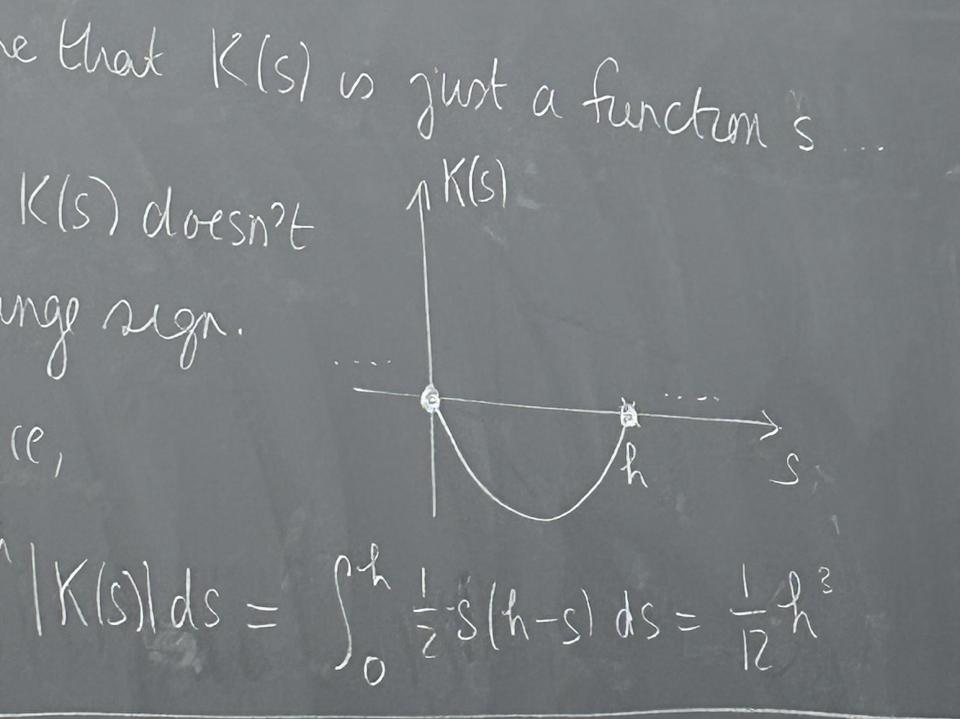
\includegraphics[width=0.6\textwidth]{Figures/lecture4/lec4-1.png}\]
       Boudning the kernel we note that
       \[\int_0^h |K(s)| ds = \int^h_0 \frac{1}{2} s(h - s) ds = \frac{1}{12} h^3\]
       Hence we have that
       \[|\int_0^h g(s) ds - \frac{h}{2} \{g(0) + g(h)\}| \leq \frac{1}{12} h^3 \max_{0 \leq t \leq h} |g''(t)|\]
\begin{question}
    Can this be improved? (e.g. smaller constants or bigger powers of $h$).
\end{question}
No, we just need to exhibit a function such that they are equal on both sides, this holds as an equality when $g(t) = t^2$.
\end{example}

We only cared about $K(s)$ for $s \in [0, h]$, but if we try to extend $s$ beyond this range... What would happen? Suppose $s < 0$, then
    \begin{align*}
        K(s) &= \int_0^h (t - s)_+ dt - \frac{h}{2} \{(h - s)_+ - (0 - s)_+\}\\
        &= \int_0^h (t - s) dt - \frac{h}{2} \{(h - s) + (-s)\}\\
        &= [\frac{1}{2} (t - s)^2]_0^h - \frac{1}{2} h^2 + s\\
        &= \frac{1}{2} (h - s)^2  - \frac{1}{2} s^2 - \frac{1}{2} h^2 + s\\
        &= 0 \tag*{As expected}
    \end{align*}
In general, we have that
\begin{proposition}
    $K(s) = 0$ for all $s < 0$ and $s > h$.
\end{proposition}

\begin{proof}
    If $s < 0$ and $t \in [0, h]$, then $(t - s)_+^n = (t - s)^n$, so in this case
    \[K(s) = E[t \mapsto (t - s)^n] = 0 \text{ as $(t - s)^n \in \Pbb_n$}.\]
    If $s > h$ and $t \in [0, h]$, then $(t - s)_+^n = 0$, so
    \[K(s) = E[t \mapsto 0] = 0.\]
    This concludes the proof.
\end{proof}

Let's try another example,
\begin{example}[Left hand endpoint rule]
    Let's consider
    \[E(g) = \int_0^h g(t) dt - h g(0)\]
    In this case, we have that
    \[E(t \mapsto 1) = \int_0^h dt - h = 0\]
    \[E(t \mapsto t) = \int_0^h t dt - h \cdot 0 = \frac{1}{2} h^2 \neq 0\]
    Hence we have that $E(p) = 0$ for all $p \in \Pbb_0$. In this case the Peano Kernel is 
    \[K(s) = \frac{1}{0!} E[t \mapsto (t - s)_+^0] = \int_0^h (t - s)^0_+ dt - h (0 - s)_+^0 = \int_s^h 1 dt - 0 = h - s \]
    This is just the function:
    \[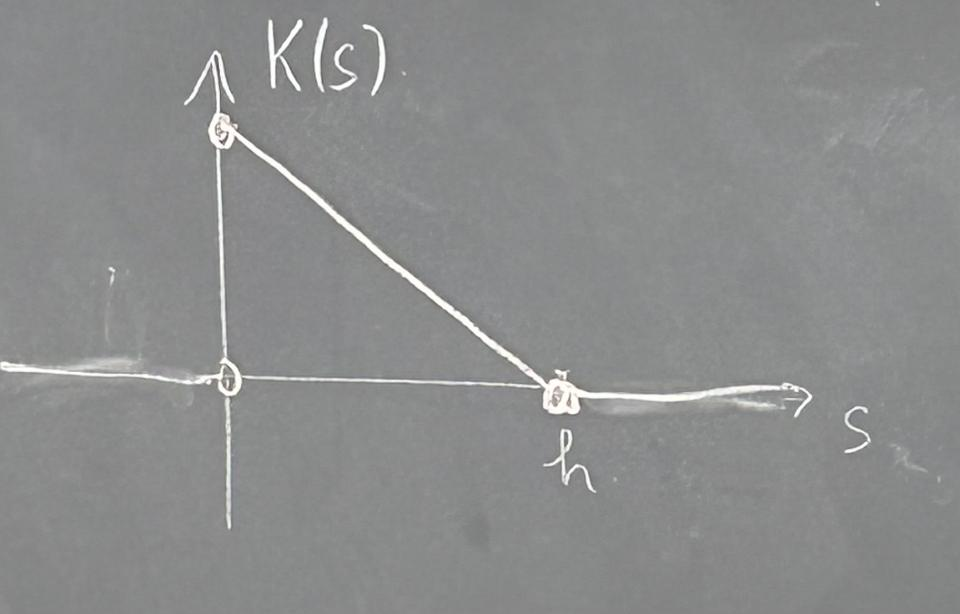
\includegraphics[width=0.6\textwidth]{Figures/lecture4/lec4-2.png}\]
    Note that $K(s)$ does not change sign so
    \[\int_0^h |K(s)| ds = \int_0^h (h - s) ds = \frac{1}{2} h^2\]
    Hence we have that
    \[|\int_0^h g(s) ds - h g(0)| \leq \frac{1}{2} h^2 \max_{0 \leq t \leq h} |g'(t)|\]
    This can't be improved, just pick $g(t) = t$ and the above expression will hold as an equality.
\end{example}

Let's try another example,
\begin{example}[Midpoint rule]
    Let's consider
    \[E(g) = \int_0^h g(t) dt - h g(\frac{h}{2})\]
    We have that $E(p) = 0$ for all $p \in \Pbb_1$ with $E[t \mapsto t^2] = \frac{h^3}{12}$. We take $n = 1$ and let $s \in [0, h]$, then
\begin{align*}
    K(s) &= \frac{1}{1!} E[t \mapsto (t - s)_+]\\
    &= \int_s^h (t - s) dt - h (\frac{1}{2} h - s)_+\\
    &= \begin{cases}
        \frac{1}{2}(h - s)^2 - h(\frac{1}{2} h  - s), \quad s \leq \frac{1}{2}h\\
        \frac{1}{2}(h - s)^2,\quad s > \frac{1}{2}h
    \end{cases}\\
    &= \begin{cases}
        \frac{1}{2}s^2,\quad s \leq \frac{1}{2}\\
        \frac{1}{2}(h-s)^2,\quad s > \frac{1}{2}
    \end{cases}
\end{align*}
We have the picture
\[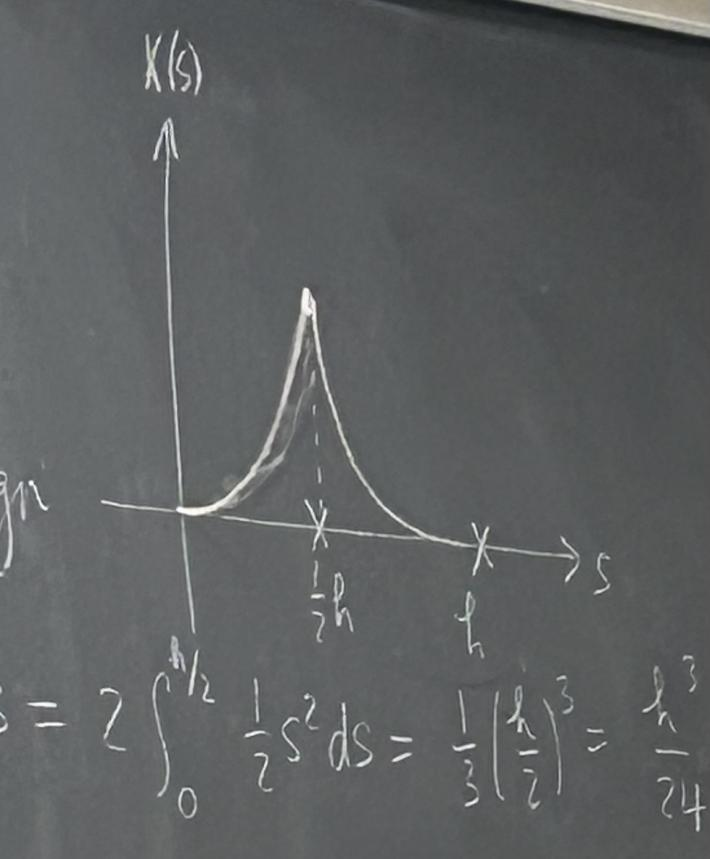
\includegraphics[width=0.4\textwidth]{Figures/lecture4/lec4-3.png}\]
Note that $K(s)$ has a single sign, so
\begin{align*}
    \int_0^h |K(s)| ds &= \int_0^h K(s) ds\\
    &= 2 \int_0^{h/2} \frac{1}{2} s^2 ds\\
    &= \frac{1}{3} (\frac{h}{2})^3\\
    &= \frac{h^3}{24}
\end{align*}
Hence we have that
\[|\int_0^h g(t) dt - h g(\frac{h}{2})| \leq \frac{h^2}{24} \max_{0 \leq t \leq h} |g''(t)|\]
and the maximum is achieved with some choice of functions $g(t) = t^2$.
\end{example}

\begin{question}
    By these 3 previous examples, we want to ask:
    \begin{enumerate}
        \item Is $K(S)$ always single signed?
        \item What if $g$ does not belong to $C^{n+1}[0, h]$?
    \end{enumerate}
\end{question}

Let's start with Question 2, we know that if $E(p) \equiv 0$ for all $p \in \Pbb_n$, then the error may be written as
\[E(g) = \int_0^h K(s) g^{(n+1)}(s) ds\]
Suppose we only know that $g \in C^{n}[0, h]$, then the formula above makes no sense. Why don't we instead consider $p \in \Pbb_{n-1} \subseteq \Pbb_n$? Hence, we pretend that we only know $E(p) \equiv 0$ for all $p \in \Pbb_{n-1}$.

\begin{example}[Kernal is not single signed]
Let's try this on the midpoint rule if $g \in C^1[0, h]$ (previously assumed it's in $C^2$), then $E(p) \equiv 0$ for all $p \in \Pbb_0$.\\

In this case, we denote the kernel associated with $n = 0$ as $K_0$ and
\[K_0(s) = \frac{1}{0!} E[t \mapsto (t - s)_+^0] = \int_s^h dt = \int_s^h 1 dt - h(\frac{h}{2} - s)_+^0 = \begin{cases}
    (h-s)-h,\quad s < \frac{h}{2}\\
    h-s,\quad s \geq \frac{h}{2}
\end{cases} \]
Hence we have that
\[K_0(s) = \begin{cases}
    -s, \quad s < \frac{h}{2}\\
    h-s, s \geq \frac{h}{2}
\end{cases}\]
The graph looks like:
\[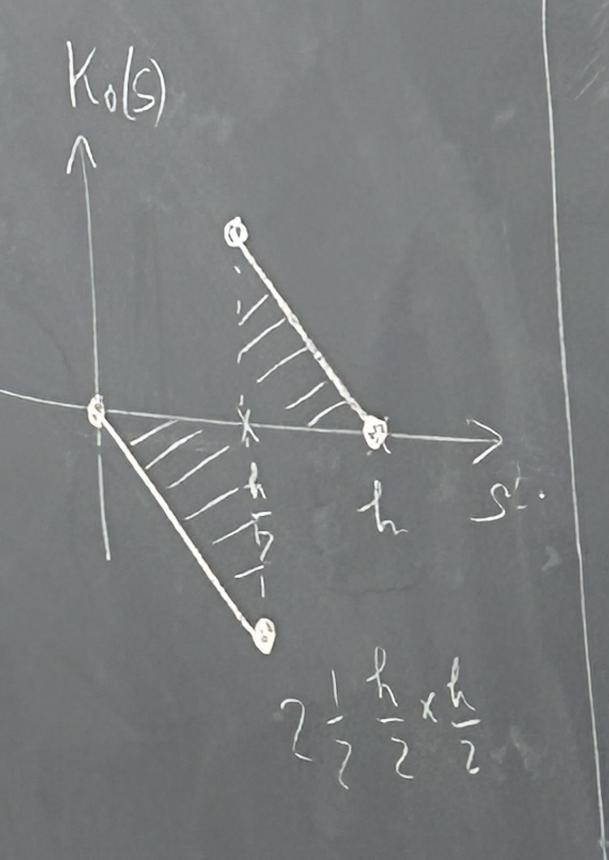
\includegraphics[width=0.4\textwidth]{Figures/lecture4/lec4-4.png}\]
This is NOT a single signed function! In this case, we have that
\[\int_0^h |K_0(s)| ds  = \frac{h^2}{4}\]
So we obtained that
\[|\int_0^h g(s) ds - h g(\frac{h}{2})| \leq \frac{h^2}{4} \max_{0 \leq t \leq h} |g'(t)|\]
Sometimes it might actually be better to only use one derivative instead of two, for example consider $g(t) = e^{-1000t}$, the error bound for a single derivative is better than that of a double derivative.
\end{example}

\begin{remark}
    P. D. Lax and Louis Nivenberg. One time Nivenberg was interviewed by a popular magazine and was asked ``What's one reason you would attribute to your success in mathematics?" Nivenberg thought about it and answered: ``Whenever I get stuck, I always try to do integration by parts." Nivenberg later admitted that he was actually being half-serious while answering this.
\end{remark}

We see now that $K(s)$ is not always single-signed, but in a lot of cases it is. So much so that we want show the following corollary.
\begin{corollary}
    Suppose $E(p) \equiv 0$ for all $p \in \Pbb_n$ and that 
    \[E[t \mapsto (t - s)^n_+] \text{ is single signed for $s \in [0, h]$.}\]
    If $g \in C^{n+1}[0, h]$, then there exists some $\xi \in (0, h)$ such that
    \[E(g) = \frac{1}{(n+1)!} E[t \mapsto t^{n+1}] g^{(n+1)}(\xi)\]
\end{corollary}

\begin{proof}
    By Peano Kernel Theorem, we have that 
    \begin{align*}
        E(g) &= \int_0^h K(s) g^{(n+1)}(s) ds
    \end{align*}
    where $K(s)$ is single-signed, without loss we will assume that $K(s) \geq 0$. Let's then consider
    \[Q = [\int_0^h K(s) g^{(n+1)}(s) ds] / [\int_0^h K(s) ds]\]
    Note that the denominator is zero only when $K(s)$ is zero almost everywhere (since $K(s)$ has signle sign), which are degenerate cases we ignore. Now, we have that
    \[\min_{0 \leq t \leq h} g^{(n+1)}(t) \leq Q = \frac{\int_0^h K(s) g^{(n+1)}(s) ds}{\int_0^h K(s) ds} \leq \max_{0 \leq t \leq h} g^{(n+1)}(t)\]
    This means that $Q$ is in the range of the function $g^{(n+1)}(t)$ for $t \in [0, h]$. By the intermediate value theorem, there exists a point $\xi \in (0, h)$ such that
    \[Q = g^{(n+1)}(\xi)\]
    Hence, $E(g) = \int_0^h K(s) g^{(n+1)}(s) ds = Q \int_0^h K(s) ds = g^{(n+1)}(\xi) \int_0^h K(s) ds$. This is true for all $g \in C^{n+1}[0, h]$. Let's choose $g(t) = t^{n+1}$, and the result reads
    \[E(t^{n+1}) = \left(\int_0^h K(s) ds\right) g^{(n+1)}(\xi) = \left(\int_0^h K(s) ds\right) (n+1)! \]
    Hence we have that
    \[\int_0^h K(s) ds = \frac{1}{(n+1)!} E(t^{n+1})\]
    Hence, we conclude that
    \[E(g) = \frac{1}{(n+1)!} E(t^{n+1}) g^{(n+1)}(\xi)\]
\end{proof}

\begin{example}Applying this corollary:
\begin{enumerate}
    \item For the trapezoidal rule, we have that
    \[E(t \mapsto t^2) = -\frac{1}{6} h^2 \text{ and } K(s) \leq 0\]
    Hence, there exists $\xi \in (0, h)$ such that
    \[\int_0^h g(t) dt - \frac{h}{2} \{g(0) + g(h)\} = \frac{1}{2!} \frac{h^3}{6} g''(\xi) = -\frac{h^3}{12} g''(\xi)\]
    \item For the midpoint room, we have that
    \[E(t \mapsto t^2) = \frac{h^3}{12} \text{ and } K(s) \geq 0\]
    So there exists $\xi \in (0, h)$ such that
    \[\int_0^h g(t) ds - h g(\frac{h}{2}) = \frac{1}{24} h^3 g''(\xi)\]
    \item For the left hand endpoitn rule, we have that
    \[E(t \mapsto t) = \frac{1}{2} h^2 \text{ and } K(s) \geq 0\]
    Sot here exists $\xi \in (0, h)$, we have that
    \[\int_0^h g(t) dt - h g(0) = \frac{h^2}{2} g'(\xi)\]
\end{enumerate}
    Notice that $(1)$ to $(3)$ here immediately give the previous bounds for $|E(g)|$ obtained earlier. However, these results in this example are strongr in the sense that they are equalities (so they cannot be improved) and they gave the sign of the error.
\end{example}

\subsection{Interlude (Mathematical Candy / New Rules from Old)}
 We showed that there exist $\xi_T, \xi_M$ such that:
 \begin{itemize}
     \item For the trapezoidal rule (T),
     \[E_T(g) \coloneqq \int_0^h g(t) dt - \frac{h}{2}\{g(0) + g(h)\} = -\frac{h^3}{12} g''(\xi_T)\]
     \item For the midpoint rule (M),
     \[E_M(g) \coloneqq \int_0^h g(t) dt - h g(\frac{h}{2}) = \frac{h^3}{24} g''(\xi_M) \]
 \end{itemize}

\begin{question}
Can we exploit the fact that the different signs of error can be used to create a new rule with higher accuracy?    
\end{question}

Let's try to construct a new rule,
\[\Tilde{I}(g) = \alpha_M h g(\frac{h}{2}) + \alpha_T \frac{h}{2} \{g(0) + g(h)\}, \text{ for $\alpha_T, \alpha_M$ t.b.d}\]
So we then define the new error as
\[\Tilde{E}(g) = \int_0^h g(t) dt - \Tilde{I}(g)\]

Then we compute that
\[\Tilde{E}(t \mapsto 1) = h - h \alpha_T - h \alpha_M \]
If we want this to be $0$, we need that $\alpha_T + \alpha_M = 1$. Hence, we have that
\[\Tilde{E}(g) = (\alpha_T + \alpha_M) \int_0^h g(t) dt - \Tilde{I}(g) = \alpha_T E_T(g) + \alpha_M E_M(g) \]
Now, for linear terms
\[\Tilde{E}(t \mapsto t) = \alpha_T E_T(t \mapsto t) + \alpha_M E_M(t \mapsto t) = \alpha_T(0) + \alpha_M(0) = 0\]
For the quadratic term, we have that
\[\Tilde{E}(t \mapsto t^2) = -\frac{h^3}{6} \alpha_T + \frac{h^3}{12} \alpha_M\]
If we want this to be $0$, then we are solving the linear system
\[\begin{cases}
    \alpha_M + \alpha_T = 1\\
    \alpha_M = 2\alpha_T
\end{cases}\]
This tells us that
\[\alpha_M = \frac{2}{3} \text{ and } \alpha_T = \frac{1}{3}\]

Hence, the new rule is
\[\Tilde{I}(g) = \frac{2}{3} h g(\frac{h}{2}) + \frac{1}{3} \frac{h}{2} \{g(0) + g(h)\} = \frac{h}{6} \{g(0) + 4 g(\frac{h}{2}) + g(h)\}\]
This is just \textbf{Simpson's Rule}!\\

We could repeat this on Simpson's rule and another rule with an opposite sign, then we can use this to make other rules. This will be very important when we use them to solve ODEs.

\newpage
\section{Lecture 5}

\subsection{Composite Quadrature Rule}

We are interested in solving the IVP
\[\frac{dg}{dt}(t) = g(t), u(t_0) = u_0\]
for g ``reasonable". We had an algorithm given by, for example the trapezoidal rule,
\[u_{k+1} = u_k + \frac{h}{2} [g(t_k) + g(t_{k+1})], k \geq 0, \quad (X)\]
, where $t_k = kh$. Note that we can plug in any other quadrature.

\begin{question}
    Can we estimate the error and/or prove convergence?
\end{question}

Indeed, the error at the $k$-th step is
\begin{align*}
    u(t_{k+1}) - u_{k+1} &= \{ u(tk) + \int_{t_k}^{t_{k + 1}} g(s) ds\} - \{u_k + \frac{h}{2} [g(t_k) + g(t_{k+1})]\}\\
    &= (u(t_k) - u_k) + \{\int_{t_k}^{t_{k+1}} g(s) ds - \frac{h}{2} [g(t_k) + g(t_{k+1})\}\\
    &= (u(t_k) - u_k) + \frac{1}{12} h^3 g''(\xi_k) \tag*{Peano's Kenrel Theorem for Trapezoidal Rule, $\xi_k \in (t_k, t_{k+1})$}
\end{align*}
We also note that $u(t_0) - u_0 = 0$. We can extract the error out of this telescoping sum for $k = 0, 1, ..., n-1$ and see that
\begin{align*}
    u(t_n) - u_n &= \sum_{k=0}^{n-1} \frac{1}{12} h^3 g''(\xi_k)\\
    &= \frac{1}{12}(nh) h^2 \{\frac{1}{n} \sum_{k = 0} g''(\xi_k)\}\\
    &= \frac{1}{12} (t_n - t_0) h^2 \{\frac{1}{n} \sum_{k = 0} g''(\xi_k)\}
\end{align*}
Note that
\[\min_{t_0 \leq t \leq t_n} g''(t) \leq \frac{1}{n} \sum_{k = 0}^{n-1} g''(\xi) \leq \max_{t_0 \leq t \leq t_n} g''(t)\]
Hence, by the Intermediate Value Theorem, there exists $\tau_n \in (t_0, t_n)$ such that $\frac{1}{n} \sum_{k = 0}^{n-1} g''(\xi) = g''(\tau_n)$. Hence
\begin{align*}
    u(t_n) - u_n &= \frac{1}{12} (t_n - t_0) h^2 g''(\tau_n)
\end{align*}

\begin{remark}[Digression to Gauss-Legendre Rule]
For the $n+1$-point Gauss-Legendre rule, we have the polynomial
$$\varphi(t) = (t - \xi_0) (t - \xi_1) ... (t - \xi_n)$$
which we seek to satisfy
$\int_a^b \varphi(t) p(t) dt = 0$ for all $p \in \Pbb_{2n - 1}$. This comes down to finding a polynomial that's orthogonal to all polynomials of degree less than or equal to $2n - 1$. We can do this using Gram-Schmidt, then the roots of $\varphi(t)$ are the nodes of the Gauss-Legendre Rule. This is a non-linear problem in the sense that solving for the roots of $\varphi(t)$ is non-linear.
\end{remark}

More generally, we have the following theorem
\begin{theorem}
    Let $\{t_k, u_k\}_{k = 0}^N$ be defined by Algorithm $(X)$ based on a quadrature rule $Q$ that has remainder 
    \[\int_0^h g(s) ds - Q_{[0, h]}(g) = C h^{r+1} g^{r)}(\xi), \xi \in (0, h)\]
    Then, there exists $\tau_n \in (t_0, t_n)$ such that
    \[u(t_n) - u_n = \Tilde{C} h^r (t_n - t_0) g^{(r)}(\tau_n)\]
    for $n = 1, 2, ..., N$.
\end{theorem}

\begin{proof}
    Similar to above.
\end{proof}

\begin{corollary}
From the theorem above, we obtain the corollaries:
\begin{enumerate}
    \item If $g \in C^{r}[t_0, t_n]$, then $u(t_n) - u_n = O(h^r)$ which tends to $0$ as $h \to 0$. Hence, Algorithm $(X)$ is convergent as a rate of $O(h^r)$.
    \item If we choose $n = N$ from Theorem and use the Trapezoidal rule, then with $t_N = b$ and $t_0 = a$, we get
    \[ \int_a^b g(s) ds - h \sum_{k=0}^{N} {''} g(t_k) = \frac{1}{12}(b-a) h^2 g''(\tau), \tau \in (a, b) \]
    The notation $\sum''$ indicates that the first and final terms are halved. Pictorially, we are doing
\[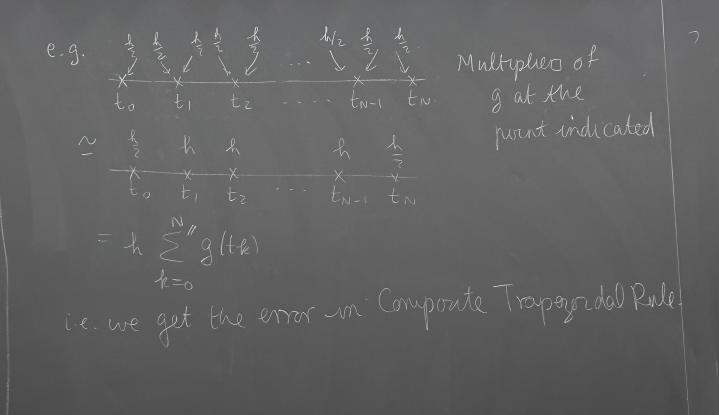
\includegraphics[width=0.6\linewidth]{Figures//lecture5/lec5-1.png}\]
    In other words, we get the error in Composite Trapezoidal Rule.
\end{enumerate}
\end{corollary}

\begin{example}
    Let's try to approximate $\int_0^1 \frac{4}{1 + t^2} dt = \pi$. Let's try to use rules with more and more points. Doing them in a program, we get that

    \begin{center}
\begin{tabular}{||c c c||} 
 \hline
 N & Error for Trapezoid & Error for Simpsion \\ [0.5ex] 
 \hline\hline
 1 & 0.2 & 0.00850095 \\ 
 \hline
 2 & 0.102353 & 0.000626097  \\
 \hline
 4 & 0.0246784 & 4.8676(-5) \\
 \hline
  8 & 0.006206 & 3.02298(-6) \\
 \hline
  16 & 0.001560 & 1.91704...(-7) \\
 \hline
 32 & 0.0003897 & 1.1959...(-8) \\ 
  \hline
 $\infty$ & $O(h^2)$ & $O(h^4)$ \\ [1ex] 
 \hline
\end{tabular}
\end{center}

We get $h^2$ and $h^4$ by fitting a line to the data. WHat you do is to assume that
\[E_n = C n^{-\alpha}, \text{ for $C, \alpha$ t.b.d}\]
Then we take logarithm to get
\[\log E_n = \log C - \alpha \log n\]
We then do a plot of $\log E_n$ against $\log n$ (which is linear with slope $-\alpha$):
\[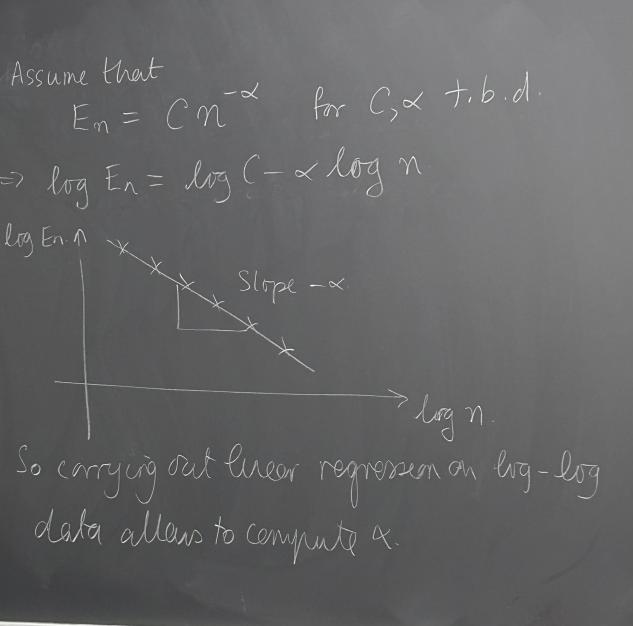
\includegraphics[width=0.5\linewidth]{Figures//lecture5/lec5-2.png}\]
Then, carrying out a linear regression on log-log data allows us to find the best $C$ and $\alpha$. 
\end{example}

\begin{example}
    Consider the integration $\int_0^1 t^{1/2} dt = \frac{2}{3}$.
    \begin{itemize}
        \item We use the Trapezoidal rule in this case and compare $\log E_n^{trap}$ vs $\log n$ again, but we find that $\alpha \approx 1.47$. THis is because the function is not so smooth. This has a reduced rate from $O(N^2)$ given by the theorem.\\
        \item We then compare $\log E_n^{simp}$ with $\log n$ using Simpson's rule, this gives that $\alpha \approx 1.499$. We did twice as much work but has no significant increase in convergence!
    \end{itemize}
\[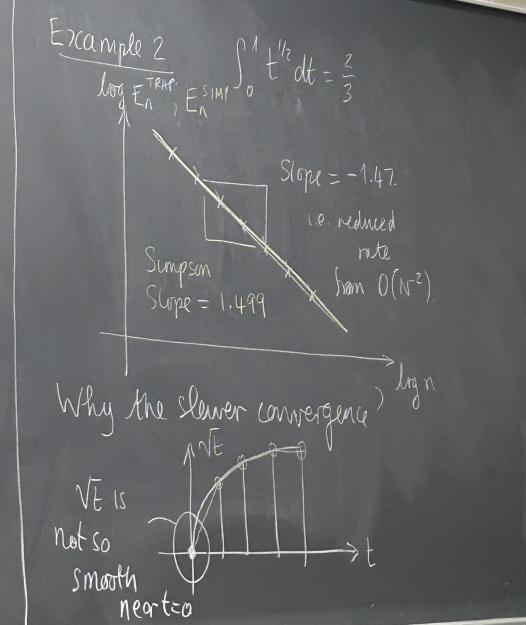
\includegraphics[width=0.5\linewidth]{Figures//lecture5/lec5-3.png}\]
    The point is that we have a loss of convergence because the function is $t^{1/2}$ not smooth at $t = 0$ as it has an infinite derivative there.
\end{example}

\begin{question}
    Can we explain this theoretically?
\end{question}

Indeed, let's consider $f(t) = t^\alpha$ with $0 < \alpha < 1$ and look at the error $t \in [0, h]$, we find that the error
\begin{align*}
    \int_0^h f(t) dt - \frac{h}{2} [f(0) + f(h)] &= \frac{h^{\alpha + 1}}{\alpha + 1} - \frac{h^{\alpha + 1}}{2}\\
    &= \frac{\alpha - 1}{\alpha + 1} h^{\alpha + 1}\\
    &= \frac{\alpha - 1}{\alpha + 1} N^{-(1+\alpha)} \tag*{Recall $h = 1/N$}
\end{align*}
Hence, we expect a rate of convergence at best $O(N^{-(1 + \alpha)}) = O(h^{1 + \alpha})$. Note that if $\alpha$ gets arbitrarily closer to $-1$, the convergence just completely fails. Here's an idea to adjust this:

\begin{idea}
    Why don't we use a smaller value of $h$ on the first interval? (e.g. replace $h$ by $h_1 = t_1 - t_0$, to be determined). In this case, the error would be (from the first interval), following the same argument
    \[\frac{\alpha - 1}{\alpha + 1} h_1^{1 + \alpha}\]
    If we want the error to be $O(h^2)$ for the trapezoidal rule, we want to select $h$ such that
    \[\frac{\alpha - 1}{\alpha + 1} h_1^{1 + \alpha} = c n^{-3}\]
    We want $n^{-3}$ in this since it will be added up with the other terms to together contribute to a total $n^{-2}$. (The local error should be one degree less than the global error). Hence, we want to choose $h_1 \sim n^{-3/(1+\alpha)}$, this will give error $c n^{-3}$ from first interval.\\
    What about the second interval? Well doing the same argument as before, this is from $h$ to $2h$, and we will still get an $h^{\alpha + 1}$. All of the errors would come from the second interval. So we do the same for the second, and then the same for the third. But at each time the difference between $h_n  - h_{n-1}$ gets larger and larger.\\

    In principle, we are trying to make a mesh that adapts around the function given here. Let's try to use a mesh that is non-uniformly spaced and tailored to the function we are trying to approximate. 
\end{idea}

\subsection{Mesh Grading}

Let's introduce a mesh grading function $\Gamma: [a, b] \to [0, 1]$ and choose nodes $t_k$ such that
\[\Gamma(t_k) = \frac{k}{N}\]
This is a mapping from a non-uniformly spaced nodes to uniformly spaced nodes.

\begin{example}
    Consider for example the following plot
\[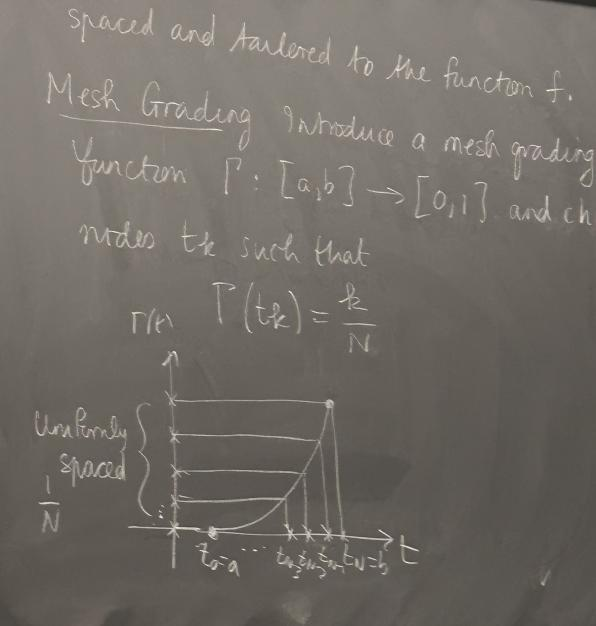
\includegraphics[width=0.5\linewidth]{Figures//lecture5/lec5-4.png}\]
    In this case, we have turned the non-uniform spaces to uniformly spaced nodes. 
\end{example}

To construct the function, we would want $\Gamma(a) = 0$ and $\Gamma(b) = 1$ with $t_0 = a$ and $t_N = b$. We also want that
\[C \geq \Gamma'(s) \geq c > 0\]
for all $s \in [a, b]$. We want to find an expression for error obtained by approximating 
\[\int_a^b f(t) dt \text{ by \underline{Composite Rule with nodes at $\{t_k\}$}}\]
In particular, we know it varies with $\Gamma$, so perhaps that makes the problem even more complicated.\\

Let's suppose that our base quadrature rule satisfies, by the Peano Kernel Theorem,
\[E_{[0, h]}(g) = \int_0^h g(t) ds - Q_{[0, h]}(g)  = \int_0^h K(s, h) g^{(p)}(s) ds\]
for some $p \in \Nbb$ and some kernel $K(s, h)$ depending on $s$ and $h$. 

\begin{example}
For example, if we are using the midpoint rule, then $p = 2$ and the kernel function $K_M$ for midpoint rule ($M$ denotes this is for the midpoint rule) is
\[K_M(s, h) = \begin{cases}
    1/2 s^2,\quad s < \frac{h}{2}\\
    1/2 (h - s)^2, s \geq \frac{h}{2}
\end{cases}\]
Notice that $K_M(s, h) = h^2 K_M(\frac{s}{h}, 1)$ is of $O(1)$.
\end{example}

In general, we will have that
\[K(s, h) = h^p K(\frac{s}{h}, 1) \sim h^p\]
Hence, the error
\begin{align*}
    E_{[0, h]}(g) &= h^p \int_0^h K(\frac{s}{h}, 1) g^{(p)}(s) ds\\
    &\leq h^p \max_{0 \leq s \leq h} |K(\frac{s}{h}, 1)| \int_0^h |g^{(p)}(s)| ds\\
    &\leq C h^p \int_0^h |g^{(p)}(s)| ds \tag*{Note that $C$ is independent of $g$}
\end{align*}

Now, we have that
\begin{align*}\allowdisplaybreaks
    E(\Gamma) &= \int_a^b f(t) dt - \sum_{k=0}^{N-1} Q_{[t_k, t_{k+1}]}(f)\\
    &= \sum_{k=0}^{N-1} \{\int_{t_k}^{t_{k+1}} f(t) dt - Q_{[t_k, t_{k+1}]}(f) \}\\
    &= \sum_{k = 0}^{N-1} E_{[t_k, t_{k+1}]}(f)\\
    &\leq C \sum_{k = 0}^{N-1} h^p_k \int_{t_k}^{t_{k+1}} |f^{(p)}(s)| ds \tag*{where $h_k = t_{k+1} - t_k$ and use inequality before}
\end{align*}
Note that $\frac{1}{N} = \Gamma(t_{k+1}) - \Gamma(t_k) = h_k \Gamma'(\xi_k)$ for some $\gamma_k \in (t_k, t_{k+1})$ with Mean Value Theorem. Hence, we have that
\[h_k = \frac{1}{N \Gamma'(\xi_k)}\]
This tends to $0$ as $N \to \infty$ (since we assumed that derivatives are bounded away from zero). Therefore, since $\Gamma$ is continuous, we have that

\[\xi_k \in (t_k,t_{k+1}) \text{ and } \Gamma'(\xi_k) \sim \Gamma'(s), s \in (t_k, t_{k+1})\]

Hence, we see that the expression
\[h_k^p \int_{t_k}^{t_{k+1}} |g^{(p)}(s)| ds = \int_{t_k}^{t_{k+1}} h_k^p |f^{(p)}(s)| ds \]
\[\approx \int_{t_k}^{t_{k+1}} \frac{1}{(N \Gamma'(s))^p} |f^{(p)}(s)| ds\]

As a consequence, we get that
\[E(\Gamma) \leq C N^{-p} \sum_{k = 0}^{N-1} \int_{t_k}^{t_{k+1}} \frac{|f^{(p)}(s)| ds}{\Gamma'(s)^p} = C N^{-p} \int_a^b \frac{|f^{(p)}(s)|}{\Gamma'(s)^p} ds  \]

\textcolor{red}{Thus, we have obtained a magical formula: Given a mesh grading function, we can express the error in terms of the Mesh Grading Function!}\\

Our task now is to find an appropriate Mesh Grading function $\Gamma$ that minimizes this error $E(\Gamma)$. Let's denote the optimal by $\Gamma_*$ (assume it exists and is unique), and consider what properties it must satisfy?\\

Indeed, consider
\[\Gamma(s) = \Gamma_*(s) + \epsilon \eta(s) \quad \epsilon << 1 \text{ and } \eta(a) = \eta(b) = 0\]
This fixes the endpoints and still keeps the grading. For a stationary point of $E(\Gamma)$, we fix $\eta$ and vary $\epsilon$ and consider trying to solve
\begin{align*}
    \frac{d}{d\epsilon} E(\Gamma_* + \epsilon \eta) |_{\epsilon = 0} &= 0
\end{align*}
Computing the LHS gives
\begin{align*}
    0 &= C N^{-p} \int_a^b ds \frac{|f^{(p)}(s)| \eta'(s)}{\Gamma'_*(s)^{p+1}} \tag*{Quotient Rule with respect to $\epsilon$}
\end{align*}
But this is $0$ for all choices of $\eta$ such that $\eta(a) = \eta(b) = 0$. Note that if we take the second derivative, we furthermore have
\[C N^{-p} p (p +1) \int_a^b ds |f^{(p)}(s)| \frac{\eta'(s)^2}{\Gamma'_*(s)^{p+2}} \geq 0\]
By the second derivative test, we know that $\epsilon = 0$ is a minimum so $E(\Gamma_*)$ is minimal.\\

We integrate by parts on the $0 = \int_a^b ds \frac{|f^{(p)}(s)| \eta'(s)}{\Gamma'_*(s)^{p+1}}$ to get 
\begin{align*}
    0 &= [\frac{|f^{(p)}(s)|}{\Gamma'_*(s)^{p+1}} \eta(s)]_a^b - \int_a^b \eta(s) \frac{d}{ds} \frac{|f^{(p)}(s)|}{\Gamma'_*(s)^{p+1}}\\
    &= 0 - \int_a^b \eta(s) \frac{d}{ds} \frac{|f^{(p)}(s)|}{\Gamma'_*(s)^{p+1}} \tag*{Since $\eta(a) = \eta(b) = 0$}
\end{align*}
This is the integral of a non-negative function, so we get that
\[\frac{d}{ds} \frac{|f^{(p)}(s)|}{\Gamma'_*(s)^{p+1}} = 0, a < s < b\]
Hence, we have that
\[\Gamma'_*(s)^{p+1} \alpha |f^{(p)}(s)|\]
with some constant, and $\Gamma_*(a) = 0$ and $\Gamma_*(b) = 1$.\\

Now we claim that the optimal function is
\[\Gamma_*(t) = \frac{\int_a^t |f^{(p)}(s)|^{1/(p+1)} ds}{\int_a^b |f^{(p)}(s)|^{1/(p+1)} ds}\]
We can check that it satisfies:
\begin{enumerate}
    \item $\Gamma_*(a) = 0$ and $\Gamma_*(b) = 1$
    \item $\frac{d}{ds} \frac{|f^{(p)}(s)|}{\Gamma'_*(s)^{p+1}} = 0, a < s < b$
\end{enumerate}

Let $m(f)$ be the denominator, then we can write
\[\Gamma_*(t) = \frac{1}{m(f)} \int_a^t |f^{(p)}(s)|^{1/(p+1)} ds, a \leq t \leq b\]

\begin{question}
    What is the Error we get for the optimal mesh?
\end{question}

Substituting this into $E$, we have that
\[E(\Gamma_*) \leq C N^{-p} m^p \int_a^b |f^{(p)}(s)|^{1 - \frac{p}{1+p}} ds\]

Note that $1 - \frac{p}{p+1} = \frac{1}{p+1}$. Simplifying this, we have that
\[E(\Gamma_*) \leq C N^{-p} m^p \int_a^b |f^{(p)}(s)|^{1/(p+1)} ds = C N^{-p} m(f)^{p+1}\]

Putting it together, we summarize this into a theorem.
\begin{theorem}
    Suppose $f$ satisfies
    \[m(f) = \int_a^b |f^{(p)}(s)|^{1/(p+1)} ds < \infty\]
    where $f^{(p)}$ is not identically zero (if it is there's nothing to prove). Let $Q_{[0, h]}$ be a quadrature rule that is exact for all polynonmials $r \in \Pbb_p$. Then there exists a mesh grading function $\Gamma_*$ such that
    \[E(\Gamma_*) \leq C N^{-p} m(f)^{p+1} = C N^{-p} ||f^{(p+1)}||_{L^{1/p}}\]
    where $C$ is independent of $f$.
\end{theorem}

\begin{remark}
    This is a very fundamental theorem in numerical analysis, but you don't really find them in textbooks these days. One good source is from DeVore and Lorentz.
\end{remark}

\begin{example}
    Let's try $f(t) = t^\alpha$ with $-1 < \alpha < 1$ and choose the Trapezoidal rule, so $p = 2$. Then we note that
    \[f^{(p)}(t) \sim t^{\alpha - p}\]
    Then we see that for $s \geq 0$
    \[\int_0^s |f^{(p)}(t)|^{1/(p+1)} dt = \int_0^s t^{\frac{\alpha - p}{p+1}} dt = \int_0^s t^{\frac{\alpha - 2}{3}} = s^{(a+1)/3} < \infty \]
    Thus $m(f) < \infty$. The Theorem then implies that Trapezoidal Rule gives rates $\mathcal{O}(N^{-2})$ now and we choose
    \[\Gamma_*(t_k) = \frac{k}{N} \text{ and } \Gamma_*(s) = s^{(\alpha + 1)/3}\]
    Hence,
    \[t_k^{(a + 1)/3} = \Gamma_*(t_k) = \frac{k}{N} \iff t_k = (\frac{k}{N})^{3/(1 + \alpha)}, k = 0, 1, ..., N\]
    \mattie{Note that $a$ and $\alpha$ are used interchangeably in this example. Constants are also ignored in this examole.}
\end{example}

\newpage
\section{Lecture 6}

The story so far ...

\mattie{TODO: fill in later, just review of last lecture}

We found that an optimal solution exists with
\[\Gamma_\star(a) = 0; \Gamma_\star(b) = 1\]
satisfying the differential equation
\[\frac{d}{ds} \frac{|f^{(p)}(s)|}{\Gamma_\star'(s)^{p+1}} = 0, s \in [a, b]\]
where $p$ is related to the order of the basic quadrature rule $Q$. The results in
\[ | E[f, \Gamma_\star] | \leq C N^{-p} m_p(f)^{p+1}\]
where $m_p(f)$ is the integral
\[m_p(f) = \int_a^b |f^{(p)}(s)|^{1/(p+1)} ds\]

We ended up with the theorem:
\begin{theorem}
    Suppose $f$ satisfies
    \[m(f) = \int_a^b |f^{(p)}(s)|^{1/(p+1)} ds < \infty\]
    where $f^{(p)}$ is not identically zero (if it is there's nothing to prove). Let $Q_{[0, h]}$ be a quadrature rule that is exact for all polynonmials $r \in \Pbb_p$. Then there exists a mesh grading function $\Gamma_*$ such that
    \[E(\Gamma_*) \leq C N^{-p} m(f)^{p+1} = C N^{-p} ||f^{(p+1)}||_{L^{1/p}}\]
    where $C$ is independent of $f$.
\end{theorem}

In some sense, this is the most fundamental result in numerical analysis because it tells you how to maximal approximate a function given a constrant on the number of points you can use.

\subsection{Approximating Optimal Grid}

\begin{question}
    What are the bad news?
\end{question}

Here are some drawbacks on this theorem:
\begin{itemize}
    \item Often times, we cannot evaluate $\Gamma_\star$ in closed form. Often times, we only know that
    \[\Gamma_\star(s) = \frac{1}{\int_a^b |f^{(p)}(s)|^{1/(p+1)} ds} \int_a^s |f^{(p)}(s)|^{1/(p+1)} ds \]
    \item Even if we can, we might not be able to write down an explicit inverse.
\end{itemize}

\begin{question}
    Let's suppose that we replace $\Gamma_\star(s)$ by an approximation $\Tilde{\Gamma}$ (where $\Tilde{\Gamma}$ is some mesh-grading function). Do we still get the same advantages as if we used $\Gamma_\star$?
\end{question}

Let's suppose $\Tilde{\Gamma} = \Gamma_\star + \epsilon \eta$ where $+\epsilon \eta$ is some perturbation where $\eta(a) = \eta(b) = 0$ and $\epsilon << 1$. Let the associated nodes be $\{\Tilde{t}_k\} = \Tilde{P}$ where
\[\Tilde{\Gamma}(\Tilde{t}_k) = \frac{k}{N}, k = 0, 1, ..., N\]
Can we expect $\Tilde{t}_k \to t_k$ as $\epsilon \to 0$?\\

To do this, we need to estimate
\begin{align*}
    0 &= \frac{k}{N} - \frac{k}{N}\\
    &= \Tilde{\Gamma}(\Tilde{t}_k) - \Gamma_\star(t_k)\\
    \iff 0 &= \Tilde{\Gamma}(\Tilde{t}_k) - \Tilde{\Gamma}(t_k) + \epsilon \eta(t_k)\\
    \iff -\epsilon \eta(t_k) &\approx (\Tilde{t}_k - t_k) \Tilde{\Gamma}'(t_k) \tag*{Mean Value Theorem}\\
    &= (\Tilde{t}_k - t_k) (\Gamma'_\star(t_k) + \epsilon \eta(t_k))
\end{align*}
Hence, we have that
\[t_k - \Tilde{t}_k \approx \frac{\epsilon \eta(t_k)}{\Gamma'_\star(t_k) + \epsilon \eta(t_k)} = O(\epsilon).\]

\begin{question}
    How does the error $E(f; \Tilde{\Gamma})$ compare with $E(f; \Gamma_\star)$? Notice that $E[f; \Tilde{\Gamma}] = E[f; \Gamma_\star + \epsilon \eta] \to E[f, \Gamma_\star]$ as $\epsilon \to 0$. Can we be more precise here? 
\end{question}

Last week, we proved that (as $\Gamma_\star$ is optimal),  
\[\frac{d}{d\epsilon} E(\Gamma_\star + \epsilon \eta) |_{\epsilon = 0} = 0\]
for all $\eta$ such that $\eta(a) = \eta(b) = 0$. We also showed that
\begin{align*}
    \frac{d^2}{d\epsilon^2} E(\Gamma_\star + \epsilon \eta) |_{\epsilon = 0} &= C N^{-p} p(p+1) \int_a^b ds \frac{|f^{(p}(s)|}{\Gamma'_\star(s)^{p+2}} \eta'(s)^2\\
    &= C N^{-p} p (p+1) m^{p+1}(f) \int_a^b ds \frac{\eta'(s)^2}{\Gamma'_\star(s)}  \tag*{Since $\Gamma'_\star(s) = m^{-1} |f(s)|^{1/(p+1)}$ in summary}
\end{align*}
Let's call
\[D(\Gamma_\star, \eta) \coloneqq \frac{d^2}{d\epsilon^2} E(\Gamma_\star + \epsilon \eta) |_{\epsilon = 0} \]


What we have done is the following theorem:
\begin{theorem}
    Suppose we have an optimal mesh grading function perturbed in a way such that
    \[\Gamma_\star \to \Gamma_\star + \epsilon \eta, \eta(a) = \eta(b) = 0\]
    Then we have the following approximation of $\Gamma_\star$:
    \begin{enumerate}
        \item Optimal nodes: $t_k \to \Tilde{t}_k + O(\epsilon)$.
        \item $E(f; \Gamma_*) \to E(f, \Gamma_*) + \frac{1}{2} \epsilon^2 D(\Gamma_*, \eta)$
    \end{enumerate}
\end{theorem}

\begin{remark}
    This is great news! This means that $E(f; \Gamma_*)$ is very insensitive to the change of notes. If $\Tilde{t}_k - t_k = O(\epsilon)$, then $E(f; \Tilde{\Gamma}) - E(f; \Gamma) = O(\epsilon^2)$. This means that a $10\%$ error in the approximation of the mesh grading gives a $1\%$ difference in the error functional. 
\end{remark}

But there's more bad news ... we don't know what the $t_k$'s are to begin with, so how can we approximate them?

\begin{question}
    What characterizes an optimal grid?
\end{question}

Recall that optimal grid function satisfies
\[\frac{d}{ds} \frac{|f^{(p)}(s)|}{\Gamma'_\star(s)^{p+1}} = 0, s \in [a, b] \quad (\dagger)\]
We could try to solve for this differential equation, and recall as from last week, $\Gamma'_\star(s)$ came from
\[\Gamma'_\star(s) \simeq \frac{1}{N h_k}, s \in (t_k, t_{k+1})\]
We can use this to rewrite the differential equation as
\[\frac{d}{ds} \frac{|f^{(p)}(s)|}{\Gamma'_\star(s)^{p+1}} \simeq N^{(p+1)} h_k^{p+1} |f^{(p)}(s)|, s \in (t_k, t_{k+1})\]
\[\simeq N^{(p+1)} h_k^p \int_{t_k}^{t_{k+1}} |f^{(p)}(t)| dt\]
\[\simeq N^{(p+1)} C | E_{[t_k, t_{k+1}]}(f)|, s \in (t_k, t_{k+1}) \]
where $| E_{[t_k, t_{k+1}]}(f)|$ is the \underline{local error} in approximating $\int_{t_k}^{t_{k+1}} f(t) dt$. Hence, $(\dagger)$ means that the local errors $|E_{[t_k, t_{k+1}]}(f)|$ for $k = 0, 1, ..., N-1$ are roughly equal on an optimal grid.

\begin{question}
    Let's suppose we have a grid where the error on a particular integral is much larger than the others. This is nowhere near close to the optimal grid (since its errors are roughly the same on all intervals). How can we reduce the error on this particular interval?
\end{question}

Recall that 
\[|E_{[t_k, t_{k+1}]}(f)| \simeq h_k^{p+1} |f^{(p)}(s)|, s \in (t_k, t_{k+1})\]
We can't change $|f^{(p)}(s)|$, so we want to try to \textbf{reduce $h_k$}, then this will reduce $|E_{[t_k, t_{k+1}](f)}|$.\\

We could get smaller error by adding new points in the interval $(t_k, t_{k+1})$. Why don't we add in a new point between $(t_k, t_{k+1})$? We will subdivide the interval $(t_k, t_{k+1})$ by putting it in as the midpoint.
\[ 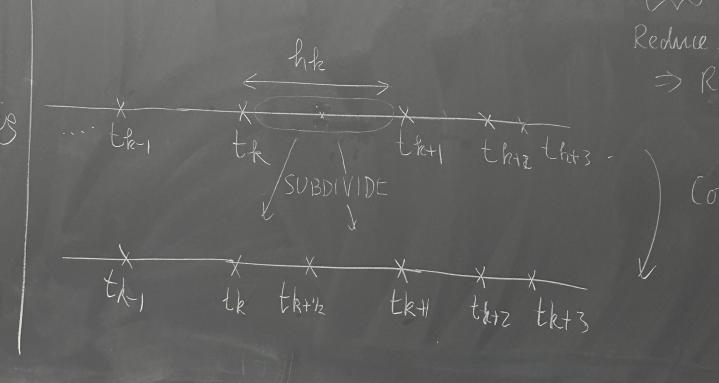
\includegraphics[width=0.6\linewidth]{Figures//lecture6/lec6-1.png}\]
This corresponds to creating a new partition $P_{new}$ by removing $(t_k, t_{k+1})$ from $P$ and adding $(t_k, t_{k+1/2})$ and $(t_{k+1/2}, t_{k+1})$.\\

In general, we could create an inductive algorithm as follows:
\[    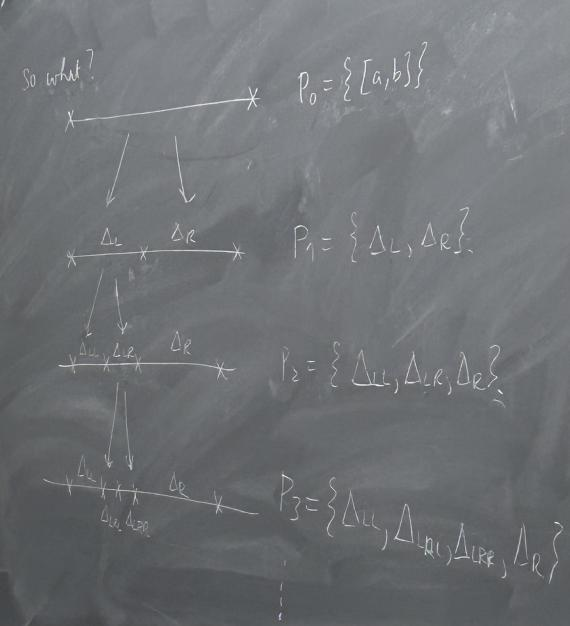
\includegraphics[width=0.5\linewidth]{Figures//lecture6/lec6-2.png}\]
We start with the entire interval, then we subdivide once. We look at the interval with the highest error, we subdivide that, and then we keep doing this to generate a non-uniform grid.\\

In general, we have a sequence of partitions $P = \{\Delta\}_{\Delta \in P}$ such that
\begin{itemize}
    \item $\Delta$ are non-overlapping.
    \item $\bigcup_{\Delta \in P} \Delta = [a, b]$.
\end{itemize}

This seems to be a promising algorithm! But, in order to be able to run the algorithm, we still need two things:
\begin{enumerate}
    \item A basic quadrature rule $\int_\Delta f(t) dt \simeq Q(\Delta)$.
    \item A criterion / way of estimating the error
    \[\epsilon(\Delta) \simeq |\int_\Delta f(t) dt - Q(\Delta) |\]
\end{enumerate}

Let's suppose we have $Q(\Delta)$ and $\epsilon(\Delta)$, here's the algorithm

\begin{tcolorbox}[standard jigsaw,opacityback=0]\\
\begin{algorithm}[H]
\caption{Subdivide Approximations - SUBDIVIDE(P)}
\KwData{$Q(\Delta)$ and $\epsilon(\Delta)$ on interval $[a, b]$}
\KwResult{A partition on $[a, b]$ approximating the optimal grid}
We initialize the algorithm by setting $P = \{[a, b]\}$ and calling $\operatorname{SUBDIVIDE}(P)$.\;
1. Find $\Delta_m \in P$ such that $\epsilon(\Delta_m) = \max_{\Delta \in P} \epsilon(\Delta)$\;
2. Split $\Delta_m \to \Delta_L, \Delta_R$ where we break at the midpoint\;
3. Let $\Tilde{P} = (P \setminus \Delta_m) \cup \{\Delta_L, \Delta_R\}$\;
4. If $\sum_{\Delta \in \Tilde{P}} \epsilon(\Delta) \leq TOL * \sum_{\Delta \in P} |Q(\Delta)|$ (TOL is some tolerance constant), then return $\sum_{\Delta \in \Tilde{P}} Q(\Delta)$\; Else, we call $\operatorname{SUBDIVIDE}(\Tilde{P})$;
\end{algorithm}
\end{tcolorbox}

This is a great algorithm in theory, but, in practice, we want to
\begin{itemize}
    \item Put a $\operatorname{max\_iter}$ on the lengths of recursion.
    \item Rather than refining one interval, we refine all intervals $\Delta$ whose $\epsilon(\Delta) \geq 90\% \cdot \max_{\Delta \in P} \epsilon(\Delta)$. 
\end{itemize}

\begin{question}
    We still need a pair $Q(\Delta)$ and $\epsilon(\Delta)$! How can we be get a pair?
\end{question}

\begin{example}
    Let's take $Q(\Delta)$ to be the trapezoidal rule, meaning that
    \[Q_{[0, h]}(f) = \frac{h}{2} [f(0) + f(h)]\]
    How to approximate this? Well, can we use Simpson's Rule to compute a more accurate approximation and take the difference? Indeed, let's consider the difference between Simpson's Rule and Trapezoidal Rule
    \[\epsilon(\Delta) = |\frac{h}{6} \{f(0) + 4 f(h/2) + f(h)\} - \frac{h}{2} \{f(0) + f(h)\}|\]
    In this case, we obtain that
    \begin{align*}
        \epsilon(\Delta) &= \frac{h}{6} |-2f(0) + 4 f(\frac{h}{2}) - 2 f(h)|\\
        &= \frac{h}{3} |-f(0) + 2 f(\frac{h}{2}) - f(h)|, \tag*{We have $\Delta = (0, h)$}
    \end{align*}
\end{example}

The instructor begins to perform a live demo of the algorithm described in this example.

% About 20 runs, 2.061

The proposed algorithm above eventually failed on $f(t) = 1/\sqrt{t}$ because it's not smooth at the origin.

\begin{example}
    Let's instead consider $Q(\Delta)$ to be the midpoint rule and write
    \[Q_{[0,h]}(\Delta) = h f(\frac{h}{2})\]
    This will allow us to integrate $f(t) = 1/\sqrt{t}$. However, if we take $\epsilon(\Delta)$ to be Simpson's Rule, we will still fail - we are still going to evaluate $f(0)$. Why don't we try to use the midpoint to error?\\

    We know that $E_M = I - Q_M(h) = C h^3 $ (we proved this), then consider a composite midpoint rule defined by:
    \[E_M^c= I - Q_M^L(\frac{h}{2}) - Q_M^R(\frac{h}{2}) = (I^L - Q_M^L) + (I^R - Q_M^R) = C(\frac{h}{2})^3 + C(\frac{h}{2})^3 = \frac{1}{4} C h^3\]

    Hence we have that
    \[\begin{cases}
        I - Q_M(h) = C h^3,\\
        I - Q_M^c(\frac{h}{2}) = \frac{1}{4} C h^3
    \end{cases}\]
    Solving this two lineat equations with unknowns $I$ and $C$, we have that
    \[I = \frac{1}{3} (4 Q_M^c(h/2) - Q_M(h))\]
    Thus, we should take $\epsilon(\Delta)$ to
    \begin{align*}
        \epsilon(\Delta) &= |\frac{1}{3} (4 Q_M^c(h/2) - Q_M(h)) - Q_M|\\
        &= \frac{4}{3} |Q_M^c - Q_M|\\
        &= \frac{4}{3} |\frac{h}{2} [f(h/4) + f(3h/4)] - h f(h/2)|\\
        &= \frac{2h}{3} |f(h/4) - 2 f(h/2) + f(3h/4)|
    \end{align*}
    This is called \textbf{Richardson's Rule}. In general, you could do a similar Richardson extraction for any quadrature rule.
\end{example}

\newpage
\section{Lecture 7}

\subsection{Euler's Method}

Let's consider the IVP
\[\frac{du}{dt}(t) = f(t, u(t)), t \in [a, b]\]
with the initial condition $u(a) = u_0$ where $f: [a, b] \times \Rbb^d \to \Rbb^d$ is continuous and Lipschitz in the second argument. In other words, we recall that there exists $L \geq 0$ such that
\[|f(t, u) - f(t, v)| \leq L |u - v|, \forall u, v \in \Rbb^d.\]
Thus, we are in the setting to aplly Picard's Theorem, and we have a unique solution satisfying the IVP.

\begin{question}
    How do we approximate the solution?
\end{question}
For far, we have been looking at a simpler setting where $f$ is not dependent of $u$ - this is why we had the whole discussion abotu quadratures in this class. Let's recall the proof of \textbf{Picard's Theorem} - it suggests that we write the problem in the form
\[u(t) = u_0 + \int_a^t f(s, u(s)) ds, t \in [a, b]\quad (\star)\]
This is easier for us to do for theory, so we will try to see how far we can get away with this.\\

Let's introduction a partition in time $t$ into
\[a = t_0 < t_1 < t_2 < .... < t_n = b\]
We seek vectors $u_0, ..., u_n \in \Rbb^d$ such that 
\[u(t_n) \simeq u_n\quad (\text{in some sense})\]

Let's choose $t = t_1$ in $(\star)$, then we have that, by the proof of Picard's Theorem,
\[u(t_1) = u_0 + \int_a^{t_1} f(s, u(s)) ds\]
But the integral is generally difficult to integrate since we don't know what $u(s)$ is! Our previous work suggests that we approximate the integral using an appropriate rule.\\

Let's say we want to use the trapezoidal rule, but we immediately run into problems! We don't know what $u(t_1)$ is! We only know that $u(a) = u_0$, so $f(a, u(a)) = f(a, u_0)$. Therefore, let's just use the Left-Hand Endpoint rule to approximate the integral - recall that
\[\int_0^h g(s) ds \approx h g(0)\]
By the Peano Kernel theorem, we know that
\[\int_0^h g(s) ds = h g(0) + \frac{1}{2} h^2 g'(\xi), \text{ for some } \xi \in (0, h)\]
Our scheme them becomes 
\[u(t_1) \simeq u_1 = u_0 + (t_1 - t_0) f(t_0, u_0) \]

In general, we get - for a given $u_0$,
\[u_{n+1} = u_n + (t_{n+1} - t_n) f(t_n, u_n), n = 0, 1, ...., N-1\]
Roughly speaking, we are given $(t_0, u_0)$ and we only look at the direction at $t_0$ to tell us where to go. Once you get to $t_1$, we look at the direction given by the gradient at the current location, rather than the true location.
\[ 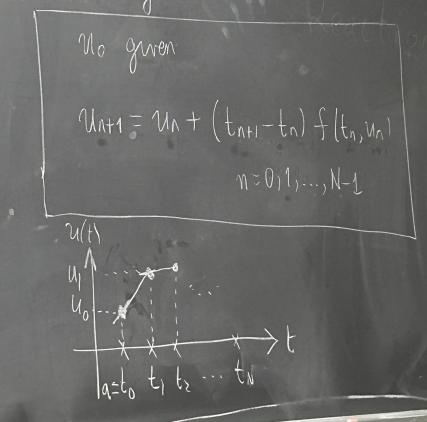
\includegraphics[width=0.5\linewidth]{Figures/lecture7/lec7-1.png}\]
This method is called \textbf{Euler's method}. This computes a set of values $\{u_n\}_{n=0}^N$ such that $u_n \simeq u(t_n)$.

\begin{question}
    Thus, this leads us to ask
    \begin{itemize}
        \item Does the scheme converge? In other words, can we show that
        \[\max_{0 \leq n \leq N} |u_n - u(t_n)| \to 0 \text{ as } N \to \infty \text{ and / or } |t_{n+1} - t_n| \to 0\]
        \item  If so, then at what rate does the convergence occur?
    \end{itemize}
\end{question}

Let's consider a sequence of uniform partitions where $t_n = a +  n h$ where $n = 0, 1, ..., N$ and $h = \frac{(b-a)}{N}$. Consider the error at time $t_{n+1}$, which is $u(t_{n+1}) - u_{n+1}$.
\begin{align*}
    u(t_{n+1}) - u_{n+1} &= u(t_n) + \int_{t_n}^{t_{n+1}} f(s, u(s)) ds - u_n - h f(t_n u_n)\\
    &= ( u(t_n) - u_n ) + \int_{t_n}^{t_{n+1}} f(s, u(s)) ds - h f(t_n, u_n)
\end{align*}
But the term $\int_{t_n}^{t_{n+1}} f(s, u(s)) ds - h f(t_n, u_n)$ is not really an approximation. If we apply the left hand rule on $\int_{t_n}^{t_{n+1}} f(s, u(s)) ds$, we should be getting $h f(t_n, u(t_n))$ rather than $h f(t_n, u_n)$. This isn't just quadrature error, it's a fundamental gap in approximation.\\

We will instead rewrite the second term a sum of two terms:
\[[\int_{t_n}^{t_{n+1}} f(s, u(s)) ds - h f(t_n, u(t_n))] + [h f(t_n, u(t_n)) - h f(t_n, u_n)] \]

Now the term $\int_{t_n}^{t_{n+1}} f(s, u(s)) ds - h f(t_n, u(t_n))$ is a quadrature error! Let's consider each term as once\allowdisplaybreaks
\begin{align*}
    \int_{t_n}^{t_{n+1}} f(s, u(s)) ds - h f(t_n, u(t_n)) &= \int_{t_n}^{t_{n+1}} \frac{du}{ds}(s) ds - h \frac{du}{dt}(u_n) \tag*{Since $du/dt = f(t, u(t))$}\\
    &= \frac{1}{2} h^2 \frac{d^2 u}{d t^2}(\xi_n) \tag*{Using the Remainder rule for LHR, for some $\xi_n \in (a, b)$}
\end{align*}
For the other term, we have
\begin{align*}
    h |f(t_n, u(t_n)) - f(t_n, u_n))| &\leq h L |u(t_n) - u_n| \tag*{Lipschitz Condition}
\end{align*}

Combining the two inequality / estimate, we have that
\begin{align*}
    |u(t_{n+1}) - u_{n+1}| &\leq (1 + hL) |u(t_n) - u_n| + \frac{1}{2} h^2 M_2 \tag*{where $M_2 = \max_{a \leq t \leq b} |\frac{d^2 u}{d t^2}(t)|$}
\end{align*}
This holds for all $n = 0, 1, ..., N-1$.\\

Let $e_n = |u(t_n) - u_n|$, then we know that $e_0 = 0$ and $e_1 \leq \frac{1}{2} h^2 M_2$. Going down the list
\begin{itemize}
    \item $e_2 \leq (1 + hL) e_1 + \frac{1}{2} h^2 M_2$
    \item $e_3 \leq (1 + hL) e_2 + \frac{1}{2} h^2 M_2$
\end{itemize}
The bound is getting bigger and bigger for higher $n$ and $e_n$. This does not seem promising. Now, we could bound this somewhat with
\[e_2 \leq (1 + hL) e_1 + \frac{1}{2} h^2 M_2 \leq \frac{1}{2} h^2 M_2 \{1 + (1 + hL)\}\]
\[e_3 \leq \frac{1}{2} h^2 M_2 \{1 + (1 + hL) + (1 + hL)^2\}\]
In general we have that
\[e_n \leq ... \leq \frac{1}{2} h^2 M_2 \sum_{j = 0}^{n-1} (1 + h L)^j, n = 1, 2, ..., N \]

Computing this finite geometric sum, we have that
\[e_n \leq \frac{1}{2} h^2 M_2 \frac{(1 + hL)^n - 1}{hL} \]

Note that $1 + r \leq e^r$ for all $r$, so $(1 + r)^n \leq e^{nr}$, so we have
\[e_n \leq \frac{M_2 h}{2L} \{e^{n hL} - 1\}\]

Now, $nh = t_n - t_0$, so
\[e^{nhL} = e^{L(t_n - a)}\]
Hence we have that
\begin{align*}
    e_n &\leq \frac{h M_2}{2L} \{e^{L(t_n - a) - 1\}
\end{align*}
for $n = 0, 1, ..., N$. Thus, we have proven the following theorem:

\begin{theorem}
    Let $\{u_n\}$ be the output from Euler. If $u \in C^2[a, b]$, then
    \[\max_{0 \leq n \leq N} |u(t_n) - u_n)| \leq \frac{h M_2}{2L} (e^{L(b-a)} - 1) \]
    where $L$ is the Lipschitz constant for $f$ and $M_2 = \max_{a \leq t \leq b} |u''(t)|$.
\end{theorem}

\begin{remark}
    We have that
    \begin{enumerate}
        \item The Theorem shows that the method is convergent. So
        \[\lim_{N \to \infty} |u(t_n) - u_n| = 0, \forall n\]
        and that the rate is $O(h) = O(N^{-1})$.
        \item Suppose that $f(t, u) = \lambda u$, $a = 0$, and $b = T$, and $u(a) = u(0) = 1$. Hence we are solving that $u' = \lambda u$ with $u(0) = 1$, so $u(t) = e^{\lambda t}$. The Euler method reads as follows
        \[u_{n+1} = u_n + h f(t_n, u_n) = u+n + \lambda h u_n = (1 + \lambda h) u_n\]
        Hence, in general, Euler's method gives.
        \[u_n = (1 + \lambda h)^n, n = 0, 1, ..., N\]On the other hand, $u(t_n) = e^{\lambda n h}$.  Recall that $h = \frac{T}{n}$, and note that
        \[u_n = (1 + \frac{\lambda T}{N})^N \to e^{\lambda T} \text{ as $N \to \infty$}\]
        \item Continuing the example, we find the Lipschitz constant $L = |\lambda|$ because
        \[|f(t, u) - f(t, v)| = |\lambda u - \lambda v| = |\lambda| |u- v|\]
        The true solution is $u(t) = e^{\lambda t}$, so
        \[M_2 = \max_{0 \leq t \leq T} |u''(t)| = \max_{0 \leq t \leq T} |\lambda^2 e^{\lambda t}| \leq |\lambda^2| \max(1, e^{\lambda T})\]
        Our error bound is therefore
        \[h |\lambda|^2 \frac{1}{2 |\lambda|} \max(1, e^{\lambda T}) (e^{|\lambda| T} - 1)  \]
        \[= \frac{h}{2} |\lambda|  \max(1, e^{\lambda T}) (e^{|\lambda| T} - 1)  \]
        In comparision, the true error is
        \[u(t_N) - u_N = e^{\lambda T} - (1 + \frac{\lambda T}{N})^N \geq 0\]
        \item How tight is the bound? The following estimate will be helpful.
\begin{lemma}
    Let $\lambda \in \Rbb$ and $N \in \Nbb$. If $\frac{|\lambda| T}{N} < 1$, then we have
    \[Q \coloneqq e^{-\lambda T} (1 + \frac{\lambda T}{N})^N \leq 1 - \frac{\lambda^2 T^2}{2N} + \frac{\lambda^3 T^3}{3N^2}\]
\end{lemma}

\begin{proof}
    Suppose that $|\lambda| T < N$, then taking the natural log of $Q$ gives
    \[\ln Q = - \lambda T + N \ln(1 + \frac{\lambda T}{N})\]
    Doing the Taylor expansion, we have that
    \[\ln Q = - \lambda T + N (\frac{\lambda T}{N} - \frac{1}{2} (\frac{\lambda T}{N})^2 + \frac{1}{3} (\frac{\lambda T}{N})^3 - ...)\]
    \[\leq -\lambda T + N \{\frac{\lambda T}{N} - \frac{\lambda^2 T^2}{2N^2} - \frac{\lambda^3 T^3}{3 N^3}\}\]
    This inequality is obvious when $\lambda < 0$ because the neglected terms are all negative. If $\lambda > 0$, $[-\frac{1}{2n} (\frac{\lambda T}{N})^{2n} + \frac{1}{2n+1} (\frac{\lambda T}{N})^{2n+1}]$are all negative whose modulous decreases monotonically.\\

    Hence, we conclude that
    \[\ln Q \leq -\frac{\lambda^2 T^2}{2N} + \frac{\lambda^3 T^3}{3N^2} < 0\]
    Now taking an exponential on both sides and recalling that $e^{r} \leq 1 + r$ for $r < 0$, so we have
    \[Q \leq 1 - \frac{\lambda^2 T^2}{2N} + \frac{\lambda^3 T^3}{3N^2}\]
    \mattie{to be corrected by the instructor}
\end{proof}
Using the Lemma, we get that $u(t_n) - u_n = e^{\lambda T} (1 - Q) \geq e^{\lambda T} [\frac{\lambda^2 T^2}{2N} - \frac{\lambda^3 T^3}{3N^2}]$, which is approximately $e^{\lambda T} \frac{\lambda^2 T^2}{2N}$ when $\frac{|\lambda| T}{N} << 1$.\\

We then consider two cases:
\begin{itemize}
    \item If $0 < \lambda T << 1$, the error bound in this case $(h = 1/N)$ is $\frac{\lambda T e^{\lambda T}}{2N} (e^{\lambda T} - 1) \simeq \frac{\lambda T}{2N} \lambda T = \frac{\lambda^2 T^2}{2N}$, so our bound is very tight in this case! This shows that our bound is sharp in this case.
    \item If $\lambda < 0$, the error bound reads 
    \[\frac{|\lambda| T}{N} (e^{|\lambda| T} - 1)\]
    whereas the true error is
    \[u(t_N) - u_N \simeq e^{\lambda T} \frac{\lambda^2 T^2}{2N}\]
    Since $\lambda$ is negative, the true bound is tight, but the bound given by the Theorem explodes by a factor of $e^{|\lambda| T}  \frac{e^{|\lambda| T} - 1}{|\lambda T|} \sim \begin{cases}
        1, \quad |\lambda| T << 1\\
        \frac{e^{2|\lambda| T}}{|\lambda| T}, \text{ otherwise}
    \end{cases}$
\end{itemize}
Hence, we cannot use it to estimate the error quantitatively. The problem comes from the Lipschitz constant,where we lose information on the sign.
    \end{enumerate}
\end{remark}

Let's do an application. Recall Fisher's Equation is
\[\frac{\partial u}{\partial t} = \epsilon \Delta u + \lambda u(1 - u), \epsilon, \lambda > 0\]
Let's consider the 1D case so $\Delta u = \frac{\partial^2 u}{\partial x^2}$. Let's look for $2\pi$-periodic solutions in space, ie. of the form
\[u(x, t) = \sum_{k \in \Zbb} c_k(t) e^{i k x}\]
Note that $u(x + 2\pi ,t) = u(x, t)$ and $c_k(t)$ are functions of time.\\

Substitute into the PDE and equate Fourier coefficients, and we have
\[\frac{dc_k}{dt}(t) = - \epsilon k^2 c_k(t) + \lambda c_k(t) - \lambda  \frac{1}{2\pi} \int_{-\pi}^{+\pi} u(x, t)^2 e^{-i k x} dx \]

Now for the last term, we know that
\begin{align*}
    \frac{1}{2\pi} \int_{-\pi}^{+\pi} u(x, t)^2 e^{-i k x} dx &= \frac{1}{2\pi} \sum_{\ell, m} c_\ell c_m \int_{-\pi}^{\pi} e^{i(\ell +m -k)x} dx\\
    &= \sum_{\ell, m} c_\ell c_m \delta_{\ell + m, k} \tag*{Dirac Delta Function}\\
    &= \sum_\ell c_\ell c_{k-\ell}\\
    &= (c \star c)_k \tag*{Convolution}
\end{align*}
Hence, the $c_k$'s satisfy
\[\frac{dc_k}{dt}(t) = - \epsilon k^2 c_k + \lambda c_k - \lambda (c \star c)_k\]
This is an infinite system ODE, so we will \textbf{truncate} by setting $c_k = 0$ if $|k| > K$.
\begin{itemize}
    \item If $K = 0$, then only $c_0$ is non-zero, and we ahve
    \[\frac{d c_0}{dt} =  \lambda c_0 - \lambda (c \star c)_0\]
    Furthermore, $(c \star c)_0 = \sum_{\ell} c_\ell c_{-\ell} = c_0^2$, so
    \[\frac{dc_0}{dt} = \lambda c_0 (1 - c_0)\]
    is just the Logistic equation.

    \item If $K = 1$, $\{c_{-1}, c_0, c_1\}$ are all non-zero, in this case,
    \[(c \star c)_k = \sum_{\ell = -1}^{+1} c_\ell c_{k - \ell} \]
    One can work out that 
    \[(c \star c)_k  = \begin{cases}
        2 c_0 c_{-1}, k = -1\\
        c_0^2 + 2 c_1 c_{-1}, k = 0\\
        2 c_0 c_1, k = 1
    \end{cases}\]
    Hence our system becomes
    \[\begin{cases}
        \frac{dc_{-1}}{dt} = (-\epsilon +\lambda) c_{-1} - 2 \lambda c_{-1} c_0\\
        \frac{dc_0}{dt} = \lambda c_0 - \lambda (c_0^2 + 2 c_1 c_{-1})\\
        \frac{dc_1}{dt} = (-\epsilon + \lambda) c_1 - 2 \lambda c_1 c_0
    \end{cases}\]
\end{itemize}

The instructor now presents a code demo of solving Fisher's equation with Euler's method. Now we will do some stability analysis of what happened. Numerical evidence shows us:
\begin{itemize}
    \item The Euler method sometimes works and sometimes blows up.
    \item This behavior persists even without the non-linear term. In this case, if we assume all the convolutions are zero, we get that
    \[\frac{dc_k}{dt} = (\lambda - \epsilon k^2) c_k,\quad \text{ no coupling}\]
    The Euler method of the equation becomes
    \[c_k^{n+1} = c_k^n + h(\lambda - \epsilon k^2) c_k^n = (1 + z) c_k^n, z = h(\lambda - \epsilon k^2)\]
    Thus we have that $c_k^n = (1 + z)^n c_k^0$
    \item But we observe that this error blows up when $|1 + z| > 1$!
    \item The condition for it to not blow up is when $-1 < 1 + z < +1$, which holds if and only if
    \[-2 < h(-\epsilon k^2 + \lambda) < 0\]
\end{itemize}

Hence 
\begin{enumerate}
    \item If we fix $\epsilon = 1$; $h = 1/10$. In this case, the approximation is stable if and only if
    \[-2 < \frac{1}{10} (-k^2 + 1) < 0\]
    A necessary condition for this is $k^2 < 21$, so $k < 5$. This agrees with our numerical results, when $k = 5$, the system blew up.
    \item For reduced $h$, if we consider $h = \frac{1}{20}$, we find that the system is stable if and only if $k^2 < 41$.
\end{enumerate}
Each time, we see that large / higher frequencies on $k$ makes Euler's method unstable.\\

The conclusion is that Euler's method is fine for certain problems (e.g. $K = 0$) and for $K = 1, 2, 3, 4$, but it becomes unstable when $K^2 h$ is too large.\\

There's a balance between the choice of $\epsilon$ and $K$. Smaller $\epsilon$ makes $K$ better, but it makes the Euler method worse. Large $K$ makes spatial resolution better, but you start hacing problems with the $\epsilon$. \mattie{confirm??} There are different spatial resolutions fighting each other.

\newpage
\section{Lecture 8}

\subsection{Stability}

So far, we developed and analyzed the Euler scheme for the Initial Valued Problems, that is
\[u_{n+1} = u_n + h f(t_n, u_n)\]
We showed that it converges as $h \to 0$ in $O(h)$, provided that the true solution $u \in C^2[a, b]$. The \textbf{downside} is that the scheme can become unstable when $|1 - h \lambda| > 1$, in the case with $f(t, \lambda) = \lambda u$. e.g. if $f(t, \lambda) = \lambda u$, then
\begin{align*}
    u_{n+1} &= u_n + h \lambda u_n\\
    &= (1 + h \lambda) u_n
\end{align*}
Hence we have that
\[\frac{u_{n+1}}{u_n} = R(h \lambda), \text{ where } R(z) = 1 + z\]
We are concerned with the case where $\lambda < 0$. If $\lambda > 0$, then the solution explodes exponentially already. If $\lambda < 0$, then we can talk about stability as a problem.
\begin{question}
    Why was stability an issue? (Don't you just choose $h$ sufficiently small?)
\end{question}

In the homework, we found that stability using a Finite Difference Method was that
\[h < \frac{r^2}{2\epsilon}, r = \text{ mesh spacing } \]
The error in the scheme is $O(r^2)$. This means that every time we increase the mesh by a factor of $2$, $h$ has to be decrease by a factor of $4$. This means that the time step requirement quickly goes out of control as $r$ gets finer.\\

We also found that, for the case of Fourier methods, we got the corresponding condition is 
\[\epsilon k^2 h < 1\]
So $h \sim k^{-2}$, so again we have that $h$ scales the same as the finite difference method.\\

\begin{question}
    Does this phenomenon always happen?
\end{question}

Here's another application.
\begin{example}[One Way Wave Equation]
    Consider the PDE of the form
    \[\frac{\partial u}{\partial t} + \frac{\partial u}{\partial x} = 0, t > 0, x \in \Rbb,\]
    subject to $u(x, 0) = u_0(x)$ where $x \in \Rbb$. Note that this equation has no diffusion at all! For simplicity, let's assume that $u_0$ is $2\pi$-periodic and seek a solution of the form
    \[u(x, t) = \sum_k c_k(t) e^{ikx} \text{ with } -\pi < x < \pi.\]
    subject to $u_0(x) = \sum_k c_k(0) e^{ikx}$, so $c_k(0)$ is the $k$-th Fourier coefficient of $u_0(x)$.
    \begin{remark}
        In the homework, a lot of students probably said that the finite difference method is better than Fourier transform because it is simpler. But notice that the rate of convergence for the Fourier transform is faster than any polynomial (when k gets large), whereas FDM only gives roughly quadratic speed.
    \end{remark}
    Substituting and equating Fourier coefficients gives
    \[\frac{d c_k}{dt} + ik c_k = 0 \quad \forall k\quad  (\star)\]
    where $c_k(0)$ are all given. Hence, we solve the ODE and get that $c_k(t) = c_k(0) e^{-ikt}$ and so
    \[u(x, t) = \sum_k c_k(0) e^{i k(x - t)}\]
    Note if we let $t = 0$, we note that
    \[u(x, 0) = \sum_k c_k(0) e^{ikx} = u_0(x)\]
    In general, we have that
    \[u(x, t) = u_0(x - t).\]
    What does the solution look like? Well,
    \[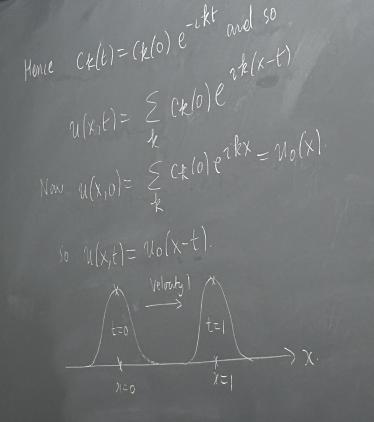
\includegraphics[width=0.5\linewidth]{Figures/lecture8/lec8-1.png}\]
    Alternatively, \textbf{suppose we use Euler to solve $(\star)$}, we then have that Euler scheme
    \[c_k^{n+1} = c_k^n - i kh c_k^n\]
    where $c^n_k \simeq c_k(nh)$. Hence, we have that
    \[c_k^n = (1 - i kh)^n c_k^0 = (1 - ikh)^n c_k(0)\]
    This method converges as $h \to 0$ and $n \to \infty$. \textbf{BUT!!!!!!} we observe that
    \[|c_k^n|^2 = (1 + k^2 h^2)^n |c_k^0|^2 = (1 + k^2 h^2)^n |c_k(0)|^2\]
    Compare with $|c_k(t)|^2 = |c_k(0)|^2$, but since $1 + k^2 h^2 > 1$ when $h \neq 0$, this solution will definitely explode for any $h \neq 0$! There is no sufficiently small $h$ that could make the Euler scheme better, it will blow up the calculation no matter what time step we pick. Similarly, when $k \neq 0$ (outside the constant frequency), any solution will also blow up.\\

    In this case, this shows that the Euler scheme is \textbf{unconditionally unstable} for this equation, that is
    \[\forall k \neq 0: |c_k^n| \to \infty \text{ as } n \to \infty\]
\end{example}

This leads us to the next question - \textbf{when is the Euler scheme stable?} The above example shows that - to study stability, it suffices to consider equations of the form
\[\frac{du}{dt} = \lambda u, \lambda \in \Cbb, \operatorname{Re}(\lambda) \leq 0.\]
The condition that $\operatorname{Re}(\lambda) \leq 0$ indicates that the problem is stable. Some examples are
\[\lambda = \begin{cases}
    - \epsilon k^2, \text{ if we are solving Fisher/Heat}\\
    -ik, \text{ One way wave}
\end{cases}\]

\begin{remark}
    By ``stability", we mean if our solution originally does not blow up, then our scheme shouldn't blow up either.
\end{remark}

With the Euler's method, we found that
\[\frac{u_{n+1}}{u_n} = R(h \lambda) = 1 + h\lambda\]
where $R(z)$ is called the \textbf{Stability function} and the region
\[\{z \in \Cbb: |R(z)| < 1\}\]
is called the stability region.

\begin{example}
    The Euler scheme is stable for $|1 + z| < 1$. In other words they are the points
    \[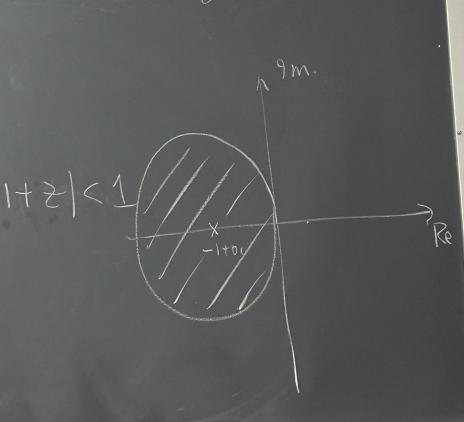
\includegraphics[width=0.5\linewidth]{Figures/lecture8/lec8-2.png}\]
    We then see that if our Fourier coefficients are inside the circle, it is okay and stable. The problem really occurs when the Fourier coefficients exit the circle.
\end{example}

\textbf{The HOLY GRAIL} for us is to try to extend the region of stability to the left half plane $\{z \in \Cbb\ |\ \operatorname{Re}(z) < 0\}$.

\begin{question}
    What goes wrong with Euler?
\end{question}

Suppose we start with $f(t, \lambda) = \lambda$ and $\lambda << -1$, then consider the plot
 \[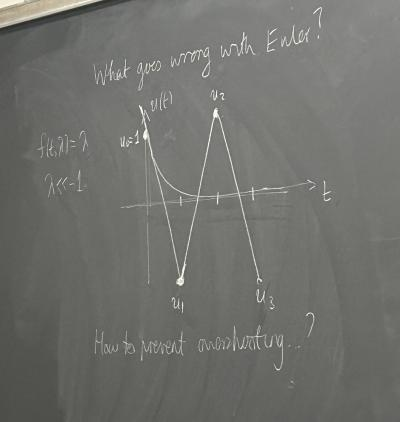
\includegraphics[width=0.5\linewidth]{Figures/lecture8/lec8-3.png}\]
At $t = 0$, the slope is very steep. If $h$ the time step is small, then it's fine. But if we have a big enough time step, it will have a large deviation at $t_1$. Then we want to go up again by a large margin. The problem is that the big time steps never lets Euler's method recover from this. Hence, this only works when $\lambda h$ is small (that is, it is in the region of convergence).\\

We need to ``lift out eyes and see where we're going". Recall that Euler was based on the left hand endpoint rule that does not look ahead:
\[\int_0^h g(t) dt \approx h g(0)\]
whereas the Trapezoidal rule looks ahead:
\[\int_0^h g(t) dt \simeq \frac{h}{2} [ g(0) + g(h) ]\]
Our scheme now becomes
\[u(t_{n+1}) = u(t_n) + \int_{t_n}^{t_{n+1}} f(s, u(s)) ds \]
\[u_{n+1} = u_n + \frac{h}{2} [f(t_n, u_n) + f(t_{n+1}, u_{n+1})]\]

Let's try to do a basic test for stability. We choose $f(t, u) = \lambda u$, then we have that
\[u_{n+1} = u_n + \frac{h}{2} [\lambda u_n + \lambda u_{n+1}]\]
Recall we defined the stability function as
\[R(h\lambda) \coloneqq \frac{u_{n+1}}{u_n}\]
Hence we have that
\[\frac{u_{n+1}}{u_n} = \frac{1 + \frac{h\lambda}{2}}{1 - \frac{h\lambda}{2}} = R(h\lambda)\]
Hence our stability function is
\[R(z) = \frac{1 + z/2}{1 - z/2}\]
Now we seek $z \in \Cbb$ such that $|R(z)| < 1$, which is satisfied if and only if $|1 + \frac{z}{2}| < |1 - \frac{z}{2}|$. This is the set of points that are closed to $-1$ than to $1$. In fact, this gives the entire left half plane!
 \[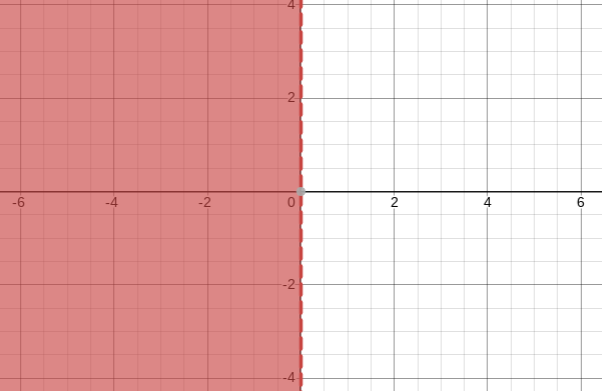
\includegraphics[width=0.5\linewidth]{Figures/lecture8/lec8-4.png}\]

\subsection{Crank-Nicolson Method}
This scheme is called the \textbf{Crank-Nicolson Method}. Here are some remarks:
\begin{enumerate}
    \item This will be stable for One-Way Wave Equation. In fact $R(ikh) = 1$ so we have that $|c_k(t)|$ is a constant!
    \item This will be stable for the Heat equation
    \[\frac{\partial u}{\partial t} = \epsilon \Delta u, \text{ Eigenvalues are $-\epsilon k^2$}\]
\end{enumerate}

\begin{question}
    What about the rate of convergence?
\end{question}

Let $e_n = |u(t_n) - u_n|$ be the error, then we have that
\begin{align*}
    e_{n+1} &= u(t_{n+1}) - u_{n+1}\\
    &= (u(t_n) - u_n) + \int_{t_n}^{t_{n+1}} u'(s) ds - \frac{h}{2} [f(t_n, u_n) + f(t_{n+1}, u_{n+1})]\\
    &=  (u(t_n) - u_n) + [\int_{t_n}^{t_{n+1}} u'(s) ds - \frac{h}{2} [u'(t_n) + u'(t_{n+1})]] + \frac{h}{2} [f(t_n, u(t_n)) + f(t_{n+1}, u_{n+1})] - \frac{h}{2} [f(t_n, u_n) + f(t_{n+1}, u_{n+1})]\\
\end{align*}
Estimating the second term using the Trapezoidal rule, by Peano's Kernel Theorem know that
\begin{align*}
    |\int_{t_n}^{t_{n+1}} u'(s) ds - \frac{h}{2} [u'(t_n) + u'(t_{n+1})]| &\leq \frac{1}{12} h^3 M_3
\end{align*}
where $M_3 = \max_{a \leq t \leq b} |u^{(3)}(t)|$. We will use Lipschitz to estimate the remaining terms, where
\begin{align*}
    \frac{h}{2} |f(t_n, u(t_n)) - f(t_n, u_n)| &\leq \frac{hL}{2} |u(t_n) - u_n| \tag*{$L$ is the Lipschitz constant}
\end{align*}
and furthermore we have
\[\frac{h}{2} |f(t_{n+1}, u(t_{n+1})) - f(t_{n+1}, u_{n+1})| \leq \frac{hL}{2} |u(t_{n+1}) - u_{n+1}|\]
Hence, combinging the terms gives us
\[e_{n+1} \leq e_n + \frac{h^3}{12} M_3 + \frac{hL}{2} e_n + \frac{hL}{2} e_{n+1}\]
\begin{itemize}
    \item If $\frac{hL}{2} > 1$, then this tells me nothing.`
    \item However, if $\frac{hL}{2} < 1$, then we combine like terms and get that
    \[e_{n+1} \leq \frac{1 + \frac{hL}{2}}{1 - \frac{hL}{2}} e_n + \frac{h^3 M_3}{12 (1 -\frac{hL}{2})}, n = 0, 1, ...\]
    \[ = R(hL) e_n + \frac{h^3 M_3}{12(1 - \frac{hL}{2})}\]
\end{itemize}
Let $S = \frac{h^3 M_3}{12(1 - \frac{hL}{2})}$, which we think of as a source term.\\

Now we have that
\[e_{n+1} \leq R e_n + S\]
We observe that
\[e_1 \leq S \text{ and } e_0 = 0\]
\[e_2 \leq RS + S\]
\[e_3 \leq R^2 S + R S + S\]
By Ainsworth's Principle of Maximum Laziness, we have that by induction
\[e_n \leq \frac{h^3 M_3}{12 (1 - \frac{hL}{2})} \frac{R(hL)^n - 1}{R(hL) - 1}\]

We observe that
\begin{align*}
    R(hL)^n &= \left( \frac{1 + \frac{hL}{2}}{1 - \frac{hL}{2}} \right)^n\\
    &= (1 + \frac{hL}{1 - \frac{hL}{2}})^n\\
    &\leq \exp \{\frac{nhL}{1 - \frac{hL}{2}}\} \tag*{$(1 + r)^n \leq e^{nr}$}
\end{align*}

Now, we have arrived at a theorem.

\begin{theorem}
    Let $\{u_n\}_{n=0}^N$ be the output of Crank-Nicolson. If $u \in C^3[a, b]$ and $\frac{hL}{2} < 1$, then
    \[\max_{0 \leq n \leq N} |u(t_n) - u_n| \leq \frac{h^2 M_3}{12 L} [\exp (\frac{L (b-a)}{1 - \frac{hL}{2}}) - 1]\]
\end{theorem}

\begin{remark}
    This estimate is simialr to Euler but better ...
    \begin{itemize}
        \item We get second order convergence $O(h^2)$ if $u \in C^3[a, b]$.
        \item We get a larger region of convergence!
    \end{itemize}
    But what happens if $u \in C^2[a, b]?$ That is this week's homework and more.
\end{remark}

This function looks good, but how can solve for $u_{n+1}$? Moreover, how do we know that the following functional equation is even solvable?
\[u_{n+1} = u_n + \frac{h}{2} [f(t_n, u_n) + f(t_{n+1}, u_{n+1})]\]

We would like a lemma to tell us this is well-defined.

\begin{lemma}
   Let $f$ be Lipschitz with constant $L$. If $\frac{hL}{2} < 1$, then Crank-Nicolson is well-defined. 
\end{lemma}

\begin{proof}
    It suffices to show that for all $t \in [a, b]$ and $s \in \Rbb$, there exists some $r$ such that
    \[r = s + \frac{h}{2} f(t, r)\]
    We define a sequence
    \[r^{i+1} = s + \frac{h}{2} f(t, r^i)\]
    with $r^0$ given. We look at the difference between terms in the sequence, reminiscient to the proof of Picard's theorem,
    \begin{align*}
        r^{i+1} - r^i &= \frac{h}{2} [f(t, r^i) - f(t, r^{i-1})]\\
        &\leq \frac{hL}{2} |r^i - r^{i-1}| \tag*{Lipschitz continuity}
    \end{align*}
    The rest follows as in the proof of Picard because $\frac{hL}{2} < 1$.
\end{proof}

Furthernore, the proof of this lemma tells us a possible method to solve for $(\dagger)$ where
\[u_{n+1} = u_n + \frac{h}{2} [f(t_n, u_n) + f(t_{n+1}, u_{n+1})] \quad (\dagger)\]
The proof suggests a way to solve this as
\[\Tilde{u}^0 = \text{ initial guess } \]
\[\Tilde{u}^{i+1} = u_n + \frac{h}{2} [f(t_n, u_n) + f(t_{n+1}, \Tilde{u}^i)], i = 0, 1, ...\]
This is called the corrector. What should we choose for $\Tilde{u}^0$? We should choose
\[\Tilde{u}^0 = u_n + h f(t_n, u_n) \quad (\text{Euler Predictor})\]

We could either
\begin{itemize}
    \item (a) Correct to convergence (which we will do this for now).
    \item (b) Stop after one step. Option (b) gives another method with
\[\Tilde{u}_{n+1} = u_n + h f(t_n, u_n)\]
\[u_{n+1} = u_n + \frac{h}{2} [f(t_n, u_n) + f(t_{n+1}, \Tilde{u}_{n+1})],\quad n = 0, 1, ...\]
This is called \textbf{Heun's method}.
\end{itemize}

For (a), we sort of run into a predicament. We have an outer iteration that runs very effectively. We showed that the whole scheme works for the left half plane and can do some many amazing things, but to find $\Tilde{u}^{i+1}$ as an approximate iteration, the inner iteration only converges when $\frac{hL}{2} < 1$, which is the same constraint as Euler's method!\\

We can resolve this by switching the inner iteration with another method. Fortunately, since we are workign with a speicfic $f$, we coudl fine tune into a more specific method. Consider
\[\frac{\partial u}{\partial t} = \epsilon \frac{\partial^2 u}{\partial x^2} + \lambda u + g(t, u) \quad (\star)\]
where $g$ is LIpschitz and $\epsilon  0$, $\lambda \geq 0$. When $g(t, u) = - \lambda u^2$, we get back Fisher's equation.\\

We seek a $2\pi$-periodic solution again of the form
\[u(x, t) = \sum_{k \in \Zbb} c_k(t) e^{ikx}\]
We insert this into $(\star)$ and equate the Fourier coefficients to find
\[\frac{d c_k}{dt} = (- \epsilon k^2 + \lambda) c_k + g_k(t, \Vec{c}), k \in \Zbb\]
where $g_k(t, \Vec{c}) = \frac{1}{2\pi} \int_{-\pi}^{+\pi} g(t, u) e^{-ikx} dx$. We discretize in time using Crank-Nicolson, we have that
\begin{align*}
    c_k^{n+1} &= c_k^n + \frac{h}{2} [(-\epsilon k^2 + \lambda) c_k^n + g_k(t_n, \Vec{c}^n) + (-\epsilon k^2 + \lambda) c_k^{n+1} + g_k(t_{n+1}, \Vec{c}^{n+1})] \quad (\spadesuit)
\end{align*}
The lemma tells us that we get convergence if $h$ is sufficiently small. How small? Well the Lipschitz constant for the mapping gives
\[r \mapsto (-\epsilon k^2 + \lambda) r + g_k(t, \Vec{r})\]
Note that the LINEAR TERM here is responsivle for a big Lipschitz constant for it to be $O(k^2 \epsilon)$. The non-linear term does not contribute much. If we don't have the lienar term but keep $g_k$, we should be in buisness!\\

Let's try a difficult rearrangement of the equation $(\spadesuit)$, let's combing like terms and find
\begin{align*}
    \{ 1 + \frac{k}{2} (\epsilon k^2 - \lambda)\} c_k^{n+1} &= c_k^n + \frac{h}{2} [(-\epsilon k^2 + \lambda) c_k^n + g_k(t_n, \Vec{C}^n) - g_k(t_{n+1}, \Vec{C}^{n+1}) ]\quad (\clubsuit)
\end{align*}
Now let's look at the scheme based on $(\clubsuit)$, which depends on the mapping
\[r \mapsto \frac{-\frac{h}{2} g_k(t_{n+1}, \Vec{r})}{1 + \frac{h}{2} (\epsilon k^2 - \lambda)}\]
which has the Lipschitz constant
\[\frac{\frac{h}{2} L_g}{1 + \frac{h}{2} (\epsilon k^2 - \lambda)}\]
This splits into 2 cases:
\begin{enumerate}
    \item If $\epsilon k^2 << 1$, then the term becomes
    \[\frac{\frac{h}{2} L_g}{1 - \lambda h/ 2} < 1\]
    \item If $\epsilon k^2 >> 1$, the term becomes
    \[\frac{L_g}{\epsilon k^2} \lesssim 1\]
\end{enumerate}

We conclude that - the nonlinear inner iterations converges for $h$ sufficiently small and is independent of $\epsilon$ and $k^2$. Moreover, we should get no waves as $k \to \infty$. This should work without having to change time steps!\\

This is called the \textbf{IMEX} method. The instructor then begins to give a demo of this.

\newpage
\section{Lecture 9}

\subsection{Debugging and Choosing Numerical Schemes}

Last week, even though we said the program theoretically shouldn't break with any number of nodes, it broke with $100$ nodes. Why is that?\\

Let's investigate. We consider the equation
\[\frac{du}{dt} = \lambda u (1 - u) = f(u).\]
From a dynamical systems perspective, the equilibriums looks like
\[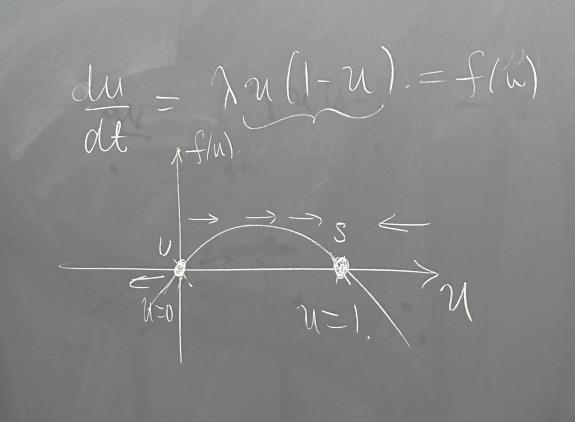
\includegraphics[width=0.6\textwidth]{Figures/lecture9/lec9-1.png}\]
This means we have an unstable equilibrium. If $u$ starts off very negative and far away from the stable equilibrium, this would diverge!\\

When we consider Fisher's equation, we have that
\[\frac{\partial u}{\partial t} = \epsilon \frac{\partial^2 u}{\partial t^2} + \lambda u(1 -u )\]
The nonlinear term does not break the program, but the problem was that the initial condition was too big! WHen we picked $100$ Fourier nodes, we have that $u(x, t) = \sum_{|k| \leq 100} c_k(t) e^{ikx}$ and $||u(\bullet, )||^2 = \sum_{|k| \leq 100} |c_k|^2$ will be large and indicate that the initial condition will slide off away from the stable solution.\\

Hence, we should try to rescale our coefficients
\[c_k \sim \frac{U[0, 1]}{\sqrt{1 + k^2}}, |c_k|^2 \sim \frac{1}{1+k^2}\]
which should be more stable.\\

For last week's homework, there's a lot of \textbf{controversy} over whether Fourier and Finite Difference is better than one another. Here's some misinformation.
\begin{enumerate}
    \item ``Fourier is only good for periodic" - this is actually not the case. While in class we only considered $u(0, t) = u(\pi, t)$. This could work for any boundary conditions.\\
    
    For example, if we suppose instead want to solve equations with boundary condition $u(0, t) = u(2\pi, t) = 0$. In this case, we can consider $u(x, t) =\sum_k c_k e^{ikx} = a_0 + \sum a_k \cos k x + b_k \sin kx$. If we set $a_0 = 0$ and $a_k = 0$, we get $u(x, t) = \sum_k b_k \sin k x$ which could work to be extended to $0$ to $2\pi$.\\

    For another example, if we consider $\frac{\partial u}{\partial x}(0, t) = \frac{\partial u}{\partial x}(2\pi, t) = 0$, then in this case we seek equations are the form $u(x, t) = a_0 + \sum a_k \cos k x$.

    \item ``Finite differences are only good for Dirichlet conditions" - you can still do periodic with Difference methods as well. You just start by renaming the coefficients when they start to repeat:
\[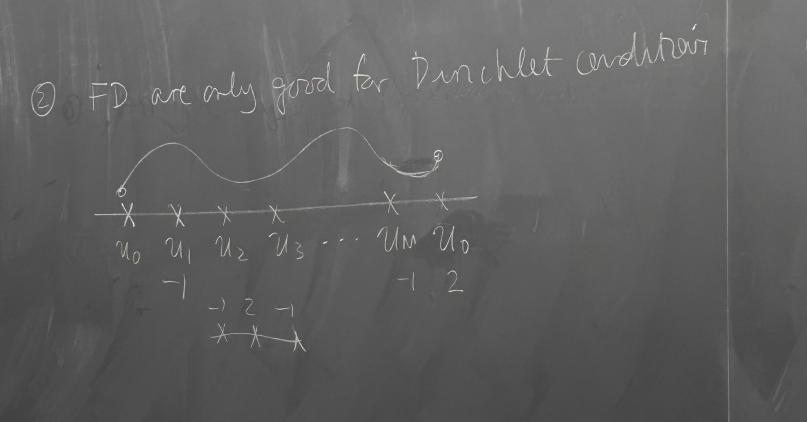
\includegraphics[width=0.6\textwidth]{Figures/lecture9/lec9-2.png}\]
\end{enumerate}

So what are the actual valid differences?
\begin{enumerate}
    \item The Fourier method does converge a lot faster than Finite Differences. We sketch the idea here.\\
    
    If we consider $u(x) = \sum_{k \in \Zbb} c_k e^{ikx}$ and $u_K(x) = \sum_{|k| \leq K} c_k e^{ikx}$, then we see that
    \[u(x) - u_k(x) = \sum_{|k|>K} c_k e^{ikx}\]
    On the other hand, we have that
    \[u_{xx} \simeq \frac{u(-r) - 2 u(0) + u(r)}{r^2} + O(r^2) u_{xxxx}\]
    Hence in terms of the Fourier coefficients, we know that
    \[u^{(4)}(x) = \sum_k (ik)^4 c_k e^{ikx} \]
    \[||u^{(4)}||^2 = \sum_k |k|^8 |c_k|^2 < \infty \implies c_k \sim k^{-4}\]
    Thus, the Fourier method converges at a rate of $k^{-4}$ as opposed to finite difference, which is around $k^{-2}$.
    \item Fourier series play nicely with differentiable operators. If we for example consider
    \[-\epsilon \frac{\partial^2 u}{\partial x^2} + b \frac{\partial u}{\partial x} + c u\]
    Then the homework allowed us to discrete this into a tridiagonal matrix $A$. But each time you want to move on in a time step, it couples nodes together. You would have to invert the tirdiagonal matrix and takes extra annoying working.\\

    On the other hand, if we do the Fourier method, the nodes aren't coupled together, and there's no matrices to invert here.
    \item On the other hand, there's a lot of convolutions to compute in the Fourier method which complicates the method. The discretization of derivatives into linear equations is a lot easier to compute. Nevertheless, the convolution is closer to the physics and gives a better idea on how the non-linearity works. For the example of Fisher's equation, we have that
    \[\frac{\partial u}{\partial t} = \epsilon \frac{\partial^2 u}{\partial x^2} + \lambda u - \lambda u^2 \]
    the terms $\epsilon \frac{\partial^2 u}{\partial x^2} + \lambda u$ are not mixing different frequencies. If we look at what's happening with the last term, we are looking at
    \[u \mapsto \frac{1}{2\pi} \int_{-\pi}^{\pi} u(x, t)^2 e^{-ikx} dx, k \in \Zbb\]
    \[\int (\sum_m c_m(t) e^{imx} ) (\sum_\ell c_\ell(t) e^{i\ell x}) dx = \sum_{\ell + m} c_m c_\ell \int e^{i(m + \ell - k)x}\]
    which is the direct delta function on $m + \ell = k$, hence the sum is
    \[= \sum c_m c_{k - m}.\]
    Hence Fourier conveys you an insight into the mixing of frequencies.
    \item The downside of Fourier is that it only works in tensor product domains, in the sese that it's of the form $[a_1, b_1] \times [a_2, b_2] \times ... \times [a_d, b_d]$. But if we have a domain like a Pac-Man, the Fourier method has no hope on it. Neither would finite difference work (where are you even gonna put the nodes properly). In this case, we need something like a finite element method, more to see in 2560.
    \item The Fourier transform diagnalizes differentiation.
\end{enumerate}

\begin{remark}
Historically, finite difference methods came first. Even the Euler method is an example of finite difference methods. Up to about the 1940s or 1950s, the finite difference methods have been the standard. The U.S. government also implemented a lot of code and machines strictly with the framework of finite differences methods.\\

In about 1970s, finite element methods came along. Embarrassingly, the engineers were the first to realize that they are good. Nowadays, finite element methods became the mainstream and pretty much everyone uses them.
\end{remark}

\subsection{Heun's Method - Two Step Runge Kutta Methods}

For the Crank-Nicolson method, we were considering the scheme
\[u_{n+1} = u_n + \frac{1}{2} h \{f(t_n, u_n) + f(t_{n+1}, u_{n+1})\}\]
is based on the Trapezoidal Rule. This is attractive because:
\begin{itemize}
    \item The stability region is the left-half plane (which we call it to be ``\textbf{A-stable}", meaning absolute stability).
    \item It is second order accurate.
\end{itemize}
It is unattractive possibly because 
\begin{itemize}
    \item It is implicit, because we need to solve $u_{n+1}$ in a non-linear system of equation, which is generally difficult. The RHS dpeends on the LHS.
\end{itemize}

\begin{question}
    Is there a related EXPLICIT scheme that retains the advantages of being A-stable and second order accurate?
\end{question}

Last time, we discovered \textbf{Heun's method} based on an explicit forward Euler predictor, where we say
\[u_{n+1} \simeq \Tilde{u}_{n+1} = u_n + h f(t_n, u_n)\]
We can get $\Tilde{u}_{n+1}$ explicitly, for which we then define
\[u_{n+1} \coloneqq u_n + \frac{h}{2} [f(t_n, u_n) + f(t_{n+1}, \Tilde{u}_{n+1})].\]

We have made the method explicit now, but the danger here is that we might lose a second order accuracy and no longer A-stable. Let's try to write this as an Algorithm:
\begin{tcolorbox}[standard jigsaw,opacityback=0]
\begin{algorithm}[H]
\caption{Heun's Method (Explicit Runge-Kutta 2)}
\KwData{$u_0 = u(a);$ and $f$}
\KwResult{The tuples approximating $(t_k; u(t_k))_{k = 0}^n$}
1. for $n = 0, 1, ..., N-1$, we compute $\{$\;
1a. $k_1 = f(t_n, u_n)$\;
1b. $k_2 = f(t_n +h, u_n + h k_1)$\;
1c. $u_{n+1} = u_n + \frac{h}{2} [k_1 + k_2]$$\}$\;
2. \text{// where $t_n = a + nh, h = \frac{b-a}{N}$}
\end{algorithm}
\end{tcolorbox}

\begin{question}
    What are its mathematical properties?
\end{question}

Let's start by looking at its stability. We consider the equation
\[\frac{du}{dt} = \lambda u, \lambda \in \Cbb, \text{ so } f(t, u) = \lambda u.\]
The scheme proceeds as follows:
\begin{itemize}
    \item We see that $h k_1 = h f(t_n, u_n) = h \lambda u_n$.
    \item It then follows that $h k_2 = h \lambda(u_n + h k_1) = h \lambda (1 + h \lambda ) u_n$.
\end{itemize}
We then see that
\begin{align*}
    \frac{u_{n+1}}{u_n} &= 1 + \frac{1/2(h k_1 + h k_2)}{u_n}\\
    &= R(h\lambda)
\end{align*}
where $R(z) = 1 + z + \frac{1}{2} z^2$.

\begin{remark}
We recall what the stability functions for other approximation methods are:
\begin{enumerate}
    \item Euler-Scheme: $R(z) = 1 + z$.
    \item Crank-Nicolson: $R(z) = \frac{1 + z/2}{1 - z/2}$.
    \item Heun's Method: $R(z) = 1 + z + \frac{z^2}{2}$
\end{enumerate}
which are all roughly exponential approximating $e^z$. This phenonmenon is called \textbf{Padé Approximation}. 
\end{remark}

The stability region for Heun's method is $\{z \in \Cbb: |R(z)| < 1\}$. This is clearly not A-stable because as $|z| \to \infty$, $|R(z)|$ will go to infinity. Let $z$ belong to the stability region for Euler, ie. $|1 + z| \leq 1$, then 
\begin{align*}
    |R(z)| &= |1 + z + \frac{1}{2} z^2|\\
    &= |\frac{1}{2} (z + 1)^2 + \frac{1}{2}|\\
    &\leq \frac{1}{2} |1 + z|^2 + \frac{1}{2}\\
    &\leq 1
\end{align*}
This shows that Heun's method has a stability regio that contains Euler's stability region!\\

This is approximately what the stability region of Heun's method (outer) compare to Euler's method (inner):
\[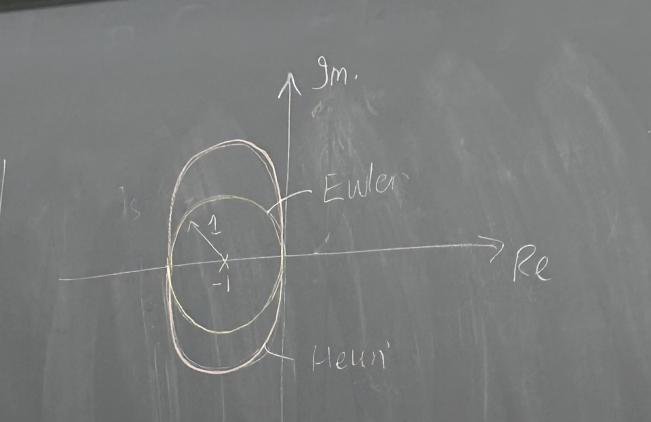
\includegraphics[width=0.6\textwidth]{Figures/lecture9/lec9-3.png}\]

\begin{question}
Now, does Heun's method retain the second order accuracy of Crank-Nicolson?
\end{question}

Let's write Heun's method as follows:
\begin{itemize}
    \item Let $v_1 = u_n$ and $v_2 = u_n + h f(t_n, u_n)$
    \item $v_1$ is an approximation of $u(t_n)$ and $v_2$ is an approximation of $u(t_{n+1})$.
    \item Heun's step tells us to do
    \[u_{n+1} = u_n + \frac{h}{2} \{f(t_n, v_1) + f(t_{n+1}, v_2)\}\]
\end{itemize}
Now, let $e_n = |u(t_n) - u_n|$, then we have that
\begin{align*}
    u(t_{n+1}) - u_{n+1} &= u(t_{n}) + \int_{t_n}^{t_{n+1}} f(s, u(s)) ds - u_n -  \frac{h}{2} \{f(t_n, v_1) + f(t_{n+1}, v_2)\}\\
    &= [u(t_n) - u_n] + [\int_{t_n}^{t_{n+1}} u'(s) ds - \frac{h}{2} \{u'(t_n) + u'(t_{n+1})\}] + \frac{h}{2} \{f(t_n, u(t_n)) - f(t_n, v_1)\}\\&+ \frac{h}{2} \{f(t_{n+1}, u(t_{n+1})) - f(t_n, v_2)\} \tag*{Add Zero}
\end{align*}
The second term is the error in using Trapezoidal rule bounded by $\frac{1}{12} h^3 M_3$. The remaining terms estimated using the Lipschitz property gives
\[\frac{1}{2} h L |u(t_n) - v_1| \text{ and } \frac{1}{2} hL |u(t_{n+1}) - v_2|\]
First one is just $\frac{1}{2} h L e_n$. The second one is new to us and we have
\begin{align*}
    u(t_{n+1}) - v_2 &= u(t_{n+1}) - (u_n + h f(t_n, u_n))
\end{align*}
This reminds us of the error term for the Euler-scheme, so let's argue as we did for Euler. What we then get is that
\begin{align*}
    u(t_{n+1}) - v_2 &= u(t_n) - u_n + \int_{t_n}^{t_{n+1}} u'(s) ds - h u'(t_n) + h \{f(t_n, u(t_n) - f(t_n, u_n)\}
\end{align*}
Estimating this using the Left Hand End Point Ruler, we have that
\[|u(t_{n+1}) - v_2| \leq e_n + \frac{1}{2} h^2 M_2 + hL e_n\]

Combining everything together, we obtain that
\[e_{n+1} \leq e_n \{1 + \frac{1}{2} hL + \frac{1}{2} hL + \frac{1}{2} (hL)^2\} + \frac{1}{12} h^3 M_3 + \frac{1}{2} hL (\frac{1}{2} h^2 M_2)\]
\[= R(hL) e_n + \frac{1}{12} h^3 \{M_3 + 3 L M_2\}\]

Solving as usual gives
\[e_n \leq \frac{R(hL)^n - 1}{R(hL) - 1} \frac{h^3}{12} (M_3 + 3 L M_2),  n = 0, 1, ...\]

Now, we have that
\begin{align*}
    R(hL) &= 1 + hL + \frac{1}{2} (hL)^2\\
    &\leq e^{hL}
\end{align*}
and $R(hL) - 1 = hL (1 + \frac{1}{2} hL)$. Finally, we obtain a theorem:

\begin{theorem}
    Let $\{u_n\}_{n = 0}^N$ be the outputs of Heun's method with $h = \frac{b - a}{N}$, then we have that
    \[\max_{0 \leq n \leq N} |u(t_n) - u_n| \leq \frac{h^2}{12L} \frac{M_3 + 3 L M_2}{1 + \frac{1}{2} hL} \{e^{L(b-a)} - 1\}\]
\end{theorem}

In conclusion, even though Euler forms part of Heun's method, it doesn't pollute or reduce the order of accuracy. However, it has a much smaller region of stability compared to Crank-Nicolson. 

\subsection{Alternative Derivation of Heun's Method}
The plot twist is that the above proof is not usually how textbooks do it. This is how textbooks usually do it. Consider the scheme having the general form
\[u_{n+1} = u_n + h \{b_1 f(t_n, u_n) + b_2 f(t_{n} + ch, u_n + a h f(t_n, u_n))\}\]
where $b_1, b_2, c, a$ are all to be determined. Heun's method corresponds to $c = 1, a = 1, b_1 = b_2 = \frac{1}{2}$, but can we do better with different choices?\\

Assuming that everything is smooth, we can try a wild Taylor expansion and see that
\begin{align*}
    f(t_n + ch, u_n + ah f(t_n, u_n)) &= f(t_n, u_n) + h \{c \frac{\partial f}{\partial t}(t_n, u_n) + a f(t_n, u_n) \frac{\partial f}{\partial u}(t_n, u_n)\} + h^2 \{a \frac{\partial^2 f}{\partial t \partial u} (t_n, u_n) + ...\} + O(h^3)
\end{align*}
So the scheme satisfies
\[u_{n+1} = u_n + h (b_1 + b_2) f(t_n, u_n) + h^2 b_2 \{c \frac{\partial f}{\partial t}(t_n, u_n) + a f(t_n, u_n) \frac{\partial f}{\partial u}(t_n, u_n) \} + O(h^3)\]
Now we compare this with the Taylor series of the true solutions, that is
\[u(t_{n+1}) = u(t_n) + h u'(t_n) + \frac{1}{2} h^2 u''(t_n) + O(h^3)\]
\[ = u(t_n) + h f(t_n, u(t_n)) + \frac{1}{2} h^2 [\frac{d}{dt} f(t, u(t))]|_{t=t_0} + O(h^3)\]
where $\frac{d}{dt} f(t, u(t)) = \frac{\partial f}{\partial t}(t, u(t)) + u'(t) \frac{\partial f}{\partial u}(t, u(t)) =  \frac{\partial f}{\partial t}(t, u(t)) + f(t, u(t)) \frac{\partial f}{\partial u}(t, u(t))$.\\

Comparing the coefficients of terms between the true solution and the scheme, we see that
\begin{itemize}
    \item $b_1 + b_2 = 1$
    \item $c b_2 = \frac{1}{2}$
    \item $a b_2 = \frac{1}{2}$
\end{itemize}
Solving the $3$ non-linear equations, now the scheme is therefore 
\[u_{n+1} = u_n + h \{(1 - \theta) f(t_n, u_n) + \theta f(t_n + \frac{h}{2 \theta}, u_n + \frac{h}{2 \theta} f(u_n, t_n)\} \]
Heun chooses $\theta = \frac{1}{2}$. Clearly this decays at rate of $h^2$ because of how the Taylor series compare.

\begin{remark}
    The same argument can be used for any order, but gets quite messy. For example, for order $9$, we end up with $486$ non-linear equations.
\end{remark}

There still remains a question - is our new $\theta$-scheme better than Heun? We already know they have the same order of accuracy, but may be there's a bigger stability region?\\

Let's try to do a stability analysis. Let $f(t, u) = \lambda u$ with $\lambda \in \Cbb$, so we have that
\[\frac{u_{n+1}}{u_n} = 1 + (1 - \theta) h \lambda + \theta h \lambda (1 + \frac{h \lambda}{2 \theta}) = 1 + h \lambda + \frac{1}{2} (h \lambda)^2\]
which is independent of $\theta$!\\

The instructor then proceeded to give a demo of Heun's method.\\

The demo suggested that rather than a uniform grading using Heun's method, maybe we should try to look for an adaptive method. Why don't we try to compare the error estimator between the difference of the two terms
\[v_2 = u_n + h f(t_n,u_n) = u(t_{n+1}) + O(h^2)\]
\[u_{n+1} = u_n + .... = u(t_{n+1}) + O(h^3)\]
We will think more about this next lecture.

\end{document}